\chapter{函数空间}
\label{chap:functional-analysis-and-approximation}

\newcommand{\functionalinlinetablecaption}[2]{%
  \refstepcounter{table}\label{#1}%
  \addcontentsline{lot}{table}{\protect\numberline{\thetable}#2}%
  \par\smallskip\noindent
  {\figurefont\footnotesize
   \textcolor{BookTeal}{表~\thetable}\quad #2}\par}
\newcommand{\functionalinlinefigurecaption}[2]{%
  \refstepcounter{figure}\label{#1}%
  \addcontentsline{lof}{figure}{\protect\numberline{\thefigure}#2}%
  \par\smallskip\noindent
  {\figurefont\footnotesize
   \textcolor{BookTeal}{图~\thefigure}\quad #2}\par}

拟合一条曲线时，有限维模型常把函数写成固定基函数的线性组合：
\begin{equation}
  f_m(x)=\sum_{j=1}^{m}a_j\phi_j(x).
  \label{eq:functional-finite-basis-expansion}
\end{equation}
当$m$固定时，可以把系数$(a_1,\ldots,a_m)^{\top}$当作普通向量，用欧氏距离比较两个
候选解。然而，一旦允许基函数数目增加，系数向量所在的维数也随之改变；同一个函数还可能
在不同基下拥有完全不同的系数。此时，仅比较参数向量已经不能稳定地回答函数
之间相差多少、有限表示能否逼近目标，以及有限观测究竟确定了哪些函数方向。


上一章的点可以作为函数的输入位置，上一章的度量与体积可以规定函数的局部变化与整体误差。
本章则把整个函数作为一个可变对象：$f(x)=a+bx$由两个系数确定，
$x$是读取位置，$(a,b)$是函数的记录。以下主要研究实函数与实Hilbert空间；
复内积仍遵循第一变量共轭线性的约定，此时线性读取应写为$\ell_h(f)=\langle h,f\rangle$。

本章先说明函数可以怎样表示与比较，再建立投影、读取、积分和微分运算。
这些运算分别用于最近函数、有限观测拟合、整体误差拟合与平滑能量求解。
求得候选以后，还要检验展开、表示规模和采样变化所产生的逼近，以及扰动后的响应。
其中始终保留两个变量的区别：对输入位置求导描述函数的空间变化，
对未知函数作扰动则描述目标如何评价候选变化。
\section{元素与表示}
\label{sec:functional-functions-as-space-elements}

仿射函数可以用两个系数记录，也可以用两个点值记录；有限读数是否足够，取决于候选范围。
本节先界定函数对象，再说明系数、展开与读数怎样产生。
从这些信息反求未知函数的条件，则留到拟合问题中建立。

\subsection{函数与空间的界定}
\label{sec:functional-objects}

设$\mathcal{X}$为输入集合，$\mathbb{R}^{\mathcal{X}}$表示从$\mathcal{X}$到
$\mathbb{R}$的全部函数。对$f,g\in\mathbb{R}^{\mathcal{X}}$和$a,b\in\mathbb{R}$，
定义
\[
  (af+bg)(x)=af(x)+bg(x),\qquad x\in\mathcal{X}.
\]
这些逐点运算使$\mathbb{R}^{\mathcal{X}}$成为向量空间。式
\eqref{eq:functional-finite-basis-expansion}描述的集合只是其中由
$\phi_1,\ldots,\phi_m$张成的有限维子空间。允许无限多个基方向以后，线性结构仍然
存在，但坐标数目不再适合作为唯一的大小尺度。



向量值函数$f:\mathcal X\to\mathbb R^r$也可逐点线性组合。
流形上的向量场则在每个$p$取值于$T_p\mathcal M$，同点可相加，
跨点比较还须使用第\ref{sec:geometry-tangent-transport}节的搬运规则。
输入空间的维数并不决定函数空间的维数：区间只有一个输入坐标，
其上所有多项式却包含任意多个线性无关方向。

\subsection{函数的表示}
\label{sec:functional-representations}

固定线性无关的$(\phi_1,\ldots,\phi_m)$时，
式~\eqref{eq:functional-finite-basis-expansion}给出一个有限维子空间的坐标。
若方向相关，同一函数可以有多个系数记录。一般参数族$f_\theta$也不一定是线性子空间；
例如固定节点数的非线性神经网络族未必对加法封闭。

允许无限展开时，$\sum_j a_j\phi_j$先是一种待检验的记录形式：
它是否收敛、按什么距离收敛、结果是否仍是候选函数，都需要证明。
第\ref{sec:functional-decomposition-projection}节建立正交分量，
第\ref{sec:functional-truncation-convergence}节再研究其截断序列。

\subsection{函数表示的转换}
\label{sec:functional-representation-conversions}

有限基之间的转换沿用第\ref{sec:linear-algebra-coordinate-conversions}节。
以$f(t)=a+bt$为例，在基$(1,t-c)$中系数变为$(a+bc,b)$。
若记录已知函数的两个读数，选$t=0,1$便有
\[
 \begin{bmatrix}f(0)\\f(1)\end{bmatrix}
 =\begin{bmatrix}1&0\\1&1\end{bmatrix}\begin{bmatrix}a\\b\end{bmatrix}.
\]
这次转换可逆；只记录$f(0)$则丢失斜率方向。
一般已知系数到读数的矩阵元素为$L_i(\phi_j)$，
点值时是$\phi_j(x_i)$，积分时是$\int\phi_jw_i\,\mathrm d\mu$。
按这些规则计算记录不等于有限信息已经识别任意未知函数；
后者须限定候选范围并在拟合任务中判断。

\section{关系与结构}
\label{sec:functional-relations}

同样定义在一个区间上的多项式、连续函数与平方可积函数，允许的变化范围不同。
下面先比较这些候选集合的包含关系，再规定整体差异的大小。
积分误差还会忽略零测集上的变化，需要用等价关系明确空间中什么算同一个元素。

\subsection{函数集合的包含关系}
\label{sec:functional-inclusion-relations}

固定定义域后，$\operatorname{span}\{\phi_1,\ldots,\phi_m\}$包含于全函数空间，
若各$\phi_j$连续，还包含于连续函数集合。非线性参数族可以是其中的子集，
却未必是子空间。增加参数或方向可能扩大候选集合，但并未证明它能逼近所有目标。

测度还决定积分成员条件。设$0<\mu(\mathcal X)<\infty$，$1\leq p<q<\infty$，
Hölder不等式给出
\[
 \lVert f\rVert_{L^p}\leq
 \mu(\mathcal X)^{1/p-1/q}\lVert f\rVert_{L^q}.
\]
所以$L^q(\mu)\subseteq L^p(\mu)$；$q=\infty$时由本质上界直接得到同样结论。
无限测度下不能沿用这项包含：实轴上的常函数$1$有界却不属于有限$p$的$L^p$。

紧定义域上的连续函数有界，有限Borel测度保证其属于各有限$p$的积分范围。
进入$L^p$时采用自然映射$f\mapsto[f]_\mu$，输出是几乎处处等价类。
测度全支撑时，该映射单射：非零连续差在某个非空开集上绝对值有正下界，
而这个开集有正测度，故其等价类不为零。
若测度只集中于一个点，许多不同连续函数会给出同一个等价类。
集合成员、记录方式与映射是否丢失信息须分别说明。

\subsection{函数的距离关系}
\label{sec:functional-distance-relations}

如果要保证每个输入上的误差都小，就应控制全域最大偏差。
紧区间$[a,b]$上的连续函数空间$C([a,b])$为此常使用一致范数
\[
  \lVert f\rVert_{\infty}
  =\sup_{x\in[a,b]}|f(x)|.
\]
这个范数控制每个输入上的最大误差。若$\mu$是一个测度，则第
\ref{chap:mathematical-analysis}章建立的$L^p(\mu)$空间使用
\[
  \lVert f\rVert_{L^p(\mu)}
  =
  \left(\int_{\mathcal{X}}|f(x)|^p\,\mathrm{d}\mu(x)\right)^{1/p},
  \qquad 1\leq p<\infty.
\]
它控制的是相对于$\mu$的整体误差，允许函数在小测度集合上偏离较大。两种误差不能互相
替代。



这里先在可测代表上计算积分误差；正定性需要下一小节的归并。
加权误差相当于改变测度，权重退化时还会忽略原本可见的区域。
系数距离也取决于基：在$[-1,1]$及$\mathrm d\mu=\mathrm dt/2$下，
仿射函数差$\delta a+\delta bt$满足
\[
 \lVert\delta a+\delta bt\rVert_{L^2(\mu)}^2
 =(\delta a)^2+(\delta b)^2/3,
\]
而系数Euclidean距离平方为$(\delta a)^2+(\delta b)^2$。
固定有限基时可用Gram矩阵换算；维数增长或基变化时，不能默认误差常数统一。

\subsection{函数的等价关系}
\label{sec:functional-equivalence-relations}

积分半范数的零方向是几乎处处为零的可测函数。
沿用第\ref{sec:linear-algebra-equivalence-relations}节的商空间构造，
把$f=g$几乎处处的代表归为一个元素，才得到$L^p$中的真正范数。
若另用退化权重，零方向由该加权测度决定，而不是由原测度自动决定。

点值读取未必在这个商空间上良定义：改动单点可以不改变等价类却改变读数。
具有连续代表且测度全支撑时，连续代表唯一，才可据它读取点值；
另一些空间会直接把函数值作为对象的一部分。
有限观测产生的等价又不同。例如只读取仿射函数$f(0)$，
同截距函数的读数相同，但它们在整个区间上的积分距离可以非零。
观测等价只忽略观测不可见方向，不能替代整体函数相同。

\section{运算与映射}
\label{sec:functional-operators}

对整函数进行运算，可以取出某组方向上的分量、读出一个标量，或生成另一条函数。
下面依次建立投影、读取、积分变换与空间微分，最后说明目标对未知函数怎样求微分。
映射的叠加与复合仍沿用第~\ref{chap:linear-algebra-and-matrix-analysis}章的规则，但无限维中线性作用未必有界；
每一步还须检查定义域，保证前一步输出属于后一步可作用的函数范围。

\subsection{函数的分解与投影}
\label{sec:functional-decomposition-projection}
\label{sec:functional-orthogonal-expansions-projections}

\label{sec:functional-projection-approximation}

有限维正交化只处理有限基。无限维中，寻找最近分量往往先产生近似序列，
若空间缺少其极限，或候选不保留环境中的极限，就可能没有可用的投影。
因此在继续计算前，需要检查空间和子集各自保留什么极限。
若$\langle f,g\rangle=0$，称$f$与$g$正交。长度为$1$且两两正交的一组方向称为
正交归一方向；对非零$f,g$，比值
$\langle f,g\rangle/(\lVert f\rVert\lVert g\rVert)$落在$[-1,1]$内，可以解释夹角。
这里的方向是整函数，例如在$[-1,1]$的积分内积下，常函数$1$与函数$x$正交，
因为$\int_{-1}^1x\,\mathrm dx=0$，而不是因为它们的图像在平面中垂直。

$L^2(\mu)$是基本的内积空间，其内积为
\[
  \langle f,g\rangle_{L^2(\mu)}
  =\int_{\mathcal{X}}f(x)g(x)\,\mathrm{d}\mu(x).
\]
这个积分确实有限，因为$2|fg|\leq |f|^2+|g|^2$；正定性则使用了几乎处处等价类的约定。

后面的完备性证明会用到$L^2$版本的\term{Minkowski不等式}
（Minkowski inequality），也就是$L^2$范数的三角不等式。对$f,g\in L^2(\mu)$，
Cauchy--Schwarz不等式给出
\[
  \begin{aligned}
  \lVert f+g\rVert_{L^2(\mu)}^2
  &=
  \lVert f\rVert_{L^2(\mu)}^2
  +
  2\int_{\mathcal{X}}f(x)g(x)\,\mathrm{d}\mu(x)
  +\lVert g\rVert_{L^2(\mu)}^2\\
  &\leq
  \bigl(
    \lVert f\rVert_{L^2(\mu)}
    +
    \lVert g\rVert_{L^2(\mu)}
  \bigr)^2.
  \end{aligned}
\]
两边开平方便得到
$\lVert f+g\rVert_{L^2(\mu)}
\leq\lVert f\rVert_{L^2(\mu)}+\lVert g\rVert_{L^2(\mu)}$；
反复使用即可控制有限个函数之和。

例如不断截断一个无穷展开，每个候选只用有限个方向，而极限可能需要无穷多个方向。
如果只允许有限表示，序列即使内部越来越接近，也可能在候选空间之外达到极限。
分析章的完备性在这里要求：凡是按所选范数形成柯西序列的候选，
其极限都应仍由空间中的一个元素表示。
\begin{definition}[Banach空间]
\label{def:functional-banach-space}
若赋范空间$\mathcal V$在诱导距离$d(f,g)=\lVert f-g\rVert_{\mathcal V}$下完备，
即每个范数柯西序列都在该范数下收敛到$\mathcal V$中的元素，则称其为
\term{Banach空间}（Banach space）。
\end{definition}
完备性不负责证明某个具体
序列是柯西序列；它只保证一旦误差足以让序列内部彼此靠近，极限不会落到空间之外。

\begin{definition}[Hilbert空间]
\label{def:functional-hilbert-space}
在内积诱导的范数下完备的实内积空间称为\term{Hilbert空间}（Hilbert space）。
\end{definition}
因此，Hilbert空间也是Banach空间，但一般Banach空间不一定有与原范数相容的内积。
“赋范空间加完备性”与“内积空间加完备性”分别得到这两个名称，不是对同一种
结构的两种称呼。

区间$[a,b]$上的$C([a,b])$配备一致范数是Banach空间。事实上，若$(f_n)$在一致范数
下为柯西序列，那么每个$x$处的$(f_n(x))$都是实数柯西序列，可以定义
$f(x)=\lim_n f_n(x)$。柯西条件对所有$x$使用同一个$N$，故$f_n$一致收敛到$f$；
连续函数的一致极限仍连续，所以$f\in C([a,b])$。

同一个函数集合换一种范数可能失去完备性。连续函数空间$C([0,1])$配备$L^2$范数就
不是完备的。令$q(x)=\mathbb{I}\{x>1/2\}$，对$n\geq2$取
\[
 f_n(x)=
 \begin{cases}
  0,&x\leq1/2,\\
  n(x-1/2),&1/2<x<1/2+1/n,\\
  1,&x\geq1/2+1/n.
 \end{cases}
\]
每个$f_n$连续，且$\lVert f_n-q\rVert_2^2=1/(3n)$，
所以$(f_n)$在$L^2$中为柯西列。若连续函数$g$几乎处处等于$q$，
连续性迫使$g$在$(0,1/2)$恒为零、在$(1/2,1)$恒为一，因而无法在$1/2$处连续。
故这个极限没有任何处处连续的代表元。完成这个空间需要加入可测函数的几乎处处等价类，得到
$L^2([0,1])$。这里“几乎处处等价”很关键：如果$f$与$g$只在零测集上不同，它们在
$L^2$中是同一个元素。

$L^2(\mu)$本身的完备性可以从柯西列内部构造极限。设$(f_n)$在$L^2(\mu)$中为
柯西列。由柯西条件，选取递增的阈值$N_k$，使任意$m,n\geq N_k$时
$\lVert f_m-f_n\rVert_{L^2}\leq2^{-k}$。再递归选取严格递增的指标
$n_k\geq N_k$，就得到子列$(f_{n_k})$满足
\[
  \lVert f_{n_{k+1}}-f_{n_k}\rVert_{L^2(\mu)}
  \leq 2^{-k}.
\]
令$h_k=|f_{n_{k+1}}-f_{n_k}|$。对有限部分和反复使用上面的$L^2$版Minkowski
不等式，再用Fatou引理，可得
\[
  \int_{\mathcal{X}}
  \left(\sum_{k=1}^{\infty}h_k\right)^2
  \,\mathrm{d}\mu
  \leq
  \left(\sum_{k=1}^{\infty}2^{-k}\right)^2
  <\infty.
\]
因此$\sum_k h_k(x)$几乎处处有限，$(f_{n_k}(x))$在这些点绝对收敛。把它的几乎处处
极限记为$f$。同样对尾和使用Fatou引理，得到
\[
  \lVert f_{n_\ell}-f\rVert_{L^2(\mu)}
  \leq
  \sum_{k=\ell}^{\infty}2^{-k}
  \longrightarrow0.
\]
这个极限确实属于$L^2(\mu)$：令$H=\sum_k h_k$，前面的估计说明$H\in L^2$，
而$|f|\leq |f_{n_1}|+H$几乎处处成立，再用三角不等式即可。没有这一步，
仅仅构造出逐点极限还没有得到空间内的极限。
为把子列收敛传给原列，给定$\varepsilon>0$，先由柯西性取$N$，使$m,n\geq N$时
$\lVert f_m-f_n\rVert_{L^2}<\varepsilon/2$。再取$k$使$n_k\geq N$且
$\lVert f_{n_k}-f\rVert_{L^2}<\varepsilon/2$。于是每个$n\geq N$都满足
$\lVert f_n-f\rVert_{L^2}\leq\lVert f_n-f_{n_k}\rVert_{L^2}
+\lVert f_{n_k}-f\rVert_{L^2}<\varepsilon$，故整列也收敛到$f$。
这个论证同时说明为何要把只在零测集上不同的代表元视为同一元素：构造得到的点态极限
本来就只在几乎处处意义下确定。对$1\leq p<\infty$可用相同的可求和子列思路证明
$L^p(\mu)$完备；$p=\infty$时则控制本质上确界。因此，$1\leq p\leq\infty$时的
$L^p(\mu)$都是Banach空间，而前面已给出的内积使$L^2(\mu)$成为Hilbert空间。

有限表示可能并未包含极限，却能任意接近它；这项逼近性质应与空间的完备性分开。
\begin{definition}[稠密子集]
\label{def:functional-density}
设$(\mathcal V,\lVert\cdot\rVert)$为赋范空间，$\mathcal F\subseteq\mathcal V$。
若对每个$f\in\mathcal V$和每个$\varepsilon>0$，存在$g\in\mathcal F$满足
$\lVert f-g\rVert<\varepsilon$，则称$\mathcal F$在$\mathcal V$中稠密。
等价地，$\mathcal F$在该范数诱导距离下的闭包等于$\mathcal V$。
\end{definition}
这里的闭包由原集合及所有能被它任意接近的点组成；稠密不要求这些点已属于$\mathcal F$。
完备性与稠密性也不能混为一谈。
$\ell^2$由平方可和序列$\bm{a}=(a_1,a_2,\ldots)$组成，范数为
$\lVert\bm{a}\rVert_2^2=\sum_{j=1}^{\infty}a_j^2$。只有有限个非零坐标的序列构成
子空间$c_{00}$，它在$\ell^2$中稠密却不闭。序列
$(1,1/2,\ldots,1/n,0,\ldots)$属于$c_{00}$，其极限
$(1,1/2,1/3,\ldots)$属于$\ell^2$但不属于$c_{00}$。这正是闭性在最佳逼近问题中
不能省略的原因。有限截断能够不断逼近$\ell^2$中的元素，说明$c_{00}$的闭包是
$\ell^2$；它并不说明$c_{00}$自身已经包含这些极限。

把缺失的极限补进空间，称为空间完备化。其构造并不需要先猜出极限是什么函数：
取$\mathcal V$中的全部柯西列，规定
$(f_n)\sim(g_n)$当且仅当$\lVert f_n-g_n\rVert\to0$。
等价类$[(f_n)]$代表一个待补入的极限，逐项相加与数乘定义线性运算，范数定义为
\[
 \bigl\lVert[(f_n)]\bigr\rVert=\lim_n\lVert f_n\rVert.
\]
反三角不等式保证右边存在且与代表无关；范数为零恰好表示零等价类。
原空间通过常值列嵌入，新空间中的每个元素都能被原空间元素逼近。
这里稠密性也可直接验证：若$u=[(f_n)]$，则常值列所代表的$f_k$到$u$的距离为
$\lim_n\lVert f_k-f_n\rVert$，随$k\to\infty$趋于零。
新空间也完备：对其中的柯西列$(u_k)$，由稠密性选$v_k\in\mathcal V$使
$\lVert v_k-u_k\rVert<2^{-k}$，则$(v_k)$为$\mathcal V$中的柯西列，
其等价类记为$u$。按完备化中的距离定义，
\[
 \lVert u_k-u\rVert\leq2^{-k}+
 \lim_{\ell\to\infty}\lVert v_k-v_\ell\rVert.
\]
内层极限先固定$k$，计算$v_k$到$u$的距离；再令$k\to\infty$。
由于$(v_k)$为柯西列，充分大的$k,\ell$使两项之间的距离任意小，
所以右侧随$k\to\infty$趋于零。
若原空间有内积，则
\[
 \bigl\langle[(f_n)],[(g_n)]\bigr\rangle
 =\lim_n\langle f_n,g_n\rangle
\]
由Cauchy--Schwarz和柯西列有界性保证存在、与代表无关，并延伸原内积。
这样内积空间的完备化就是Hilbert空间。

闭性是相对于已指定的环境空间而言的；稠密性问原集合能否接近环境中的每个点；
完备化则把缺少的范数极限加入对象集合。它与分析章的测度完备化不同：
后者扩充可测集合并处理零测集的子集，不是在函数空间中补入柯西列的极限。
此外，一般Hilbert空间不必有可数稠密子集，不能预先假定它的全部方向都能列成一个序列。


闭子集保留环境中已有的极限；在完备空间中，闭子空间因此继承完备性。
只有Banach完备性还不够完成正交计算，下面还使用Hilbert内积的平行四边形恒等式。
\begin{theorem}[闭线性子空间的正交投影]
\label{thm:functional-closed-subspace-projection}
设$M$为实Hilbert空间$\mathcal H$的闭线性子空间。
每个$f\in\mathcal H$唯一写为$f=p+r$，其中$p\in M$、$r\in M^\perp$；
$p$是$M$中到$f$最近的元素，记为$P_Mf$。
\end{theorem}
\begin{proof}
令$d=\inf_{u\in M}\lVert f-u\rVert$，取$u_n\in M$使$\lVert f-u_n\rVert\to d$。
因为$(u_n+u_k)/2\in M$，平行四边形恒等式给出
\[
\begin{aligned}
 \lVert u_n-u_k\rVert^2
 &=2\lVert f-u_n\rVert^2+2\lVert f-u_k\rVert^2\\
 &\quad-4\left\lVert f-\tfrac12(u_n+u_k)\right\rVert^2\\
 &\leq2\lVert f-u_n\rVert^2+2\lVert f-u_k\rVert^2-4d^2\to0.
\end{aligned}
\]
完备性给出极限$p$，闭性使$p\in M$，范数连续性使$\lVert f-p\rVert=d$。
对任意$h\in M$，$p+th$仍可行，展开其距离平方，
在$t=0$取得极小便有$\langle f-p,h\rangle=0$。
若$p_1+r_1=p_2+r_2$为两种分解，差属于$M\cap M^\perp=\{0\}$，故唯一。
反过来，任意这种正交分解满足
$\lVert f-u\rVert^2=\lVert r\rVert^2+\lVert p-u\rVert^2$，
也证明最近点就是$p$。
\end{proof}
对固定$M$，分量随输入线性变化，且$\lVert P_Mf\rVert\leq\lVert f\rVert$。
若$M$只是稠密而不闭，下确界可能为零却不被达到；补全后得到的投影也未必属于原候选集合。
为了逐方向读出系数，需要先固定这些方向是否独立，以及是否遗漏其他方向。
\begin{definition}[正交归一序列与完备正交系]
\label{def:functional-complete-orthonormal-system}
设$\mathcal H$为Hilbert空间。序列$(e_j)_{j\geq1}$若满足
$\langle e_j,e_k\rangle_{\mathcal H}=\mathbb I\{j=k\}$，称为正交归一序列。
若它的有限线性张成在$\mathcal H$中稠密，则称为\term{完备正交系}
（complete orthonormal system）。
\end{definition}
有限维时同样使用有限序列；“完备”要求覆盖空间的全部方向。
目标$f$在前$m$个方向上的
投影为
\begin{equation}
  P_m f
  =
  \sum_{j=1}^{m}
  \langle f,e_j\rangle_{\mathcal{H}}e_j.
  \label{eq:functional-orthogonal-partial-projection}
\end{equation}
因为$f-P_mf$与每个$e_j$正交，定理
\ref{thm:functional-closed-subspace-projection}说明$P_mf$是
$\operatorname{span}\{e_1,\ldots,e_m\}$中的唯一最佳逼近。勾股恒等式进一步给出
\begin{equation}
  \lVert f-P_mf\rVert_{\mathcal{H}}^2
  =
  \lVert f\rVert_{\mathcal{H}}^2
  -
  \sum_{j=1}^{m}
  |\langle f,e_j\rangle_{\mathcal{H}}|^2.
  \label{eq:functional-projection-error-decomposition}
\end{equation}
左侧非负，于是得到Bessel不等式
$\sum_{j\geq1}|\langle f,e_j\rangle|^2\leq\lVert f\rVert^2$。
若正交系完备，给定$\varepsilon>0$，稠密性给出某个有限线性组合$g$满足
$\lVert f-g\rVert<\varepsilon$。取$m$包含$g$用到的全部方向，最佳近似性质给出
$\lVert f-P_mf\rVert\leq\lVert f-g\rVert<\varepsilon$。所以$P_mf\to f$，并得到
\[
 f=\sum_j\langle f,e_j\rangle e_j,\qquad
 \lVert f\rVert^2=\sum_j|\langle f,e_j\rangle|^2.
\]
第二式是Parseval等式，第一式按空间范数收敛，未额外声称逐点或一致收敛。
完备性也等价于“与每个$e_j$正交的向量只能是零”：令
$M=\overline{\operatorname{span}\{e_j\}}$，投影定理给出
$f=P_Mf+(f-P_Mf)$，余项与每个$e_j$正交；若此类余项只能为零，则$M=\mathcal H$。
“系数可平方求和”与“展开恢复整个函数”之间差的正是所选方向是否遗漏非零正交余项。

正交系的完备性与Hilbert空间的完备性不是同一性质。前者考察一组给定方向能否稠密张成
整个空间，后者考察任意柯西序列的极限是否仍在空间内。例如$\ell^2$是完备的Hilbert
空间，但只取$(\bm{e}_{2j})_{j\geq1}$会遗漏所有奇数坐标方向，因此这组正交归一向量
不是完备正交系。

\subsection{函数的标量读取}
\label{sec:functional-scalar-readouts}
\label{sec:functional-positive-kernels-rkhs}


为计算变换后函数的读数，先说明整函数之间的线性作用。
映射$A:\mathcal V\to\mathcal W$称为算子；本节主要研究线性算子，即
$A(af+bg)=aAf+bAg$。定义域、输出空间及各自范数都必须固定。
若存在有限常数$C$使$\lVert Af\rVert_{\mathcal W}\leq C\lVert f\rVert_{\mathcal V}$，
称$A$有界，其算子范数为
\[
 \lVert A\rVert_{\mathrm{op}}
 =\sup_{\lVert f\rVert_{\mathcal V}\leq1}\lVert Af\rVert_{\mathcal W}.
\]
因此$\lVert Af-Ag\rVert\leq\lVert A\rVert_{\mathrm{op}}\lVert f-g\rVert$；
有界性描述误差传播，不是要求整个空间的输出都不超过某个固定值。
线性算子有界必连续；反过来，若在零点连续，可取$\delta>0$使
$\lVert u\rVert<\delta$时$\lVert Au\rVert<1$，对非零$f$代入
$u=\delta f/(2\lVert f\rVert)$，便得$\lVert Af\rVert\leq2\lVert f\rVert/\delta$。
所以对线性算子，有界与连续等价。

输出为实数时，算子称为泛函；输出仍是函数时，则得到函数之间的变换。
这是按输出对象划分。伴随描述内积中的关联，自伴、正与紧是额外性质，
谱展开则是满足相应条件后得到的表示，不能把它们当作同一层次的互斥类型。

对函数取加权积分、读出一个系数或在一点求值，都会把整条函数变成一个数。要判断这些
读取操作是否稳定，需检查输入函数的小范数误差能否控制输出误差。
\begin{definition}[有界线性泛函]
\label{def:functional-bounded-linear-functional}
设$\mathcal V$为实赋范空间。线性泛函是线性映射$L:\mathcal V\to\mathbb R$。
若存在有限常数$C\geq0$，使
$|L(f)|\leq C\lVert f\rVert_{\mathcal V}$对所有$f\in\mathcal V$成立，则称$L$有界。
\end{definition}
把定义中的界用于差函数，得到$|L(f)-L(g)|\leq C\lVert f-g\rVert$。
因此它控制的是读取误差对函数误差的放大率，而不是限制所有读数的绝对大小。
前面的有界线性算子论证也适用于标量输出，所以有界与连续仍等价。
Hilbert空间的内积给出一类可直接计算的有界泛函：
$L_h(f)=\langle f,h\rangle_{\mathcal{H}}$。Riesz表示定理说明，每个有界线性泛函都由唯一的$h$按这种内积形式表示\scite{math-conway1990functional}。

例如在$L^2(\mu)$中，对固定$w\in L^2(\mu)$，加权积分
$L_w(f)=\int fw\,\mathrm d\mu$有界，常数可取$\lVert w\rVert_2$；
在有正交归一方向$e_j$的空间中，系数读取$f\mapsto\langle f,e_j\rangle$的范数为$1$。
点值$f\mapsto f(x)$则只有在点值良定义且满足定义~\ref{def:functional-rkhs}的
点值不等式时才有界。
因此“读出一个数”说明输出类型，还没有保证该读取规则稳定。

\begin{theorem}[Riesz表示定理]
\label{thm:functional-riesz-representation}
设$\mathcal{H}$为实Hilbert空间。对每个有界线性泛函
$L:\mathcal{H}\to\mathbb{R}$，存在唯一的$h_L\in\mathcal{H}$，使
\begin{equation}
  L(f)=\langle f,h_L\rangle_{\mathcal{H}},
  \qquad f\in\mathcal{H}.
  \label{eq:functional-riesz-representation}
\end{equation}
并且$\lVert L\rVert=\lVert h_L\rVert_{\mathcal{H}}$，其中
$\lVert L\rVert=\sup_{\lVert f\rVert_{\mathcal{H}}\leq1}|L(f)|$。
\end{theorem}

\begin{proof}
若$L=0$，取$h_L=0$即可。以下设$L\neq0$。核空间
$M=\ker L=\{f:L(f)=0\}$是线性子空间；由于$L$连续，$M$也是闭集。选取
$u\in\mathcal{H}$使$L(u)\neq0$。由定理
\ref{thm:functional-closed-subspace-projection}，可以把$u$唯一分解为
\[
  u=P_Mu+v,\qquad v\in M^\perp.
\]
若$v=0$，则$u\in M$，与$L(u)\neq0$矛盾，故$v\neq0$。
又因$P_Mu\in M=\ker L$，
\[
  L(v)=L(u)-L(P_Mu)=L(u)\neq0,
\]
所以下面的除法合法。

对任意$f\in\mathcal{H}$，向量
\[
  f-\frac{L(f)}{L(v)}v
\]
的$L$值为零，因而属于$M$。它与$v\in M^\perp$正交，所以
\[
  0
  =
  \left\langle
    f-\frac{L(f)}{L(v)}v,v
  \right\rangle_{\mathcal{H}}
  =
  \langle f,v\rangle_{\mathcal{H}}
  -
  \frac{L(f)}{L(v)}\lVert v\rVert_{\mathcal{H}}^2.
\]
整理得到
\[
  L(f)
  =
  \left\langle
    f,\frac{L(v)}{\lVert v\rVert_{\mathcal{H}}^2}v
  \right\rangle_{\mathcal{H}}.
\]
因此可取
$h_L=L(v)v/\lVert v\rVert_{\mathcal{H}}^2$。

若$h_1,h_2$都表示$L$，则
$\langle f,h_1-h_2\rangle=0$对每个$f$成立。取$f=h_1-h_2$便得
$h_1=h_2$。Cauchy--Schwarz不等式给出
$|L(f)|\leq\lVert f\rVert\lVert h_L\rVert$，所以
$\lVert L\rVert\leq\lVert h_L\rVert$；当$h_L\neq0$时取
$f=h_L/\lVert h_L\rVert$得到反向不等式。$h_L=0$的情形也直接成立。
\end{proof}

观测通常访问某个指定位置的值，积分误差却可能把这个位置上的差异忽略。
若预测依赖这样的点值，就需要另选一种函数范数，让整函数的误差能够控制该点的读取误差。
再生核Hilbert空间以这个要求定义。
\begin{definition}[再生核Hilbert空间]
\label{def:functional-rkhs}
设$\mathcal X$为非空集合，$\mathcal H\subseteq\mathbb R^{\mathcal X}$是实值函数
Hilbert空间。若对每个$x\in\mathcal X$，存在有限常数$C_x\geq0$，使
\[
 |f(x)|\leq C_x\lVert f\rVert_{\mathcal H}\qquad(f\in\mathcal H),
\]
则称$\mathcal H$为\term{再生核Hilbert空间}
（reproducing kernel Hilbert space, RKHS）。
\end{definition}
定义要求空间元素是真正具有确定点值的函数。不同的$x$可以使用不同的有界常数；
它并没有要求$x\mapsto f(x)$在某种输入拓扑下连续。
把不等式用于$f-g$即可控制读取误差：
$|f(x)-g(x)|\leq C_x\lVert f-g\rVert_{\mathcal H}$。
这里连续的是“整函数$f$变动时，读数$f(x)$如何变动”，不等于
“固定一个函数，输入$x$变动时，函数值如何变动”。

RKHS把稳定点值作为空间条件，Riesz定理则把每个点值读取表示为空间中的一个方向。
这些方向怎样随读取位置变化，决定了核函数；后面的有限核展开还需要拟合目标与范数惩罚，
不能只由点值读取的有界性推出。

固定定义~\ref{def:functional-rkhs}中的RKHS $\mathcal H$，
对每个$x$记点值泛函为$\delta_x(f)=f(x)$。它线性且有界，
所以Riesz表示定理给出唯一元素$K_x\in\mathcal{H}$，使
\begin{equation}
  f(x)=\langle f,K_x\rangle_{\mathcal{H}},
  \qquad f\in\mathcal{H}.
  \label{eq:functional-reproducing-property}
\end{equation}
定义
\[
  K(x,z)=K_z(x)
  =\langle K_z,K_x\rangle_{\mathcal{H}},
\]
便得到空间的\term{再生核}（reproducing kernel）。式
\eqref{eq:functional-reproducing-property}说明“再生”的含义：函数在$x$处的值可以
由函数与核截面$K_x=K(\,\cdot\,,x)$的内积读出。

第\ref{sec:functional-sequence-convergence}节将用连续尖峰说明：即使限定连续函数，$L^2$误差仍不控制点值。
在RKHS中则有明确的最优读取常数，因为
\begin{equation}
  |f(x)|
  \leq
  \lVert f\rVert_{\mathcal{H}}
  \lVert K_x\rVert_{\mathcal{H}}
  =
  \lVert f\rVert_{\mathcal{H}}\sqrt{K(x,x)}.
  \label{eq:functional-rkhs-pointwise-bound}
\end{equation}
当$K(x,x)>0$时，取$f=K_x/\lVert K_x\rVert$便达到单位范数球上的上界。
当$K(x,x)=0$时，$K_x=0$，该点的所有函数值都为零。因而最优常数确实为
$\lVert\delta_x\rVert=\sqrt{K(x,x)}$，而不只是某个足够大的上界。

输入之间的核值也不能随意指定：必须让任何有限线性组合的平方长度非负。
\begin{definition}[实正定核]
\label{def:functional-positive-definite-kernel}
设$\mathcal X$非空。对称函数$K:\mathcal X\times\mathcal X\to\mathbb R$若对每个
$n\geq1$、任意$x_1,\ldots,x_n\in\mathcal X$和$a_1,\ldots,a_n\in\mathbb R$都满足
$\sum_{i,j=1}^n a_i a_jK(x_i,x_j)\geq0$，则称其为\term{正定核}
（positive definite kernel）。本章采用核理论中允许半正定的命名惯例。
\end{definition}
从再生性质得到的核满足这个条件，因为
\begin{equation}
  \sum_{i,j=1}^{n}a_i a_jK(x_i,x_j)
  =
  \left\lVert\sum_{i=1}^{n}a_iK_{x_i}\right\rVert_{\mathcal{H}}^2
  \geq0.
  \label{eq:functional-positive-definite-kernel}
\end{equation}
这里有限Gram矩阵指$\bm K\in\mathbb R^{n\times n}$，其元素为
$\bm K_{i,j}=K(x_i,x_j)$。上式就是$\bm a^\top\bm K\bm a\geq0$。
沿用核理论的惯例，“正定”允许有限Gram矩阵奇异；若非零系数和互异输入总使二次型
严格为正，才称严格正定。

正定核的一个可直接核验的来源是有限维特征内积。给定映射
$\bm{\phi}:\mathcal{X}\to\mathbb{R}^d$，令
\[
  K_{\bm{\phi}}(x,z)
  =
  \langle\bm{\phi}(x),\bm{\phi}(z)\rangle_2.
\]
对任意有限输入与实系数，
\[
  \sum_{i,j=1}^{n}a_i a_jK_{\bm{\phi}}(x_i,x_j)
  =
  \left\lVert
    \sum_{i=1}^{n}a_i\bm{\phi}(x_i)
  \right\rVert_2^2
  \geq0,
\]
所以$K_{\bm{\phi}}$满足有限半正定条件。例如，当
$\mathcal{X}\subseteq\mathbb{R}$且
$\bm{\phi}(x)=(1,x)^{\top}$时，得到$K_{\bm{\phi}}(x,z)=1+xz$。

\begin{example}[二维函数空间中的再生核]
\label{ex:functional-affine-rkhs}
令$\mathcal X=[-1,1]$，$\mathcal H=\{f(x)=a+bx:a,b\in\mathbb R\}$，
内积为$\langle a+bx,c+dx\rangle=ac+bd$。输入$z$的核截面是
$K_z(x)=1+zx$，因为$\langle a+bx,1+zx\rangle=a+bz=f(z)$。
于是$K(x,z)=1+xz$，$\lVert f\rVert_{\mathcal H}^2=a^2+b^2$，点值上界为
$|f(z)|\leq\sqrt{1+z^2}\sqrt{a^2+b^2}$。

这说明核既可来自有限维空间，也可来自无限维空间。取三个互异输入时，Gram矩阵秩仍至多
为$2$，因为只有两个独立特征方向；核半正定不保证每个有限Gram矩阵都可逆。
表示同一函数的三项核系数可能不唯一，而空间中的函数仍可由严格凸的正则化目标唯一决定。
\end{example}

图~\ref{fig:functional-affine-point-readout}把$f\mapsto f(3/4)$画成系数平面上的读取。
系数圆给出范数上界，平行直线给出相同点值；最远的点值发生在核方向上，
所以点值上界中的$\sqrt{1+z^2}$正是该方向的长度。
\begin{center}
\begin{minipage}{\linewidth}
 \centering
 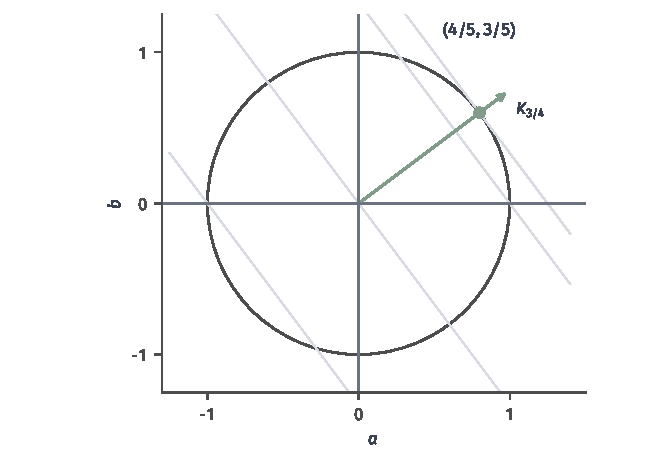
\includegraphics[width=112.0mm]{figures/01-mathematical-preliminaries-upper/02-linear-algebra-and-geometry/matplotlib/teaching-analysis/functional-affine-point-readout.pdf}
 \functionalinlinefigurecaption{fig:functional-affine-point-readout}
   {仿射RKHS中读取$f(3/4)=a+3b/4$。灰圆表示$a^2+b^2\leq1$，绿箭头是核截面$K_{3/4}$对应的系数$(1,3/4)$；灰平行线为相同点值。绿圆点$(4/5,3/5)$达到单位范数球上的最大点值$5/4$。这里坐标是函数系数，不是输入位置。图为解析教学示例。}
\end{minipage}
\end{center}

在实轴上固定$\sigma>0$，定义高斯核
$K_\sigma(x,z)=\exp(-(x-z)^2/(2\sigma^2))$。它满足正定核条件，因为
\[
 K_\sigma(x,z)=
 e^{-x^2/(2\sigma^2)}e^{-z^2/(2\sigma^2)}
 \sum_{k=0}^{\infty}\frac{x^kz^k}{\sigma^{2k}k!};
\]
每个有限部分和都是特征内积核，有限Gram二次型取极限仍非负。

上面的推导从函数空间得到核。反方向同样成立，而且不需要输入域带有拓扑或测度\scite{aronszajn1950kernels}。

\begin{theorem}[正定核的RKHS构造]
\label{thm:functional-moore-aronszajn-construction}
设$\mathcal{X}$为任意非空集合，$K:\mathcal{X}\times\mathcal{X}\to\mathbb{R}$
对称，并满足定义~\ref{def:functional-positive-definite-kernel}中的有限半正定条件。则存在
唯一的函数RKHS $\mathcal{H}_K$以$K$为再生核；这里的唯一性指保持每个函数不变的
等距同构。
\end{theorem}

\begin{proof}
先令$\mathcal{V}_0$为核截面符号$K_x$的形式有限线性组合所成的向量空间：
\[
  \mathcal{V}_0
  =
  \left\{
    \sum_{i=1}^{n}a_iK_{x_i}:
    n\in\mathbb{N},\
    a_i\in\mathbb{R},\
    x_i\in\mathcal{X}
  \right\}.
\]
这里的$K_x$暂时只是由$x$索引的形式符号，尚未把不同形式和按逐点函数值识别。
对
$f=\sum_i a_iK_{x_i}$和$g=\sum_jb_jK_{z_j}$定义
\begin{equation}
  \langle f,g\rangle_0
  =
  \sum_{i,j}a_i b_jK(x_i,z_j).
  \label{eq:functional-kernel-pre-inner-product}
\end{equation}
正定性只保证$\langle f,f\rangle_0\geq0$，还可能有非零形式和的长度为零。令
\[
  \mathcal{N}
  =
  \{f\in\mathcal{V}_0:\langle f,f\rangle_0=0\}.
\]
半内积仍满足Cauchy--Schwarz不等式：对
$\langle g,g\rangle_0>0$，最小化非负二次式
$\langle f-tg,f-tg\rangle_0$即可得到原来的证明；
若$\langle g,g\rangle_0=0$，非负式
$\langle f+tg,f+tg\rangle_0=\langle f,f\rangle_0+2t\langle f,g\rangle_0$
对所有实数$t$成立，迫使交叉项为零。
因此$f\in\mathcal{N}$时$\langle f,g\rangle_0=0$对所有$g$成立。
这又说明$\mathcal N$是线性子空间，且改变代表元只增加与所有元素正交的项。
所以可以商掉$\mathcal{N}$，使式
\eqref{eq:functional-kernel-pre-inner-product}成为真正的内积。

还需证明这个商空间能够忠实地解释为函数。对形式和
$f=\sum_i a_iK_{x_i}$，定义
\[
  (Jf)(x)
  =
  \sum_i a_iK(x,x_i)
  =
  \langle f,K_x\rangle_0.
\]
若$f\in\mathcal{N}$，则
\[
  |(Jf)(x)|^2
  =
  |\langle f,K_x\rangle_0|^2
  \leq
  \langle f,f\rangle_0K(x,x)
  =0,
\]
所以$Jf$处处为零。反过来，若$Jf$处处为零，则
\[
  \langle f,f\rangle_0
  =
  \sum_i a_i(Jf)(x_i)
  =0,
\]
故$f\in\mathcal{N}$。因此$\ker J=\mathcal{N}$，商空间
$\mathcal{H}_0=\mathcal{V}_0/\mathcal{N}$可单射地识别为函数空间，并且其中的
函数满足
\[
  f(x)=\langle f,K_x\rangle_0.
\]

对这个内积空间作完备化，得到Hilbert空间$\mathcal{H}_K$。还要确认完备化后的抽象极限
仍是函数。若$(f_m)\subset\mathcal{H}_0$在核范数下为柯西序列，则对每个$x$，
\[
  |f_m(x)-f_\ell(x)|
  \leq
  \lVert f_m-f_\ell\rVert_0\sqrt{K(x,x)},
\]
所以$(f_m(x))$是实数柯西序列。定义$f(x)=\lim_m f_m(x)$。若另一个柯西序列与
$(f_m)$表示同一个完备化元素，同一不等式保证两者逐点极限相同。故完备化元素具有
良定义的函数值，且内积连续性给出
\[
  f(x)
  =
  \lim_m\langle f_m,K_x\rangle_0
  =
  \langle f,K_x\rangle_{\mathcal{H}_K}.
\]
再生性质因此延伸到整个$\mathcal{H}_K$。这个逐点解释在完备化后仍是单射：若
$f\in\mathcal{H}_K$处处取零，则$f$与每个$K_x$正交；核截面的线性张成
$\mathcal{H}_0$在其完备化$\mathcal{H}_K$中稠密，所以$f$与整个空间正交，只能有
$f=0$。

唯一性也由这个构造确定。若另一个RKHS $\widetilde{\mathcal{H}}$也以$K$为核，则有限核截面和
在两个空间中的内积都由式
\eqref{eq:functional-kernel-pre-inner-product}决定。核截面的线性张成在任一空间中
都稠密；否则与所有$K_x$正交的函数$f$满足$f(x)=0$对所有$x$成立，只能是零函数。
所以有限核截面和之间的恒等映射唯一地延伸为两个完备空间之间的等距同构。
\end{proof}

定理\ref{thm:functional-moore-aronszajn-construction}说明，验证所有有限Gram矩阵半正定
就足以定义一个RKHS。它不同于Mercer谱展开。后者通常还假设$\mathcal{X}$是紧空间、
$K$连续，并选定具有适当支持的有限测度；这些条件使积分算子
\[
  (T_Kf)(x)
  =
  \int_{\mathcal{X}}K(x,z)f(z)\,\mathrm{d}\mu(z)
\]
成为紧自伴算子，从而可以用特征值与特征函数展开$K$。一般正定核即使不满足这些拓扑和
测度条件，仍有上述RKHS构造。因而，核的合法性、核的谱展开以及谱展开的一致收敛是三项
条件不同的结论。

反过来，稳定点值也不强迫函数关于输入连续。在$[-1,1]$上固定
$q(x)=\mathbb I\{x>0\}$，空间$\{a q:a\in\mathbb R\}$配内积
$\langle aq,bq\rangle=ab$就是一个RKHS：$|aq(x)|\leq|a|$，但非零元素有跳跃。
这个跳跃函数空间的核为$K(x,z)=q(x)q(z)$，可直接核验再生性质。

要比较算子输出与某个测试方向的内积，需要把这个测试方向变换到输入空间。
\begin{definition}[Hilbert空间之间的伴随算子]
\label{def:functional-adjoint}
设$\mathcal H,\mathcal G$为实Hilbert空间，$S:\mathcal H\to\mathcal G$为有界线性算子，
即存在有限$C\geq0$使$\lVert Sf\rVert_{\mathcal G}\leq C\lVert f\rVert_{\mathcal H}$。
其伴随是满足
\[
 \langle Sf,g\rangle_{\mathcal G}
 =\langle f,S^*g\rangle_{\mathcal H}
 \quad(f\in\mathcal H,\ g\in\mathcal G)
\]
的有界线性算子$S^*:\mathcal G\to\mathcal H$。
\end{definition}
对固定$g$，左边是关于$f$的有界线性泛函，Riesz表示给出唯一的$S^*g$；
表示元的唯一性又保证$S^*$线性，且$\lVert S^*g\rVert_{\mathcal H}\leq C\lVert g\rVert_{\mathcal G}$。
因此伴随确实存在且唯一。它把内积中的算子换到另一侧，并不要求$S$可逆。
在有限维实正交坐标中，伴随对应矩阵转置；在复正交坐标中，相应的复伴随对应共轭转置。
后面的Mercer证明会用伴随把两个函数空间中的内积联系起来。

一个可以直接核验的例子是$A:L^2(0,1)\to L^2(0,1)$，
$(Af)(x)=\int_0^x f(t)\,\mathrm dt$。Cauchy--Schwarz给出
$|Af(x)|^2\leq x\lVert f\rVert_2^2$，所以$\lVert A\rVert_{\mathrm{op}}\leq1/\sqrt2$。
交换三角区域中的积分可得
\[
 \langle Af,g\rangle
 =\int_0^1 f(t)\left(\int_t^1g(x)\,\mathrm dx\right)\mathrm dt,\qquad
 (A^*g)(t)=\int_t^1g(x)\,\mathrm dx.
\]
例如$A1(x)=x$，而$A^*1(t)=1-t$。伴随把输出测试的累积权重送回输入，
并不把$Af$反解成$f$，也不一定等于$A$自身。

\begin{definition}[自伴、正与紧算子]
\label{def:functional-operator-properties}
设$T:\mathcal H\to\mathcal H$为实Hilbert空间上的有界线性算子。若对所有$f,g\in\mathcal H$
有$\langle Tf,g\rangle=\langle f,Tg\rangle$，称$T$自伴，即$T^*=T$。
若$T$自伴且$\langle Tf,f\rangle\geq0$对每个$f\in\mathcal H$成立，称$T$为正算子。
若对每个有界序列$(f_n)$，序列$(Tf_n)$都具有在$\mathcal H$中范数收敛的子列，称$T$为紧算子。
\end{definition}
紧性也可用于$S:\mathcal H\to\mathcal G$，此时要求有界输入序列的像在
$\mathcal G$中有范数收敛子列，不要求两个空间相同。
自伴与正性则必须在同一Hilbert空间上比较$T$与$T^*$或$\langle Tf,f\rangle$。
有界性只控制输出大小，紧性还要求输出序列能抽出稳定的近似方向。在无限维
$\ell^2$中，恒等算子有界、自伴且为正，却不紧：标准单位向量序列经过它仍然
两两相距$\sqrt2$，没有收敛子列。后面的有限秩逼近正是建立紧性的途径。

\subsection{函数的积分变换}
\label{sec:functional-integral-transforms}
\label{sec:functional-kernel-spectrum-regularization}

有限Gram矩阵只访问有限个位置。要考察核如何作用于整个函数，需要先指定积分测度，
再把核值累计成新的函数；这个积分算子的谱才描述全域作用。给定测度空间
$(\mathcal X,\mu)$，假设$\mu$为$\sigma$有限测度，即$\mathcal X$可由可数个
有限测度可测集覆盖。对可测平方可积核$K\in L^2(\mu\otimes\mu)$，定义
\begin{equation}
 (T_Kf)(x)=\int_{\mathcal X}K(x,z)f(z)\,\mathrm d\mu(z).
 \label{eq:functional-kernel-integral-operator}
\end{equation}
Fubini定理保证几乎所有$x$的核截面属于$L^2(\mu)$，故积分几乎处处存在。
Cauchy--Schwarz进一步给出
\[
 |T_Kf(x)|^2
 \leq\left(\int|K(x,z)|^2\,\mathrm d\mu(z)\right)\lVert f\rVert_2^2,\qquad
 \lVert T_Kf\rVert_2\leq\lVert K\rVert_{L^2(\mu\otimes\mu)}\lVert f\rVert_2.
\]
所以输出确实属于$L^2$，且
$\lVert T_K\rVert_{\mathrm{op}}\leq\lVert K\rVert_{L^2(\mu\otimes\mu)}$。
核在零测集上的修改不影响该算子。

$T_K$还是紧算子。把$K$在
$L^2(\mu\otimes\mu)$中用有限个矩形指示函数的线性组合逼近，相应积分算子只有有限维
值域。例如$K_N(x,z)=\sum_{j=1}^N a_j\mathbb I_{A_j}(x)\mathbb I_{B_j}(z)$，
其中集合测度有限，则$T_{K_N}f$落在$\{\mathbb I_{A_j}\}$的张成空间。
这里需要的不是任意简单函数，而是矩形指示函数的有限和。先限制到有限测度块
$E\times E$。有限矩形并形成一个生成乘积$\sigma$代数的集合代数。
能在对称差测度下被该代数任意逼近的集合，对补集和有限并封闭；
对可数并，先用有限并截断，再用有限测度的下连续性控制余下部分，故也封闭。
所以块内每个可测集都能这样逼近。又因
$\lVert\mathbb I_A-\mathbb I_B\rVert_2^2=(\mu\otimes\mu)(A\mathbin\triangle B)$，
这种集合逼近给出指示函数的$L^2$逼近，再与简单函数逼近结合即可逼近任意平方可积核。
最后由$\sigma$有限性选递增的有限测度集$E$覆盖$\mathcal X$，
核在$E\times E$外的平方积分趋于零，于是得到全空间上的矩形和逼近。
上面的估计使$\lVert T_K-T_{K_N}\rVert_{\mathrm{op}}\to0$。
有限秩算子把有界序列送入有限维有界集；逐个抽取子列并作对角选择，
再用一致算子范数误差，就得到$T_Kf_n$的柯西子列。输出空间完备，故该子列收敛，
这说明有限秩算子的范数极限确实紧。

对称性$K(x,z)=K(z,x)$几乎处处成立时，交换积分给出$T_K^*=T_K$；
绝对可积性由$K\in L^2(\mu\otimes\mu)$和$(x,z)\mapsto f(z)g(x)\in L^2$
保证。正性还要另查。若$K$有处处有限、可测的正定核代表，则$T_K$为正：
先把$f$限制在有限测度集$E$上，并令$|f|$及$K(x,x)$在$E$上有界。
对$n\geq2$，将有限半正定不等式
$\sum_{i,j=1}^n f(x_i)f(x_j)K(x_i,x_j)\geq0$在$E^n$上积分，
对$\mu(E)>0$除以$n\mu(E)^{n-2}$，得到
\[
 (n-1)\int_{E\times E}f(x)K(x,z)f(z)\,\mathrm d\mu(x)\mathrm d\mu(z)
 +\mu(E)\int_E f(x)^2K(x,x)\,\mathrm d\mu(x)\geq0.
\]
除以$n-1$并令$n\to\infty$，双积分非负。由$\sigma$有限性可选递增的这类截断集
覆盖$\mathcal X$；$f\mathbb I_E\to f$于$L^2$，有界性将结论传给任意$f$。
这里没有把算子正性与核处处正定性混同：算子忽略零测集，任意修改零测集上的核值
可能破坏某个有限Gram矩阵，却不改变算子。

有些函数经积分变换后只改变幅度，不改变形状。
若非零函数$h$满足$Th=\lambda h$，就称它为特征方向，$\lambda$为对应特征值。
其中$\lambda=0$表示这个函数方向被完全消去；反求时不能对它取正特征值倒数。


\begin{theorem}[紧自伴算子的正交分解]
\label{thm:functional-compact-selfadjoint-spectrum}
设$T$为实Hilbert空间上的紧自伴算子。
其非零特征空间有限维，不同特征值的方向正交；
非零特征值可列成有限或可数序列，无限时趋于零。
这些特征方向与$\ker T$的闭张成等于整个空间，且
$Tf=\sum_j\lambda_j\langle f,e_j\rangle e_j$在空间范数下成立。
\end{theorem}
\begin{proof}
自伴性给出$(\lambda-\nu)\langle u,v\rangle=0$，故不同特征值的方向正交。
$T=0$时结论直接成立，以下设$T\neq0$。令$q=\sup_{\lVert x\rVert=1}|\langle Tx,x\rangle|$。
极化公式使单位$x,y$满足
$|\langle Tx,y\rangle|\leq q(\lVert x+y\rVert^2+\lVert x-y\rVert^2)/4=q$，
所以$\lVert T\rVert=q>0$。选取单位$x_n$，使其二次型沿一个子列趋于
$\lambda=\lVert T\rVert$或$-\lVert T\rVert$。于是
\[
 \lVert Tx_n-\lambda x_n\rVert^2
 \leq\lVert T\rVert^2-2\lambda\langle Tx_n,x_n\rangle+\lambda^2\to0.
\]
紧性使$Tx_n$有收敛子列，$\lambda\neq0$使相应$x_n$也收敛到单位$x$，
且$Tx=\lambda x$。非零特征空间若无限维，就可取无穷正交单位方向，
其像彼此距离为$\sqrt2|\lambda|$，违背紧性，故该空间有限维。

取这个特征空间的正交补。自伴性使其对$T$不变，可以在限制算子上重复上述构造，
每次取出其最大绝对特征值的整个有限维空间。
若过程无限且这些绝对值不趋零，对应正交单位特征向量的像没有柯西子列，
仍与紧性矛盾。因此余下限制算子的范数趋零。
所有已取方向的共同正交补上的作用于是为零；有限终止时也只有零限制才能终止。
投影定理将任意$f$分解为这些方向的闭张成分量与零空间分量，
正交展开及算子范数尾界给出所述级数。反过来零空间与每个非零特征方向正交。
\end{proof}
这里的谱分解把算子作用写成各个正交特征方向上的伸缩。定理说明，$T_K$的非零
特征值都是实数且重数有限；若非零特征值无限多，它们
只能聚集到$0$。相应特征向量与零空间的闭线性张成等于整个Hilbert空间；换言之，一般
元素可分解为一个零空间元素与非零特征方向上的范数收敛级数之和。这个结论给出$L^2(\mu)$中的算子谱，
却还没有保证核本身在每个$(x,z)$处都等于特征函数级数\scite{math-conway1990functional}。

Mercer定理补上点态展开所需的条件。有限Gram矩阵$[K(x_i,x_j)]_{i,j}$只记录有限个输入之间的关系；
积分算子的谱则依赖整个输入空间及其测度。下面用全支撑测度保证连续函数信息不会被
积分忽略；否则积分谱可能看不见某个非空开区域中的核信息。
这里“可分空间”指存在可数稠密子集；紧度量空间的可分性使下面的展开可以用一个可数序列
记录，而非假设所有无限维空间天然都有可数基。

\begin{example}[同一个核在两种内积下的坐标]
\label{ex:functional-affine-mercer-coordinates}
沿用例~\ref{ex:functional-affine-rkhs}的仿射核$K(x,z)=1+xz$，在$[-1,1]$上增加
测度$\mathrm d\mu(x)=\mathrm dx/2$。核已经固定了RKHS内积；测度另行决定$L^2(\mu)$
内积。因为$\int x\,\mathrm d\mu(x)=0$、$\int x^2\,\mathrm d\mu(x)=1/3$，
同一个函数$f(x)=a+bx$的两种长度为
\begin{equation}
 \begin{aligned}
  \lVert f\rVert_{\mathcal H_K}^2&=a^2+b^2,\\
  \lVert f\rVert_{L^2(\mu)}^2
  &=\int_{-1}^1(a+bx)^2\frac{\mathrm dx}{2}
    =a^2+\frac{b^2}{3}.
 \end{aligned}
 \label{eq:functional-affine-two-norms}
\end{equation}
因此$h_1(x)=1$、$h_2(x)=x$是RKHS中的标准正交基，而在$L^2(\mu)$中，同样两个
方向要写成$\psi_1(x)=1$、$\psi_2(x)=\sqrt3x$才能归一化。

积分算子的作用也可直接计算。对任意$g\in L^2(\mu)$，
\[
 (T_Kg)(x)=\int g(z)\,\mathrm d\mu(z)
             +x\int zg(z)\,\mathrm d\mu(z).
\]
代入$\psi_1,\psi_2$，得到$T_K\psi_1=\psi_1$、$T_K\psi_2=\psi_2/3$，
所以正特征值为$\mu_1=1$、$\mu_2=1/3$。其余与$1,x$都正交的函数被送到零，
属于算子的零空间。核展开于是为
\[
 K(x,z)=1+\frac13(\sqrt3x)(\sqrt3z)=1+xz.
\]
这里$\psi_1,\psi_2$只张成$L^2(\mu)$中的仿射函数子空间，不是整个$L^2(\mu)$的基。
包含映射$S:\mathcal H_K\to L^2(\mu)$保持函数值，即$Sf=f$，却不保持范数：
$Sh_1=\psi_1$、$Sh_2=\psi_2/\sqrt3$。在两边各自的归一化坐标中，
它将第二个方向的长度缩为$1/\sqrt3$。
\end{example}

\begin{center}
\begin{minipage}{\linewidth}
 \centering\small
 \begin{tabularx}{\linewidth}{@{}lXX@{}}
 \toprule
 比较对象 & RKHS $\mathcal H_K$ & $L^2(\mu)$\\
 \midrule
 $f(x)=a+bx$的范数平方 & $a^2+b^2$ & $a^2+b^2/3$\\
 常数方向，$\mu_1=1$ & $h_1(x)=1$ & $\psi_1(x)=1$\\
 线性方向，$\mu_2=1/3$ & $h_2(x)=x$ & $\psi_2(x)=\sqrt3x$\\
 \bottomrule
 \end{tabularx}
 \functionalinlinetablecaption{tab:functional-affine-mercer-coordinates}
   {仿射核在RKHS与$L^2(\mathrm dx/2)$中的尺度对照。两列分别按各自内积归一化；
   表中只列出积分算子的两个正特征方向。}
\end{minipage}
\end{center}

这个例子把核、积分测度和特征函数联系起来。一般的连续正定核也能这样展开，但需要
把有限个方向的分解推广为级数，并保证核值在整个输入域上得到一致控制。
\begin{theorem}[连续正定核的Mercer展开]
\label{thm:functional-mercer}
设$\mathcal{X}$为非空紧度量空间，$\mu$为有限、全支撑Borel测度，即每个非空开集
都有正测度。设$K:\mathcal{X}\times\mathcal{X}\to\mathbb{R}$连续、对称，且对任意
有限输入组满足正定核的半正定条件。则$T_K$是$L^2(\mu)$上的紧、自伴、正算子。
其正特征值按重数记为$(\mu_j)$，可为有限个或可数无穷个；相应特征函数可选为连续的
$L^2(\mu)$标准正交函数$(\psi_j)$，并有
\begin{equation}
 K(x,z)=\sum_{j:\mu_j>0}\mu_j\psi_j(x)\psi_j(z).
 \label{eq:functional-mercer-expansion}
\end{equation}
级数在$\mathcal{X}\times\mathcal{X}$上绝对且一致收敛，且
$\sum_j\mu_j=\int K(x,x)\,\mathrm d\mu(x)<\infty$。
若$K\equiv0$，右侧为空和。$T_K$可能另有零空间，零特征值不进入这个展开。
\end{theorem}

\begin{proof}
证明的关键是先在RKHS中分解，再用连续性把逐点结论加强为一致结论。
由前面的Moore--Aronszajn构造得到$\mathcal H_K$。核连续意味着
\[
 \lVert K_x-K_z\rVert_{\mathcal H_K}^2
 =K(x,x)+K(z,z)-2K(x,z)\longrightarrow0\quad(z\to x),
\]
所以每个$f\in\mathcal H_K$连续。紧度量空间有可数稠密子集，其核截面的张成在
$\mathcal H_K$中稠密：任意$K_x$都可用稠密子集的核截面依上面的范数连续性逼近，
而全部核截面的张成已知稠密。再把有限组合的系数取为有理数，
就得到可数稠密集合，故该空间可分；这使下面的标准正交基和级数可以按可数指标列出。

令$S:\mathcal H_K\to L^2(\mu)$为包含映射$Sf=f$。点值上界保证
$\lVert Sf\rVert_{L^2}^2\leq\lVert f\rVert_{\mathcal H_K}^2\int K(x,x)\,\mathrm d\mu(x)$。
若$Sf=0$，连续函数$f$几乎处处为零；全支撑性排除了非零连续函数只在一个零测开区域
出现的可能，故$f=0$，即$S$单射。取$\mathcal H_K$的标准正交基$(e_j)$，再生性质和
Parseval等式给出
\[
 \begin{aligned}
 \sum_j\lVert Se_j\rVert_{L^2}^2
 &=\int\sum_j|e_j(x)|^2\,\mathrm d\mu(x)\\
 &=\int\lVert K_x\rVert_{\mathcal H_K}^2\,\mathrm d\mu(x)
 =\int K(x,x)\,\mathrm d\mu(x)<\infty.
 \end{aligned}
\]
非负积分与求和的交换由单调收敛保证。这一有限尾和可以直接控制有限秩逼近：
将输入投影到前$N$个基方向所得的有限秩算子逼近$S$，算子范数误差平方不超过上述级数
的尾和，所以$S$紧。

用Riesz表示定义伴随$S^*$。对$g\in L^2(\mu)$，再生性质给出
\[
 (S^*g)(x)=\langle S^*g,K_x\rangle_{\mathcal H_K}
 =\langle g,SK_x\rangle_{L^2}
 =\int g(z)K(z,x)\,\mathrm d\mu(z),
\]
因而$SS^*=T_K$。这也直接核对了$T_K$的正性。
在例~\ref{ex:functional-affine-mercer-coordinates}中，$S$的归一化坐标矩阵为
$\operatorname{diag}(1,1/\sqrt3)$，伴随在这两个方向上具有同样的反向坐标矩阵；
$S^*S$与$SS^*$便分别在两个空间中具有特征值$1,1/3$。
一般情形也通过这两个组合算子联系两边的特征方向。
紧正算子$S^*S$没有零特征方向，故其标准正交特征向量$(h_j)$构成
$\mathcal H_K$的基。设相应正特征值为$\mu_j$，令
$\psi_j=Sh_j/\sqrt{\mu_j}$。于是$\psi_j$连续且在$L^2(\mu)$中标准正交，
$T_K\psi_j=\mu_j\psi_j$。反向地，$T_K$的任意正特征方向通过$S^*$对应到
$S^*S$的同特征值方向，所以没有遗漏正特征值。对$K_x,K_z$在$(h_j)$中应用Parseval等式，得到
\[
 K(x,z)=\sum_j h_j(x)h_j(z)
       =\sum_j\mu_j\psi_j(x)\psi_j(z).
\]
特别地，对角展开的余项
$r_N(x)=K(x,x)-\sum_{j\leq N}\mu_j\psi_j(x)^2$连续、非负，并逐点单调降到零。
给定$\varepsilon>0$，开集$\{x:r_N(x)<\varepsilon\}$随$N$增加，且覆盖紧空间；
有限子覆盖保证某一个$N$已覆盖全部空间，因此$r_N$一致趋于零。Cauchy--Schwarz
不等式进一步给出
\[
 \sum_{j>N}|\mu_j\psi_j(x)\psi_j(z)|
 \leq\sqrt{r_N(x)r_N(z)}\longrightarrow0
 \quad\text{一致于 }(x,z).
\]
这同时证明绝对收敛及一致收敛。对对角展开积分并用标准正交性，可得
$\int K(x,x)\,\mathrm d\mu(x)=\sum_j\mu_j$。零核的情形直接成立。
\end{proof}

上述证明把两项条件的作用分开了：全支撑性保证连续函数的$L^2$等价类没有隐藏的非零区域，
紧致性将连续的递减余项从逐点控制提升为统一控制。紧自伴算子谱、Mercer点态展开与有限
Gram矩阵分解因此是三个层次的结论，不能仅从有限矩阵的半正定性推断全域的一致展开\scite{mercer1909functions}。

在上述Mercer条件下，$\mu_j>0$的方向构成相应RKHS的谱坐标。函数可写成
$f=\sum_jb_j\psi_j$，其范数为
\begin{equation}
  \lVert f\rVert_{\mathcal{H}_K}^2
  =
  \sum_{j:\mu_j>0}\frac{b_j^2}{\mu_j}.
  \label{eq:functional-rkhs-spectral-norm}
\end{equation}
这个式子不仅是形式记号。证明中$h_j=\sqrt{\mu_j}\psi_j$是$\mathcal H_K$的
正交归一基；写$f=\sum_j a_jh_j$，便有$b_j=a_j\sqrt{\mu_j}$，
Parseval等式给出上述范数。反过来，只要$\sum_j b_j^2/\mu_j<\infty$，
相应级数就在$\mathcal H_K$中收敛，从而给出合法函数，并逐点收敛到该函数；
由于紧域上核对角有界，这里还一致收敛。
仅有$\sum_j b_j^2<\infty$只保证$L^2$成员资格，不足以保证属于RKHS。
$L^2$零特征方向不在此展开中，不能对零特征值取倒数。
小正特征值对应更昂贵的核范数方向；这种尺度怎样影响最优解，接下来在优化中计算。

回到例~\ref{ex:functional-affine-mercer-coordinates}，$f(x)=a+bx$在$L^2(\mu)$
归一化方向中的系数为$b_1=a$、$b_2=b/\sqrt3$。式
\eqref{eq:functional-rkhs-spectral-norm}将第二个系数的平方除以$\mu_2=1/3$，
恢复$a^2+b^2$，与表~\ref{tab:functional-affine-mercer-coordinates}中的核范数一致。
小特征值在这里补偿的是两种归一化的尺度差异。更换积分测度会改变特征值和特征函数，
但不会改变已固定的核范数。


前面的核积分按输入位置累积函数值。若现在希望输入经某种对称变换后输出不变，
我们可以沿用第~\ref{sec:geometry-equivalence-relations}节的群作用，
把同一轨道上的函数值平均。有限群只需有限求和，因此先从这一情形验证。
\begin{theorem}[有限群平均的不变性]
\label{thm:geometry-finite-group-average}
对有限群$G$及任意实函数$h:\mathcal X\to\mathbb R$，定义
\begin{equation}
 \overline h(x)=\frac1{|G|}\sum_{g\in G}h(g\cdot x).
 \label{eq:geometry-finite-group-averaging}
\end{equation}
则$\overline h$对给定作用不变。
\end{theorem}
\begin{proof}
固定$a\in G$，由作用的复合条件，
\[
 \overline h(a\cdot x)=\frac1{|G|}\sum_{g\in G}h((ga)\cdot x).
\]
映射$g\mapsto ga$是$G$上的双射，其逆为$g\mapsto ga^{-1}$。
更换求和索引后右端等于$\overline h(x)$，结论对任意$a,x$成立。
\end{proof}

把有限求和换成均匀角度积分，就能处理连续旋转。对连续实函数$h$，
二维旋转群$\mathrm{SO}(2)$给出
\[
 \overline h(\bm x)=\frac1{2\pi}\int_0^{2\pi}
 h(\bm R(\theta)\bm x)\,\mathrm d\theta.
\]
把输入先旋转$\beta$，被积函数变成$h(\bm R(\theta+\beta)\bm x)$。
角度换元只移动积分区间，而函数以$2\pi$为周期，所以平均值不变。
这里的均匀角度权重，是有限群中每个元素权重相同的连续版本。

更一般的推广使用拓扑群，即群乘法和取逆都是连续映射的群。
这里还采用Hausdorff条件：任意两个不同元素具有互不相交的开邻域。
紧Hausdorff拓扑群上的归一化Haar测度（Haar measure）是对左右群平移都不变的概率测度；
对可积的$g\mapsto h(g\cdot x)$，这种不变性允许作与上面相同的换元。
本章不展开一般Haar测度的存在性证明。紧致性在这里有实质作用：
若想对实轴上全部平移赋予同样权重，各区间$[k,k+1)$就必须质量相同；
质量为正会使总量无穷，质量为零则使全轴质量为零，均不可能得到概率测度。

平均的代价是信息丢失。例如对$\{\bm I,-\bm I\}$作用取$h(\bm x)=x_1$，
平均恒为零；它不仅忽略符号，也失去幅度信息。若任务要预测朝向，旋转平均后的标量
更无法承担原来的输出职责。有限数据增强只鼓励训练样本上的近似关系，
架构恒等式则在所声明作用和精确算术下成立；网格插值、边界及数值误差仍须另查。

\subsection{函数与场的微分运算}
\label{sec:functional-spatial-differentiation}
\label{sec:geometry-smoothness-geometric-operators}


经典导数要求逐点极限存在，会排除带尖点但整体仍然规则的函数。为了只保留积分运算真正
需要的变化信息，可以反过来要求分部积分恒等式成立：让导数先作用在光滑测试函数上，
再检验能否由另一个普通函数表示结果。测试函数用来探测局部变化，其紧支撑意味着它在
靠近区域边界处恒为零，因此不会引入边界项。
\begin{definition}[测试函数与局部可积性]
\label{def:functional-tests-local-integrability}
设$U\subseteq\mathbb R^d$开。函数$\varphi$的支撑是集合
$\{\bm x\in U:\varphi(\bm x)\neq0\}$在$\mathbb R^d$中的闭包。
$C_c^\infty(U)$由无限次连续可微、支撑为$U$内紧集的实函数组成。
空间$L^1_{\mathrm{loc}}(U)$由对每个紧集$K\subset U$满足
$\int_K|f|<\infty$的可测函数的几乎处处等价类组成。
\end{definition}
前一项让测试远离边界，后一项让与任何局部测试函数的积分有限；不要求$f$在整个$U$上可积。
\begin{definition}[弱导数]
\label{def:functional-weak-derivative}
设$U\subseteq\mathbb R^d$开，$f\in L^1_{\mathrm{loc}}(U)$。
取多重指标$\alpha=(\alpha_1,\ldots,\alpha_d)\in\mathbb{N}_0^d$，记
$|\alpha|=\sum_{j=1}^d\alpha_j$，
$D^\alpha=\partial_1^{\alpha_1}\cdots\partial_d^{\alpha_d}$。若存在
$g_\alpha\in L^1_{\mathrm{loc}}(U)$使每个
$\varphi\in C_c^\infty(U)$都满足
\begin{equation}
  \int_U f(\bm{x})D^\alpha\varphi(\bm{x})\,\mathrm{d}\bm{x}
  =
  (-1)^{|\alpha|}
  \int_U g_\alpha(\bm{x})\varphi(\bm{x})\,\mathrm{d}\bm{x},
  \label{eq:functional-weak-derivative}
\end{equation}
就称$g_\alpha$为$f$的$\alpha$阶\term{弱导数}（weak derivative），记为
$D^\alpha f$，按几乎处处等价理解。
\end{definition}
弱导数若存在，则在几乎处处意义下唯一。这里使用测试函数的区分性质：
局部可积函数$u$若对每个$\varphi\in C_c^\infty(U)$满足$\int_Uu\varphi=0$，
则$u$几乎处处为零。这个结论对任意维数都成立。为核验它，在$U$内取一个闭矩形盒，
对盒内任意小矩形，用各坐标上取值于$[0,1]$的光滑紧支撑函数之积逼近其指示函数。
控制收敛给出$u$在每个小矩形上的积分都为零。以$\nu(A)=\int_A|u|$作为盒内有限测度，
前面的矩形代数逼近论证说明，每个可测集$A$都能用有限矩形并$B$使$\nu(A\mathbin\triangle B)$任意小。
于是$|\int_Au-\int_Bu|\leq\nu(A\mathbin\triangle B)$，而$\int_Bu=0$，故$\int_Au=0$。
特别对$\{u>0\}$与$\{u<0\}$积分，得到盒内$u=0$
几乎处处。用可数个内部矩形盒覆盖$U$便得结论。取两种候选弱导数之差即可得到唯一性。
式\eqref{eq:functional-weak-derivative}把经典分部积分当作定义；
测试函数的紧支撑使边界项消失，因此这个定义本身不需要给$U$另加边界条件。

有了弱导数，就可以同时累计函数值与导数的平方误差。包含正阶导数时，这比只控制
$L^2$误差提出了更强的规则性要求；零阶空间仍然是$L^2$。
\begin{definition}[整数阶平方可积Sobolev空间]
\label{def:functional-sobolev-space}
设$U\subseteq\mathbb R^d$为开集，$m\in\mathbb N_0$。Sobolev空间
\[
  W^{m,2}(U)
  =
  \left\{
    f\in L^2(U):
    D^\alpha f\in L^2(U),\ |\alpha|\leq m
  \right\}
\]
配备范数
\begin{equation}
  \lVert f\rVert_{W^{m,2}(U)}^2
  =
  \sum_{|\alpha|\leq m}
  \lVert D^\alpha f\rVert_{L^2(U)}^2.
  \label{eq:functional-sobolev-norm}
\end{equation}
其中$D^0f=f$，所有导数均按弱导数理解，元素按几乎处处等价识别。
\end{definition}
当$U=(a,b)$为一维区间时，$W^{m,2}(a,b)$也常记作$H^m(a,b)$，式
\eqref{eq:functional-sobolev-norm}相应写成
\[
  \lVert f\rVert_{H^m(a,b)}^2
  =
  \sum_{r=0}^{m}
  \int_a^b|D^r f(x)|^2\,\mathrm{d}x.
\]
这里$m\in\mathbb{N}_0$，各阶导数都按上面的弱导数定义理解；非整数阶Sobolev空间需要
其他定义，不由这个有限求和给出。
例如一维函数$f(x)=|x|$在原点没有经典导数，但其一阶弱导数几乎处处等于
$\operatorname{sign}(x)$；在有界区间上，它仍属于$W^{1,2}$。尖点因而不会自动排除
积分意义下的平滑性。

在$(-1,1)$上把积分分成左右两段，可以直接核对这一弱导数：
\[
 \int_{-1}^1 |x|\varphi'(x)\,\mathrm dx
 =\int_{-1}^0\varphi(x)\,\mathrm dx-\int_0^1\varphi(x)\,\mathrm dx
 =-\int_{-1}^1\operatorname{sign}(x)\varphi(x)\,\mathrm dx.
\]
两侧在$0$处的边界项都为零，原点处任意指定的单个导数值也不会改变积分。
图~\ref{fig:functional-weak-derivative}将这两条函数并列：弱导数允许用一个几乎处处
确定的函数保存变化信息，而不要求补出尖点处不存在的经典导数。
\begin{fullwidth}
\begin{minipage}{\linewidth}
 \centering
 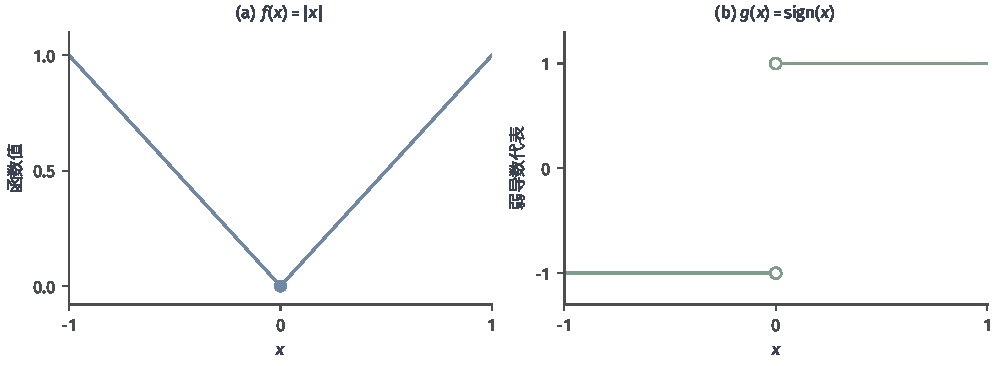
\includegraphics[width=169.0mm]{figures/01-mathematical-preliminaries-upper/02-linear-algebra-and-geometry/matplotlib/concepts-analysis-functional/weak-derivative.pdf}
 \functionalinlinefigurecaption{fig:functional-weak-derivative}
   {$f(x)=|x|$与其一阶弱导数$g(x)=\operatorname{sign}(x)$。左图原点为连续尖点；右图两段分别为$-1$与$1$，空心端点表示经典导数在原点未定义。弱导数在原点的代表值可以任取，积分恒等式不受影响。}
\end{minipage}
\end{fullwidth}

几乎处处存在经典导数仍不足以保证该导数就是弱导数。阶跃函数
$h(x)=\mathbb I\{x>0\}$几乎处处的经典导数为零，但
$\int_{-1}^1h\varphi'=-\varphi(0)$一般不为零。若能由某个局部可积函数$g$表示
它的弱导数，取支撑逐渐缩到原点、满足$0\leq\varphi_n\leq1$且$\varphi_n(0)=1$的
光滑测试函数，则$|\int g\varphi_n|\to0$，却应等于$1$，矛盾。因此跳跃与连续尖点
在弱导数意义下也有不同表现；单凭“只在一个点不可微”无法判断Sobolev成员资格。

$W^{m,2}(U)$的内积为
\[
 \langle f,g\rangle_{W^{m,2}}
 =\sum_{|\alpha|\leq m}\int_U D^\alpha f\,D^\alpha g.
\]
它诱导式~\eqref{eq:functional-sobolev-norm}的范数；其中包含零阶项，所以非零
元素的范数为正。证明完备性时，取其中的柯西列$(f_n)$。对每个
$|\alpha|\leq m$，序列$(D^\alpha f_n)$在$L^2(U)$中都是柯西列，故收敛到某个
$g_\alpha\in L^2(U)$，其中$g_0$记为$f$。把$f_n$的弱导数恒等式分别在两侧取极限；
Cauchy--Schwarz不等式保证与固定测试函数的积分连续，于是
\[
  \int_U fD^\alpha\varphi
  =
  (-1)^{|\alpha|}\int_U g_\alpha\varphi.
\]
因此$g_\alpha=D^\alpha f$，并且$f_n\to f$于
$W^{m,2}(U)$，所以这个空间确实是Hilbert空间。若另外要求边界条件，还须检查
可行子空间是否闭。例如定义
$W_0^{m,2}(U)=\overline{C_c^\infty(U)}^{\,W^{m,2}}$，由定义它是闭子空间，
因而仍为Hilbert空间；在具有适当边界规则性时，这才可进一步解释为相应的零边界条件。
不能在任意区域上不加说明地把“边界取零”套到几乎处处等价类上。

$L^2([0,1])$的元素只有几乎处处意义，单点值本来就未定义；即使只看连续代表，
第\ref{sec:functional-sequence-convergence}节的连续尖峰反例仍会否定点值不等式。
Sobolev空间则需要按阶数、维数与区域另行判断。例如在有限区间上，
$H^1(a,b)$的每个元素有唯一连续的绝对连续代表，其弱导数给出
$f(x)-f(t)=\int_t^x f'(s)\,\mathrm ds$。令$\ell=b-a$，对$t$平均并用
Cauchy--Schwarz可得
\[
 |f(x)|\leq \ell^{-1/2}\lVert f\rVert_{L^2}
              +\ell^{1/2}\lVert f'\rVert_{L^2}
 \leq\sqrt{\ell^{-1}+\ell}\,\lVert f\rVert_{H^1}.
\]
这里绝对连续代表的存在也能从弱导数恒等式得到。令$g=Df$，
$F(x)=\int_a^x g(s)\,\mathrm ds$，则$F$绝对连续且弱导数为$g$，
故$u=f-F$的弱导数为零。任取积分为零的$\eta\in C_c^\infty(a,b)$，
其原函数仍紧支撑，因而$\int u\eta=0$。固定积分为一的测试函数$\rho$，
把任意$\varphi$写成
$\varphi-(\int\varphi)\rho+(\int\varphi)\rho$，得到
$\int u\varphi=c\int\varphi$，其中$c=\int u\rho$。
局部可积函数若与所有光滑紧支撑测试函数的积分均为零，就几乎处处为零，
所以$u=c$几乎处处。这里所用的区分性质可以在一维直接验证：
对任意内部闭区间，用取值在$[0,1]$内的光滑紧支撑函数逼近其示性函数，
由控制收敛知该区间上的积分为零；因此不定积分在内部处处为常数，
再由Lebesgue积分的微积分基本定理得原函数几乎处处为零。
这给出$f$的绝对连续代表$F+c$；
两个连续代表若几乎处处相等，则处处相等。

因此选取这些连续代表后，$H^1(a,b)$可看作RKHS。维数改变后则可能失败。
例如在三维单位球$U$中取$\varphi\in C_c^\infty(U)$且$\varphi(0)=1$，
令$f_n(\bm x)=\varphi(n\bm x)$，其中$\varphi$在$U$外延拓为零。变量替换给出
\[
 \lVert f_n\rVert_{W^{1,2}(U)}^2
 =n^{-3}\lVert\varphi\rVert_2^2+
   n^{-1}\lVert\nabla\varphi\rVert_2^2\longrightarrow0,
 \qquad f_n(0)=1.
\]
所以即使只检验光滑函数，也不存在$|f(0)|\leq C\lVert f\rVert_{W^{1,2}(U)}$这样的统一界。
拥有弱导数不等于能稳定读取点值。


定义域若为第~\ref{chap:differential-geometry-and-symmetry}章的流形，标量函数仍可局部表达并求弱导数。
空间梯度$\operatorname{grad}f(p)$取值于$T_p\mathcal M$，
由式~\eqref{eq:geometry-riemannian-gradient-definition}表示输入位置的微分。
向量场的变化则用联络计算$\nabla_U V$；这避免把不同位置的坐标分量直接相减。
微分运算还要规定成员与边界行为。以下取紧致光滑Riemann流形，
无边界或具有Lipschitz边界；这里后者指在每个边界点附近，边界经坐标变换后是
某个Lipschitz函数的图像，允许闭点带这样的分片光滑边界及角点。
我们先对光滑函数作变分，再容纳有限能量极限：把光滑至边界的函数按下式范数完备化，
定义$H^1(\mathcal M)$，
\[
 \lVert f\rVert_{H^1}^2
 =\int_{\mathcal M}(|f|^2+\lVert\operatorname{grad}f\rVert_g^2)\,\mathrm dV_g.
\]
这个定义同时保留函数的$L^2$极限和梯度的$L^2$极限。
后一极限是弱梯度：它满足对任意内部光滑紧支撑向量场$\bm V$的恒等式
$\int g(\operatorname{grad}f,\bm V)\,\mathrm dV_g
=-\int f\operatorname{div}_g\bm V\,\mathrm dV_g$。
对光滑近似逐项分部积分并取极限，就得到这一关系；散度的坐标式在下面给出。
内积和体积均由度量定义，所以换坐标不改变这个关系。在欧氏坐标中，它还原为前面的弱导数。
这使有限能量但不逐点光滑的极限也可作为候选。
若在非紧空间工作，平方可积性、无穷远行为以及测试函数范围还须另定，
不能自动删去无穷远处的边界贡献。

第~\ref{sec:geometry-objects}节的开点带由
$\Phi(s,u)=((R+u)\cos(s/R),(R+u)\sin(s/R))$参数化，
其中$s\in(s_-,s_+)$、$|u|<w<R$且$s_+-s_-<2\pi R$。
开点带不含边界。需要固定边缘数值时，另取
\[
 \overline{\mathcal M}_{\mathrm{strip}}
 =\{\Phi(s,u):s\in[s_-,s_+],\ |u|\leq w\},
\]
沿用原参数式到闭区间的延拓。这是有分片光滑边界的紧积分域；
四个角点的法向虽不唯一，却是边界测度零集。
对光滑函数，边界值就是限制到$\partial\mathcal M$的函数；对$H^1$元素，
直接改动边界上的代表值并无意义，需要把这个限制运算连续延伸。
在上述Lipschitz边界条件下，光滑函数满足
$\lVert f|_{\partial\mathcal M}\rVert_{L^2(\partial\mathcal M)}
\leq C\lVert f\rVert_{H^1(\mathcal M)}$。
这项边界估计可在局部展平边界后，沿横向用一维积分估计，再将有限个局部估计相加得到。
因此光滑近似的边界值构成$L^2(\partial\mathcal M)$柯西列，其极限与近似选择无关。
这个极限定义有界线性迹映射
$\operatorname{Tr}:H^1(\mathcal M)\to L^2(\partial\mathcal M)$，
即有限能量函数的边界读数；本章不展开一般边界估计的证明。
零迹空间记为$H_0^1(\mathcal M)=\ker\operatorname{Tr}$，是闭子空间。
固定边界值时，允许扰动取自这个零迹空间；自由边界时，允许整个$H^1$中的扰动，
再由变分决定自然边界条件。

令$J_g=\sqrt{\det\bm G}$。光滑向量场
$\bm V=\sum_iV^i\partial_i$的散度为
\[
 \operatorname{div}_g\bm V
 =\frac1{J_g}\sum_i\partial_i(J_gV^i).
\]
它测量相对于几何体积的局部净流出：
对坐标小区域作普通分部积分时，$J_g$正是体积密度，
故不能只保留$\sum_i\partial_iV^i$。
其散度定理为
$\int_{\mathcal M}\operatorname{div}_g\bm V\,\mathrm dV_g
=\int_{\partial\mathcal M}g(\bm V,\bm n)\,\mathrm dS_g$，
其中$\bm n$在$T\mathcal M$内垂直于边界、指向外侧且为单位长度，
$\mathrm dS_g$是诱导边界面积元。

\begin{definition}[Laplace--Beltrami算子]
\label{def:geometry-laplace-beltrami}
设$f$为二阶连续可微的实函数。将梯度再取散度，得到
\term{Laplace--Beltrami算子}（Laplace--Beltrami operator）：
\begin{equation}
 \Delta_g f=\operatorname{div}_g(\operatorname{grad}f)
 =\frac1{\sqrt{\det\bm G}}\sum_{i,j}
  \frac{\partial}{\partial z^i}
   \left(\sqrt{\det\bm G}\,g^{i,j}
                   \frac{\partial f}{\partial z^j}\right).
 \label{eq:geometry-laplace-beltrami}
\end{equation}
其中$g^{i,j}$是逆度量矩阵$\bm G^{-1}$的第$(i,j)$项。
本章取$\Delta_g$为热方程生成元；适当边界条件下，$-\Delta_g$是非负算子。
\end{definition}
它描述相对于当前几何的局部二阶变化，不是任意坐标中的偏导平方和。
散度的乘积法则给出
$\operatorname{div}_g(h\operatorname{grad}f)
=g(\operatorname{grad}h,\operatorname{grad}f)+h\Delta_gf$。
积分并用散度定理，得到Green恒等式
\begin{equation}
 \int_{\mathcal M}g(\operatorname{grad}f,\operatorname{grad}h)\,\mathrm dV_g
 =-\int_{\mathcal M}h\Delta_gf\,\mathrm dV_g
   +\int_{\partial\mathcal M}h\,\partial_{\bm n}f\,\mathrm dS_g,
 \label{eq:geometry-green-identity}
\end{equation}
其中$\partial_{\bm n}f=g(\operatorname{grad}f,\bm n)$。

对向量场，$\nabla^*$是形式$L^2$伴随：先对光滑、紧支撑的测试场作分部积分，
把$\nabla$移到内积另一侧，得到相应的微分表达式。
这没有直接套用定义~\ref{def:functional-adjoint}中有界算子的伴随定理；
作为$L^2$中的微分算子，$\nabla$还需要另外规定可求导的定义域。
度量、联络和体积元决定形式表达式，函数空间与边界条件则进一步决定
实际算子及其Hilbert伴随的定义域。
算子$\nabla^*\nabla$称为联络拉普拉斯（connection Laplacian），本章取非负号约定。
在局部正交归一标架中，
\[
 \nabla^*\nabla\bm V
 =-\sum_a\left(\nabla_{\bm e_a}\nabla_{\bm e_a}\bm V
                 -\nabla_{\nabla_{\bm e_a}\bm e_a}\bm V\right).
\]
修正项记录标架自身的变化，不能省略。

Green恒等式也联系微分作用与谱，但必须先规定$-\Delta_g$在哪些函数上作用。
取能量空间$V$，无边界或齐次Neumann条件下令$V=H^1(\mathcal M)$，
齐次Dirichlet条件下令$V=H_0^1(\mathcal M)$。相应的$L^2$算子$A$定义为
\[
 \begin{aligned}
 D(A)&=\Bigl\{f\in V:\ \exists u\in L^2,\\
 &\qquad\int g(\operatorname{grad}f,\operatorname{grad}h)\,\mathrm dV_g
 =\int uh\,\mathrm dV_g\quad\forall h\in V\Bigr\},\\
 Af&=u.
 \end{aligned}
\]
测试空间$V$在$L^2$中稠密，所以$u$唯一。这个定义要求能量的一阶作用确实由
一个$L^2$函数表示；对光滑$f$，Green式给出$Af=-\Delta_gf$，并带有选定的边界条件。
下面使用这个非负自伴实现的标准椭圆谱结论，不在本章证明其一般形式。
在正维数、紧致、光滑且无边界的Riemann流形上，其定义域也可写为$H^2(\mathcal M)$，
即局部坐标中至二阶的弱导数平方可积的函数空间；$A$有离散谱
\[
 0=\lambda_0\leq\lambda_1\leq\cdots,\qquad\lambda_k\longrightarrow\infty,
\]
按重数排列，并有光滑特征函数组成完备正交系。
若$-\Delta_g\phi=\lambda\phi$且$\phi\neq0$，取$h=\phi$得到
\[
 \lambda\int_{\mathcal M}\phi^2\,\mathrm dV_g
 =\int_{\mathcal M}\lVert\operatorname{grad}\phi\rVert_g^2\,\mathrm dV_g
 \geq0.
\]
这证明非负性；离散性与完备性还使用紧致性和椭圆算子理论，不由此等式单独推出。
零特征函数在每个连通分支上为常量，连通时零特征空间恰为一维。
在有非空边界的连通紧光滑域上，Neumann条件仍保留常量零模，
齐次Dirichlet条件则使首个特征值严格为正；
若不是这类域，必须重新核对谱与边界条件，不能仅以“有边界”概括。


这里$-\Delta_g$通常是无界微分算子：在完整圆上对$\cos(n\theta)$作用，
其$L^2$放大率为$n^2/R^2$，没有对全部频率统一的有限算子界。
上述离散谱结论使用椭圆算子及其定义域条件，
不能把它当作定理~\ref{thm:functional-compact-selfadjoint-spectrum}对有界紧算子的直接应用。

\subsection{目标泛函的微分运算}
\label{sec:functional-objective-differentiation}

向量优化中的小位移在这里变为小函数扰动$h$，例如用$f+h$代替$f$。
设$J$在$f$的Hilbert空间开邻域内取有限实值。沿方向$h$的\term{方向导数}定义为
\[
 J'(f;h)=\lim_{t\to0}\frac{J(f+th)-J(f)}{t},
\]
前提是这个双侧极限存在。它只检查一条直线上的变化；要对所有足够小的扰动
使用同一个线性近似，还需要更强的条件。

\begin{definition}[函数泛函的Fréchet微分与梯度]
\label{def:functional-frechet-gradient}
设$\mathcal H$为实Hilbert空间，$J$在$f$的开邻域内取有限实值。
若存在有界线性泛函$DJ(f):\mathcal H\to\mathbb R$，使
\[
 J(f+h)=J(f)+DJ(f)[h]+r_f(h),\qquad
 \frac{|r_f(h)|}{\lVert h\rVert_{\mathcal H}}\longrightarrow0
 \quad(\lVert h\rVert_{\mathcal H}\to0),
\]
则称$J$在$f$处Fréchet可微，$DJ(f)$为其微分，也称\term{Fréchet导数}
（Fréchet derivative）。由Riesz表示，存在唯一
$\nabla_{\mathcal H}J(f)\in\mathcal H$满足
\[
 DJ(f)[h]=\langle\nabla_{\mathcal H}J(f),h\rangle_{\mathcal H}.
\]
这个空间元素称为相对于该内积的梯度。
\end{definition}
微分把一个扰动函数变成一阶目标变化，是有界线性读取；梯度则用空间里的一个方向
表示这项读取。Fréchet可微蕴含各方向导数存在且等于$DJ(f)[h]$，反过来未必成立。
例如在二维系数平面上令
$J(a,b)=a^3/(a^2+b^2)$（非零点），并令$J(0,0)=0$。
原点沿$(u,v)\neq0$的双侧方向导数为$u^3/(u^2+v^2)$，
它并非方向的线性函数：在$(1,0)$与$(0,1)$上的值之和为$1$，
在$(1,1)$上的值却为$1/2$，故不能作为Fréchet微分。

即使所有方向导数恰好组成有界线性泛函，仍可能缺少对方向的统一余项控制。
在同一个二维函数系数空间中定义
\[
 Q(a,b)=
 \begin{cases}
  \dfrac{a^3b}{a^4+b^2},&(a,b)\neq(0,0),\\
  0,&(a,b)=(0,0).
 \end{cases}
\]
由$2|a^2b|\leq a^4+b^2$得$|Q(a,b)|\leq|a|/2$，所以$Q$在原点连续。
对固定方向$(u,v)$，若$v=0$，则$Q(tu,tv)=0$；若$v\neq0$，则
$Q(tu,tv)/t=t u^3v/(t^2u^4+v^2)\to0$。
因此所有方向导数都为零，候选微分只能是零泛函。
但沿曲线$b=a^2$，有$Q(a,a^2)=a/2$，且
$|Q(a,a^2)|/\sqrt{a^2+a^4}\to1/2$，余项不满足Fréchet条件。
逐条直线上的极限不能代替对全部小扰动的统一线性近似。

对平方距离目标$J(f)=\frac12\lVert f-y\rVert_{\mathcal H}^2$，直接展开得到
\[
 J(f+h)-J(f)
 =\langle f-y,h\rangle_{\mathcal H}+\tfrac12\lVert h\rVert_{\mathcal H}^2.
\]
余项除以$\lVert h\rVert$趋于零，所以$DJ(f)[h]=\langle f-y,h\rangle$，
梯度为$f-y$。这里求的是目标对未知函数$f$的微分，不是$f(x)$对输入$x$的导数；
即使$y$有尖点，这个平方距离泛函仍然可微。

梯度还依赖内积的选择，而不只是目标的表达式。例如在仿射函数$f(x)=a+bx$上，
目标$J(f)=(a^2+b^2)/2$的微分始终是$DJ(f)[u+vx]=au+bv$。
用内积$ac+bd$时梯度是$a+bx$，改用$ac+4bd$时则为$a+(b/4)x$。
两个梯度表示相同的线性读取，但“最陡方向”所依据的长度不同。
若梯度非零，Cauchy--Schwarz表明单位范数方向中
$h=-\nabla_{\mathcal H}J(f)/\lVert\nabla_{\mathcal H}J(f)\rVert$
使$DJ(f)[h]$最小。这解释了梯度作为一阶下降方向的用途；
有限步更新能否降低目标，还要控制线性近似之外的余项。

\section{方程与优化}
\label{sec:functional-optimization-regularization}

前面已经能够比较、投影和读取函数，现在令函数本身成为未知量。
目标泛函$J$给每个候选函数一个评价值，问题写成
$\inf_{f\in C}J(f)$。$C=\mathcal H$表示没有额外可行约束，即使$J$中含有范数惩罚；
只有明确要求$f$属于某个较小集合$C$时，才增加可行约束。
以下以Hilbert空间及RKHS为主，不把结论直接推广到一般Banach空间。
下面先求最近函数，再分别处理有限读取与整体积分误差下的拟合，最后求解平滑能量问题。

\subsection{闭凸约束下的最近函数求解}
\label{sec:functional-nearest-function}

有限维最小二乘把观测向量投影到设计矩阵的列空间。
函数逼近的对应问题是：给定Hilbert空间$\mathcal H$中的目标$f$与候选集合$C$，
能否在$C$中取得最小距离？与有限维子空间不同，任意候选集合未必保留最小化序列的极限。
下面要求$C$非空、闭且凸，并用内积几何先证明近似最优候选构成柯西列，
再由完备性和闭性取得空间内、候选集合中的最近函数；同一个几何论证还给出唯一性。

\begin{theorem}[Hilbert空间投影定理]
\label{thm:functional-hilbert-projection}
设$\mathcal{H}$为实Hilbert空间，$C\subseteq\mathcal{H}$非空、闭且凸。对每个
$f\in\mathcal{H}$，存在唯一的$g^\star\in C$满足
\[
  \lVert f-g^\star\rVert_{\mathcal{H}}
  =\inf_{g\in C}\lVert f-g\rVert_{\mathcal{H}}.
\]
这个最近点由变分不等式
\begin{equation}
  \langle f-g^\star,g-g^\star\rangle_{\mathcal{H}}
  \leq0,\qquad g\in C
  \label{eq:functional-convex-projection-characterization}
\end{equation}
唯一刻画。若$C=M$是闭线性子空间，则该条件等价于
\begin{equation}
  f-g^\star\perp M.
  \label{eq:functional-subspace-projection-orthogonality}
\end{equation}
\end{theorem}

\begin{proof}
记$d=\inf_{g\in C}\lVert f-g\rVert_{\mathcal{H}}$，并取最小化序列
$(g_n)\subseteq C$，使$\lVert f-g_n\rVert_{\mathcal{H}}\to d$。凸性保证
$(g_n+g_m)/2\in C$。把平行四边形恒等式用于
$f-g_n$与$f-g_m$，得到
\begin{align*}
  \lVert g_n-g_m\rVert_{\mathcal{H}}^2
  &=
  2\lVert f-g_n\rVert_{\mathcal{H}}^2
  +2\lVert f-g_m\rVert_{\mathcal{H}}^2\\
  &\quad
  -4\left\lVert
    f-\frac{g_n+g_m}{2}
  \right\rVert_{\mathcal{H}}^2\\
  &\leq
  2\lVert f-g_n\rVert_{\mathcal{H}}^2
  +2\lVert f-g_m\rVert_{\mathcal{H}}^2-4d^2.
\end{align*}
右侧随$m,n\to\infty$趋于$0$，所以$(g_n)$是柯西序列。$\mathcal{H}$完备，故
$g_n\to g^\star\in\mathcal{H}$；$C$闭，故$g^\star\in C$。范数连续给出
$\lVert f-g^\star\rVert_{\mathcal{H}}=d$，存在性得证。

若$g_1,g_2\in C$都达到$d$，同一恒等式给出
\[
  \lVert g_1-g_2\rVert_{\mathcal{H}}^2
  =
  2d^2+2d^2
  -4\left\lVert f-\frac{g_1+g_2}{2}\right\rVert_{\mathcal{H}}^2
  \leq0,
\]
所以$g_1=g_2$。

再证明刻画。对任意$g\in C$和$t\in[0,1]$，凸性给出
$g^\star+t(g-g^\star)\in C$。最优性意味着
\[
  \lVert f-g^\star\rVert_{\mathcal{H}}^2
  \leq
  \lVert f-g^\star-t(g-g^\star)\rVert_{\mathcal{H}}^2.
\]
展开右侧、约去公共项并除以$t>0$，得到
\[
  2\langle f-g^\star,g-g^\star\rangle_{\mathcal{H}}
  \leq t\lVert g-g^\star\rVert_{\mathcal{H}}^2.
\]
令$t\downarrow0$便得到式
\eqref{eq:functional-convex-projection-characterization}。反过来，若该不等式成立，
则对任意$g\in C$，
\[
  \lVert f-g\rVert_{\mathcal{H}}^2
  =
  \lVert f-g^\star\rVert_{\mathcal{H}}^2
  +\lVert g-g^\star\rVert_{\mathcal{H}}^2
  -2\langle f-g^\star,g-g^\star\rangle_{\mathcal{H}}
  \geq
  \lVert f-g^\star\rVert_{\mathcal{H}}^2,
\]
所以$g^\star$是最近点。

若$C=M$为线性子空间，则对每个$h\in M$，可分别取
$g=g^\star+h$和$g=g^\star-h$。式
\eqref{eq:functional-convex-projection-characterization}同时给出
$\langle f-g^\star,h\rangle\leq0$与
$-\langle f-g^\star,h\rangle\leq0$，故内积为零。反向结论由勾股恒等式直接得到。
\end{proof}

闭性不能由“子空间”二字自动获得。以前面的$c_{00}\subset\ell^2$为例，目标
$\bm{a}=(1,1/2,1/3,\ldots)$到$c_{00}$的距离下确界为$0$，但$\bm{a}\notin c_{00}$，
所以不存在最佳逼近。有限截断可以任意接近目标，却没有一个有限截断达到距离$0$。


如果某些输入区域的误差更值得重视，可以在同一平方误差中改变权重，而不必改变候选空间。
设$w$是$[-1,1]$上可测、几乎处处为正且属于$L^1([-1,1])$的权重。在关于测度
$w(x)\,\mathrm{d}x$的几乎处处等价类所成空间
$L^2([-1,1],w(x)\,\mathrm{d}x)$上，定义
\[
  \langle f,g\rangle_w
  =
  \int_{-1}^{1}f(x)g(x)w(x)\,\mathrm{d}x.
\]
加权平方可积性与Cauchy--Schwarz不等式保证该积分对空间中任意$f,g$有限；权重几乎
处处为正则保证它确实定义内积。由于紧区间上的多项式有界，而$w$可积，每个多项式都属于
这个加权空间，因此可以对幂函数序列作Gram--Schmidt正交化。权重$w(x)=1$对应Legendre
多项式；权重$w(x)=(1-x^2)^{-1/2}$（端点值任取）对应第一类Chebyshev多项式
$T_j(x)=\cos(j\arccos x)$。后者在$x=\pm1$附近赋予更大权重，因此相同次数的投影
优化的是另一种积分误差。

具体地，给定线性无关的$\phi_0,\phi_1,\ldots$，依次令
\[
 q_j=\phi_j-\sum_{k<j}\langle\phi_j,e_k\rangle_w e_k,\qquad
 e_j=q_j/\lVert q_j\rVert_w.
\]
减去已有方向的投影后，$q_j$与这些方向正交；线性无关保证分母非零。
对$\phi_j(x)=x^j$使用该构造就得到归一化的正交多项式。

通常采用$P_j(1)=T_j(1)=1$的尺度约定，它们正交但一般并非单位长度。
下面两组递推均从$j\geq1$开始。这一约定下，Legendre多项式满足
\[
  P_0(x)=1,\qquad P_1(x)=x,\qquad
  (j+1)P_{j+1}(x)=(2j+1)xP_j(x)-jP_{j-1}(x),
\]
Chebyshev多项式满足
\[
  T_0(x)=1,\qquad T_1(x)=x,\qquad
  T_{j+1}(x)=2xT_j(x)-T_{j-1}(x).
\]
这些递推生成的是相对于各自权重正交的方向，而不是同一组多项式换了名称。

对$f(x)=x^2$，只用$\operatorname{span}\{1,x\}$逼近时，对称权重使一次项系数为零。
最佳常数为$\langle x^2,1\rangle_w/\langle1,1\rangle_w$：均匀权重给出
$\frac{\int_{-1}^1x^2\,\mathrm dx}{\int_{-1}^1\mathrm dx}=1/3$，Chebyshev权重经
$x=\cos\theta$换元则给出
$\frac{\int_0^\pi\cos^2\theta\,\mathrm d\theta}{\int_0^\pi\mathrm d\theta}=1/2$。
后者更重视两端，而$f$恰在两端较大，故最佳常数也随之增大。

图~\ref{fig:functional-weighted-projection}把两条最佳常数放在同一个目标上比较。
选择相同的候选空间还不够；权重改变后，“最近”的含义已经改变。不能把一次投影的
结果脱离其内积，称为不加限定的最佳逼近。
\begin{center}
\begin{minipage}{\linewidth}
 \centering
 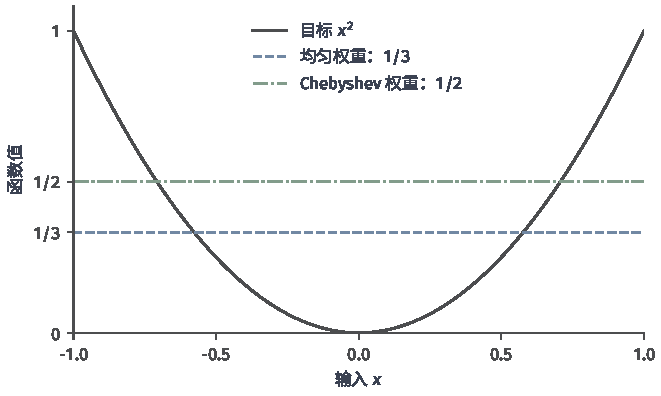
\includegraphics[width=112.0mm]{figures/01-mathematical-preliminaries-upper/02-linear-algebra-and-geometry/matplotlib/concepts-analysis-functional/weighted-projection.pdf}
 \functionalinlinefigurecaption{fig:functional-weighted-projection}
   {对$x^2$使用同一候选空间$\operatorname{span}\{1,x\}$，均匀权重的最佳常数为$1/3$，Chebyshev权重的最佳常数为$1/2$。目标、区间和候选空间保持相同，只改变误差积分的权重。曲线由解析式生成。}
\end{minipage}
\end{center}

区间或权重改变后，正交系数必须随之重算。把$[a,b]$仿射映射到$[-1,1]$可以迁移
Legendre或Chebyshev基，但Jacobian因子和权重也会改变。Chebyshev多项式还具有适合
一致逼近与插值的极值分布；这不意味着其加权$L^2$投影自动就是一致范数下的最佳逼近。
投影结论始终相对于所选内积成立，误差度量一旦改变，最佳函数也可能改变。

\subsection{有限观测下的函数拟合}
\label{sec:functional-finite-observation-fitting}
\label{sec:functional-class-size-smoothness}


有限观测只限制少数读数，候选函数在观测之外仍可能变化。
例如不限制次数与系数的多项式既能拟合平滑趋势，也能在观测之间快速振荡。
要限制这些未观察到的变化，可以先选定函数范数，再给定半径$B\geq0$，考察范数球
\[
  \mathcal{F}_B
  =
  \{f\in\mathcal{V}:\lVert f\rVert_{\mathcal{V}}\leq B\}.
\]
半径限制只有结合范数含义才有信息。$L^2$范数限制函数整体能量，却不直接限制导数；
前面定义的正整数阶Sobolev范数同时限制函数值与相应阶数以内的弱导数，
因而限制导数的平方积分；零阶范数则仍只控制$L^2$能量。Lipschitz约束
$|f(x)-f(z)|\leq L|x-z|$则直接限制输入变化造成的输出变化。它们控制的对象不同，
不能由一个较小的参数数量替代。

在RKHS中，式\eqref{eq:functional-rkhs-pointwise-bound}说明核对角有界时，核范数球
统一控制点值。两个输入之间还有
\begin{equation}
  |f(x)-f(z)|
  \leq
  \lVert f\rVert_{\mathcal{H}_K}
  \lVert K_x-K_z\rVert_{\mathcal{H}_K},
  \label{eq:functional-rkhs-modulus-bound}
\end{equation}
而
\[
  \lVert K_x-K_z\rVert_{\mathcal{H}_K}^2
  =
  K(x,x)+K(z,z)-2K(x,z).
\]
因此，核既确定可用方向，也确定输入变化在空间中有多远；半径再限制沿这些方向的幅度。
改变核与改变正则化强度不是同一操作。

特别地，在$\lVert f\rVert_{\mathcal H_K}\leq B$内，
$|f(x)|\leq B\sqrt{K(x,x)}$，并有
$|f(x)-f(z)|\leq B\sqrt{K(x,x)+K(z,z)-2K(x,z)}$。
若核连续，这给出每个函数的连续性；若右端的核距离还不超过$L_K|x-z|$，
才进一步得到$BL_K$的Lipschitz常数。不能从任意正定核直接推出同一种输入规则性。

现在把这些函数限制用于有限观测。设观测数$n$为正整数，给定有界读取$L_1,\ldots,L_n$及目标读数
$y_1,\ldots,y_n$，一个具体目标是
$J(f)=n^{-1}\sum_i(L_if-y_i)^2+\lambda\lVert f\rVert_{\mathcal H}^2$，其中$\lambda>0$。
平方差惩罚读数误差，范数项惩罚观测之外也可能存在的大幅变化。
可以在全空间求解，也可以另加范数球等可行约束$C$。
先确定如何判断一个候选函数最优，再利用有限读取的结构减少未知方向。
下面的一阶判据也适用于随后使用的其他可微凸目标。

无额外约束且$J$在局部极小点$f^\star$处可微时，沿任意$h$的正负扰动都可行，
所以$DJ(f^\star)[h]=0$，即$\nabla_{\mathcal H}J(f^\star)=0$。
这是必要条件；非凸目标的驻点未必最优，例如实数空间中的$J(a)=-a^2$在零点为驻点，却不是局部极小点。
凸目标和凸可行集允许更强的判据。

\begin{theorem}[凸函数优化的一阶判据]
\label{thm:functional-convex-optimality}
设$C\subseteq\mathcal H$非空且凸，$f^\star\in C$，$J$在$f^\star$的开邻域内
Fréchet可微且在$C$上为有限凸函数。则$f^\star$在$C$上全局最优，当且仅当
\begin{equation}
 \langle\nabla_{\mathcal H}J(f^\star),g-f^\star\rangle_{\mathcal H}\geq0
 \qquad(g\in C).
 \label{eq:functional-convex-optimality}
\end{equation}
\end{theorem}
\begin{proof}
若$f^\star$最优，凸性使$f^\star+t(g-f^\star)$在$0<t\leq1$时可行。
目标差非负，除以$t$再令$t\downarrow0$，便得必要性。
反过来，由目标凸性，
\[
 J(g)-J(f^\star)\geq
 \frac{J(f^\star+t(g-f^\star))-J(f^\star)}{t}.
\]
令$t\downarrow0$，右侧趋于$DJ(f^\star)[g-f^\star]$，
再用所给不等式可得$J(g)\geq J(f^\star)$。
\end{proof}
对$J(g)=\frac12\lVert g-f\rVert^2$，这个判据恰是投影定理中的变分不等式。
定理刻画已经给定的可行点是否最优，没有单独保证最优解存在。
若可行集是单位球面等非凸集合，两点连线未必可行，不能照搬上述必要充分判据。

约束$\lVert f\rVert\leq B$与惩罚$\lambda\lVert f\rVert^2$也不应混用。
前者划定可行函数，后者允许整个空间中的函数参与竞争，只是提高大范数函数的代价。
若$\lambda>0$且某个惩罚问题有有限目标值的解$f_\lambda$，则它也是半径$B=\lVert f_\lambda\rVert$
对应约束问题的一个解；否则范数不更大、拟合更好的函数会降低惩罚目标。
反方向要把给定半径对应到某个乘子，需另有凸性、适当可行性等条件。
第~\ref{chap:optimization}章的一阶判优思路可以这样回用，但有限维KKT条件、
闭有界集的紧性和迭代收敛保证不能原样搬来；梯度迭代还要核对空间中的光滑性等条件。


有限观测看不见的方向是否会出现在最优函数中，取决于惩罚怎样评价这些方向。
整个目标仍可能依赖整函数的范数，
所以“有限读取”只描述拟合项，不表示所有函数取相同读数时目标值都相同。


RKHS可能无限维，但许多训练目标只通过有限个点值读取$f$。再生性质使这些读取方向恰好由
有限个核截面表示\scite{scholkopf2001representer}。

\begin{theorem}[有限样本表示定理]
\label{thm:functional-representer-theorem}
设$\mathcal{H}_K$是$\mathcal{X}$上的RKHS，训练输入为
$x_1,\ldots,x_n$，其中$n$为正整数。令
$\Phi:\mathbb{R}^n\to(-\infty,\infty]$为任意函数，
$\Omega:[0,\infty)\to(-\infty,\infty]$单调不减。考虑
\begin{equation}
  \inf_{f\in\mathcal{H}_K}
  \left\{
    \Phi\bigl(f(x_1),\ldots,f(x_n)\bigr)
    +
    \Omega\bigl(\lVert f\rVert_{\mathcal{H}_K}\bigr)
  \right\}.
  \label{eq:functional-representer-objective}
\end{equation}
若该问题存在最优解，则至少有一个最优解具有形式
\begin{equation}
  f^\star
  =
  \sum_{i=1}^{n}a_iK_{x_i}.
  \label{eq:functional-representer-form}
\end{equation}
若该问题的最优值有限且$\Omega$严格递增，则每个最优解都具有式
\eqref{eq:functional-representer-form}的形式。
\end{theorem}

\begin{proof}
记$M=\operatorname{span}\{K_{x_1},\ldots,K_{x_n}\}$。这是有限维子空间，因而闭。
由投影定理，任意$f\in\mathcal{H}_K$都可唯一分解为
\[
  f=f_M+f_{\perp},\qquad f_M\in M,\quad f_{\perp}\perp M.
\]
对每个训练输入$x_i$，再生性质给出
\[
  f(x_i)
  =
  \langle f_M,K_{x_i}\rangle
  +
  \langle f_{\perp},K_{x_i}\rangle
  =
  f_M(x_i).
\]
因此经验项$\Phi$无法区分$f$与$f_M$。另一方面，正交分解给出
\[
  \lVert f\rVert_{\mathcal{H}_K}^2
  =
  \lVert f_M\rVert_{\mathcal{H}_K}^2
  +
  \lVert f_{\perp}\rVert_{\mathcal{H}_K}^2,
\]
故$\lVert f_M\rVert\leq\lVert f\rVert$。当$\Omega$单调不减时，用$f_M$替换$f$
不会增大目标值。若原问题存在最优解，对任一最优解作此替换便得到$M$中的最优解，也就是
式\eqref{eq:functional-representer-form}。

若最优值有限、$\Omega$严格递增且$f_{\perp}\neq0$，则
$\lVert f_M\rVert<\lVert f\rVert$，经验项不变而惩罚项严格减小，与$f$最优矛盾。
这里最优目标值有限保证经验项与惩罚项都是有限值，因而惩罚项的严格下降确实使总目标
严格下降。
所以每个最优解都必须满足$f_{\perp}=0$。
\end{proof}

定理没有证明式\eqref{eq:functional-representer-objective}必定达到下确界。存在性仍要
由目标的下半连续性、强制性、闭性或其他条件另行保证。它也没有保证系数向量
$(a_1,\ldots,a_n)^{\top}$唯一；若Gram矩阵奇异，不同系数可能表示同一个函数。
单调不减惩罚只保证存在一个有限展开最优解；只有当最优值有限且惩罚严格递增时，才能
排除每个最优解中的非零正交余项。若损失还依赖导数、积分或训练点之外的其他有界线性
泛函，表示空间应加入这些泛函的Riesz表示元，不能仍机械地只写训练点核截面。

这一推广可以直接从证明读出。若拟合项为$\Phi(L_1f,\ldots,L_nf)$，
其中$L_i$是$\mathcal H$上的有界线性泛函，令$h_i$为各自的Riesz表示元，
再取$M=\operatorname{span}\{h_i\}$。对$f_\perp\perp M$，
$L_i(f_\perp)=\langle f_\perp,h_i\rangle=0$，其余范数比较完全不变。
一般的积分读取与系数读取因此也有有限表示；导数读取则必须先验证它在所选空间有界。

\subsubsection{基于有限表示的参数求解}
\label{sec:functional-finite-parameter-solvers}

写$f=\sum_{j=1}^n a_jh_j$，令$\bm a=(a_1,\ldots,a_n)^\top$，定义Gram矩阵
$\bm G\in\mathbb R^{n\times n}$，$\bm G_{i,j}=\langle h_j,h_i\rangle_{\mathcal H}$，则
\[
 (L_1f,\ldots,L_nf)^\top=\bm G\bm a,\qquad
 \lVert f\rVert_{\mathcal H}^2=\bm a^\top\bm G\bm a.
\]
有限表示定理将原问题的下确界化为
\begin{equation}
 \inf_{\bm a\in\mathbb R^n}
 \left\{\Phi(\bm G\bm a)
       +\Omega\!\left(\sqrt{\bm a^\top\bm G\bm a}\right)\right\}.
 \label{eq:functional-finite-gram-objective}
\end{equation}
点值读取时$h_i=K_{x_i}$、$\bm G_{i,j}=K(x_i,x_j)$，即通常的核矩阵。
一般读取则仍用相应表示元的Gram矩阵，而不是把所有观测都改称点值。
有限化之后可以按目标的光滑性、凸性和约束回用第~\ref{chap:optimization}章的方法；
表示定理本身没有指定某个数值算法。

图~\ref{fig:representer-finite-readings-to-solver}串起从有限读取到系数求解的步骤：先删去读数看不见的正交分量，再把读取与范数写成同一个Gram矩阵上的有限表达式。

\begin{figure*}[htbp]
  \centering
  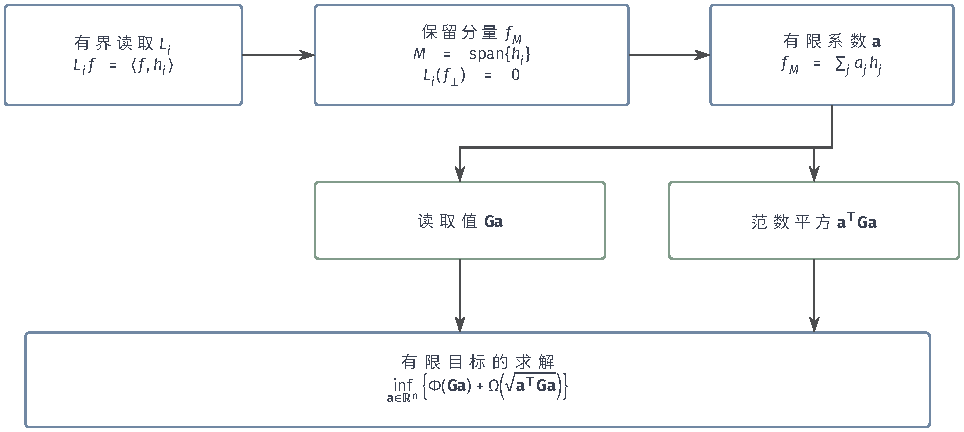
\includegraphics[width=163.258mm]{figures/01-mathematical-preliminaries-upper/02-linear-algebra-and-geometry/tikz/representer-finite-readings-to-solver/source.pdf}
  \caption{有限读取下的表示与求解。有界线性泛函$L_i$在Hilbert空间中有Riesz表示元$h_i$。
  所有读取只依赖$M=\operatorname{span}\{h_i\}$中的分量$f_M$，
  单调不减的范数惩罚允许删去$f_\perp$而不增大目标。
  写$f_M=\sum_j a_jh_j$后，读数与范数平方分别为$\bm G\bm a$与$\bm a^\top\bm G\bm a$。
  将这两个有限表达式代入目标后即可求解系数；最优解存在与系数唯一仍需另行判断。}
  \label{fig:representer-finite-readings-to-solver}
\end{figure*}


平方损失给出可直接核对的实例：
\[
 J(f)=\frac1n\sum_{i=1}^n(L_if-y_i)^2+\lambda\lVert f\rVert_{\mathcal H}^2,
 \qquad\lambda>0.
\]
其中$y_i$是第$i$个读取的目标值，$\bm y=(y_1,\ldots,y_n)^\top$。
将读数和范数代入后，系数目标为
$n^{-1}\lVert\bm G\bm a-\bm y\rVert_2^2+\lambda\bm a^\top\bm G\bm a$，
对$\bm a$求导并约去因子$2/n$，驻点条件为
$\bm G((\bm G+n\lambda\bm I_n)\bm a-\bm y)=0$。
由于$\bm G$半正定，$\bm G+n\lambda\bm I_n$正定，故可先解
\[
 (\bm G+n\lambda\bm I_n)\bm a=\bm y
\]
得到一个驻点。系数目标的Hessian为
$2\bm G^2/n+2\lambda\bm G$，由$\bm G$半正定可知它也半正定，
因此系数目标凸，这个驻点就是全局最优系数。
目标在$f$上严格凸，因而函数解唯一；但若$\bm G$奇异，
给$\bm a$加任意$\bm v\in\ker\bm G$不会改变函数，因为
$\lVert\sum_i v_i h_i\rVert^2=\bm v^\top\bm G\bm v=0$。
所以这个可逆的移位方程只选出了一个系数代表，并未使原系数目标的全部最优系数唯一。
若$h_i$线性无关，Gram矩阵正定，表示系数才唯一。

这也与函数微分吻合。把$L_i h=\langle h,h_i\rangle$代入目标的一阶变化，可得
\[
 \nabla_{\mathcal H}J(f)
 =\frac2n\sum_{i=1}^n(L_if-y_i)h_i+2\lambda f.
\]
梯度为零时，$f$必在读取方向的张成空间内。
这次计算依赖可微平方损失；表示定理的正交分解证明则不要求$\Phi$可微或凸。

\begin{example}[两个点值的有限求解]
\label{ex:functional-two-readings}
在$[-1,1]$的仿射RKHS中，取$x_1=-1,x_2=1$，目标值$y_1=0,y_2=2$，
并令$\lambda=1$。核矩阵为$\bm K=2\bm I_2$，移位方程为
$4\bm a=(0,2)^\top$，得到$\bm a=(0,1/2)^\top$及
$f^\star(x)=(1+x)/2$。也可直接令$f(x)=a+bx$，把目标展开为
\[
 \tfrac12\bigl((a-b)^2+(a+b-2)^2\bigr)+a^2+b^2
 =2(a-1/2)^2+2(b-1/2)^2+1.
\]
所以函数解确为$a=b=1/2$，最优目标值为$1$。
若再使用$x_3=0$，则三个核截面满足
$K_{-1}-2K_0+K_1=0$；函数仍只有两个独立方向，
按输入顺序$(-1,1,0)$排列的三项展开系数因而可以沿$(1,1,-2)^\top$变化而不改变函数。
\end{example}

存在性要在正确的空间里检查。上述平方损失目标连续，且
$J(f)\geq\lambda\lVert f\rVert^2$；在有限维$M$中，最小化序列有界，
可抽出收敛子列并由连续性取得最小值。投影不增加目标，所以这也是全空间最小值。
更一般地，若$J|_M$下半连续、某处有限且强制，即
$\lVert f\rVert\to\infty$时$J(f)\to+\infty$，同样可用有限维紧性。
不必要求冗余系数空间中的目标强制，因其零空间方向可能无界却代表同一个函数。
反例是非零读取$L$对应的$J(f)=e^{-L(f)}$、无范数惩罚：下确界为零，
但没有任何函数达到它。有限表示没有替代存在性。

附加约束$C$时还要检查$P_M(C)\subseteq C$。核范数球满足这一点，
只依赖同一组读数的约束也满足，因为投影不改变读数。
一般约束则未必：在仿射RKHS$f(x)=a+bx$中，只读取$f(0)=a$，
故$M=\operatorname{span}\{1\}$；约束$b=1$却使任何可行函数的投影都不可行。
若目标为$a^2+\lambda(a^2+b^2)$，约束解是$f(x)=x$，确实不在$M$内。
这里可以把系数读取$b=\langle f,x\rangle$的表示方向$x$加入$M$，
再检查投影保留约束。一般导数限制或非凸函数约束不一定有这种有限补充，
不能直接沿用无约束表示公式。

\subsection{整体误差下的函数拟合}
\label{sec:functional-integral-error-fitting}

有限读取只比较若干观测值，整体积分误差则按指定测度评价整条函数。
在Mercer条件下，核的谱坐标可以同时展开平方积分误差与核范数，
从而逐方向求出拟合和惩罚的取舍。这里先给定测度$\mu$；有限训练点不会自动确定它。

\subsubsection{基于谱表示的函数求解}
\label{sec:functional-spectral-fitting-solvers}

给定$y\in L^2(\mu)$，紧自伴谱分解将其写为
\[
 y=y_0+\sum_{j:\mu_j>0}c_j\psi_j,\qquad
 y_0\in\ker T_K,\quad
 \lVert y\rVert_2^2=\lVert y_0\rVert_2^2+\sum_jc_j^2.
\]
RKHS中的函数没有$y_0$方向，故这一分量会留下不可消除的误差。考虑
\[
  \min_{f\in\mathcal{H}_K}
  \left\{
    \lVert f-y\rVert_{L^2(\mu)}^2
    +
    \lambda\lVert f\rVert_{\mathcal{H}_K}^2
  \right\},
  \qquad \lambda>0.
\]
写$f=\sum_jb_j\psi_j$，并要求$\sum_jb_j^2/\mu_j<\infty$，目标成为
\[
 J(f)=\lVert y_0\rVert_2^2+
 \sum_j\left((b_j-c_j)^2+\lambda\frac{b_j^2}{\mu_j}\right).
\]
每个方向的二次式可配方为
\[
 (b_j-c_j)^2+\frac{\lambda}{\mu_j}b_j^2
 =\left(1+\frac{\lambda}{\mu_j}\right)
   \left(b_j-\frac{\mu_j}{\mu_j+\lambda}c_j\right)^2
   +\frac{\lambda}{\mu_j+\lambda}c_j^2.
\]
因而候选最优系数为
\begin{equation}
  b_j^\star
  =
  \frac{\mu_j}{\mu_j+\lambda}c_j.
  \label{eq:functional-spectral-shrinkage}
\end{equation}
还必须确认逐项最优值拼成合法函数。由
$\mu_j/(\mu_j+\lambda)^2\leq1/(4\lambda)$，有
\[
 \sum_j\frac{(b_j^\star)^2}{\mu_j}
 =\sum_j\frac{\mu_j c_j^2}{(\mu_j+\lambda)^2}
 \leq\frac1{4\lambda}\sum_jc_j^2<\infty.
\]
所以$f^\star\in\mathcal H_K$。对有限部分和使用配方，再以非负级数取极限，得到
\[
 J(f)=J(f^\star)+
 \sum_j\left(1+\frac{\lambda}{\mu_j}\right)(b_j-b_j^\star)^2,\qquad
 J(f^\star)=\lVert y_0\rVert_2^2+
 \sum_j\frac{\lambda}{\mu_j+\lambda}c_j^2.
\]
这同时证明存在、最优和唯一，而不只是写出形式驻点。
若$K=0$，核空间只有零函数，空和仍给出$f^\star=0$。
若令$\lambda=0$，核范数可和性不再由上界保证；正谱部分的目标若不属于RKHS，
下确界可能只能由有限截断逼近，不能直接把公式延伸为一个空间内最优解。
特征值远小于$\lambda$的方向被强烈收缩，特征值远大于$\lambda$的方向则大体保留。
这与第\ref{chap:optimization}章的二次正则化是同一逐方向机制；定理
\ref{thm:functional-representer-theorem}的有限表示处理训练点目标，这里的谱解则
处理总体$L^2(\mu)$目标，两者不能省略各自的存在条件而互相替代。

附加约束后，配方仍成立，却未必能逐方向独立取极小值。
例如要求$\lVert f\rVert_{\mathcal H_K}\leq B$会把所有系数通过
$\sum_jb_j^2/\mu_j\leq B^2$耦合；若无约束解超出球，需要重新满足此条件。
点值等式$f(x_0)=a$则成为$\sum_jb_j\psi_j(x_0)=a$，同样联系各个方向。
不能先独立收缩再宣称结果自动满足任意函数约束。

仿射核再次给出有限的核对实例。取$K(x,z)=1+xz$、
$\mathrm d\mu(x)=\mathrm dx/2$和目标$y(x)=x^2$。
其正谱系数为$c_1=1/3,c_2=0$，零空间分量为$y_0=x^2-1/3$，
且$\lVert y_0\rVert_2^2=1/5-1/9=4/45$。因此
\[
 f^\star(x)=\frac{1}{3(1+\lambda)},\qquad
 J(f^\star)=\frac4{45}+\frac{\lambda}{9(1+\lambda)}.
\]
第一项是仿射空间不能表示二次曲线留下的误差，第二项来自正则化对常数方向的收缩。
令$\lambda\downarrow0$时得到均匀权重下的最佳常数$1/3$，
与前面加权投影的直接计算一致。图~\ref{fig:functional-spectral-shrinkage}则展示
有无限多个方向时，同一个收缩因子怎样随方向变化。

\begin{center}
\begin{minipage}{\linewidth}
 \centering
 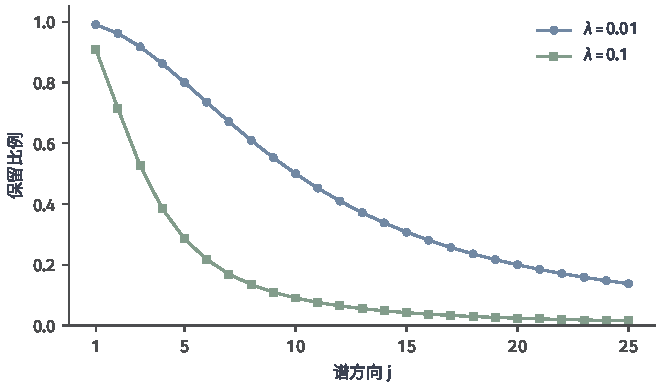
\includegraphics[width=112.0mm]{figures/01-mathematical-preliminaries-upper/02-linear-algebra-and-geometry/matplotlib/analysis-geometry/functional-spectral-shrinkage.pdf}
 \functionalinlinefigurecaption{fig:functional-spectral-shrinkage}
   {教学谱$\mu_j=j^{-2}$上的收缩比例$\mu_j/(\mu_j+\lambda)$。蓝、绿线使用$\lambda=0.01$和$0.1$，点标出前$25$个方向；增大正则化后，各方向的保留比例进一步减小。有效维度的定义仍对全部谱方向求和。}
\end{minipage}
\end{center}

\subsection{平滑能量下的函数与场优化}
\label{sec:functional-smooth-energy-optimization}
\label{sec:geometry-function-field-optimization}
\label{sec:geometry-smoothness-energy-boundary}
\label{sec:geometry-energy-variation-solvers}

现在不再移动一个点，而是在固定流形上调整整个函数$f$或向量场$\bm V$。
例如给点带上的每处位置分配一个标量，既符合观测又避免局部剧烈变化。
切空间中的梯度仍用于测量空间变化，但优化方向本身已是一个函数或向量场。


相同的函数值差，若发生在更短的几何距离内，变化更剧烈。
因此应累计单位长度上的变化，而不是把坐标偏导不加权地平方相加。
\begin{definition}[Dirichlet能量]
\label{def:geometry-dirichlet-energy}
实函数$f$的\term{Dirichlet能量}定义为
\begin{equation}
 \mathcal E(f)=\frac12\int_{\mathcal M}
       \lVert\operatorname{grad}f\rVert_g^2\,\mathrm dV_g.
 \label{eq:geometry-dirichlet-energy}
\end{equation}
对光滑函数按通常导数理解；积分不有限时取$+\infty$。
\end{definition}
度量同时决定梯度和体积。对开带，
$\sqrt{\det\bm G}=1+u/R$且
$\bm G^{-1}=\operatorname{diag}((1+u/R)^{-2},1)$，故
\begin{equation}
 \mathcal E(f)=\frac12\int
 \left[\frac{(\partial_sf)^2}{1+u/R}
       +(1+u/R)(\partial_uf)^2\right]\,\mathrm ds\,\mathrm du.
 \label{eq:geometry-strip-dirichlet-energy}
\end{equation}
外侧相同$\mathrm ds$更长，所以相同$\partial_sf$对应较小的单位长度变化；
与此同时，小坐标盒的实际面积更大。两个权重必须从同一度量共同推导。


在紧域上，不加限制时常量函数已经取得$\mathcal E=0$，
所以“最平滑”不会自动保留观测信号。
可以规定边界值，加入数据拟合积分
$\frac{\lambda}{2}\int|f-y|^2\,\mathrm dV_g$，或施加均值与范数约束。
例如零均值加单位$L^2$范数排除常量，并将问题连到非平凡谱模态。
采用$H^1$候选时，孤立点的函数值在一般维数下未必有良定义的连续评价；
逐点观测约束还要提高正则性或改用局部平均，不能直接当作任意$H^1$函数的属性。

向量场的平滑要先比较不同点的方向，故使用协变导数。
取局部正交归一切基$\bm e_1,\ldots,\bm e_d$，定义
\[
 \lVert\nabla\bm V\rVert_g^2
 =\sum_{a=1}^d\lVert\nabla_{\bm e_a}\bm V\rVert_g^2,\qquad
 \mathcal E_\nabla(\bm V)
 =\frac12\int_{\mathcal M}\lVert\nabla\bm V\rVert_g^2\,\mathrm dV_g.
\]
正交换基不改变这个平方和，所以定义与局部基选择无关。
有限能量空间可相应要求$\bm V$及$\nabla\bm V$平方可积，
边界迹、观测或归一化限制也应针对向量场重新规定。
坐标分量恒定的场未必平行，环境恒定向量也未必处处切向；
向量场不能用“不变的逐坐标数值”代替零协变变化。


取允许扰动$h$，令$f_\epsilon=f+\epsilon h$。
梯度对函数线性，对平方范数求导得到
\begin{equation}
 \left.\frac{\mathrm d}{\mathrm d\epsilon}
  \mathcal E(f+\epsilon h)\right|_{\epsilon=0}
 =\int_{\mathcal M}
    g(\operatorname{grad}f,\operatorname{grad}h)\,\mathrm dV_g.
 \label{eq:geometry-dirichlet-first-variation}
\end{equation}
这是对整个函数的一阶变化，而非沿流形上一条点轨迹的变化。
要识别函数空间中的梯度，需要把$h$上的导数移走。


用Green恒等式~\eqref{eq:geometry-green-identity}改写上述变分，就能把内部作用与边界项分开。
无边界时没有边界项。固定$f$的边界迹时，允许的$h$在边界为零，
这给出Dirichlet条件；边界自由时，要使任意边界扰动的一阶变分为零，
就需$\partial_{\bm n}f=0$，这是自然的齐次Neumann条件。
对未加数据项的能量，内部驻点满足$\Delta_gf=0$。
闭带的两条长边和两个端部都需按问题规定条件，不能只处理图上显眼的一条边。

函数空间也有自己的内积。取
$\langle u,h\rangle_{L^2}=\int_{\mathcal M}uh\,\mathrm dV_g$。
把Dirichlet能量视为$L^2$上的泛函时，有限值需要$f\in H^1$；
若固定Dirichlet边值，还需施加相应的迹约束。这不是$L^2$开邻域上的有限值可微泛函：
$L^2$很小的扰动仍可能具有很大的空间导数，甚至不属于$H^1$。
因此，不能直接套用定义~\ref{def:functional-frechet-gradient}中的
Fréchet微分与梯度。这里先沿允许的$H^1$扰动求一阶变分，再判断这个线性读取
能否用一个$L^2$函数表示。
当$f$位于所选算子域、$\Delta_gf\in L^2$且边界项消失时，
上式把一阶变分表示为
$\delta\mathcal E(f)[h]=\langle-\Delta_gf,h\rangle_{L^2}$。
这里将这个表示函数称为能量的$L^2$梯度，即
$\operatorname{grad}_{L^2}\mathcal E(f)=-\Delta_gf$；
将允许函数以外的能量扩为$+\infty$后，也可用相应凸能量的$L^2$次梯度表述这一关系。


向量场能量按相同思路变分，但导数换成协变导数。
对允许的扰动场$\bm W$，
\[
 \delta\mathcal E_\nabla(\bm V)[\bm W]
 =\int_{\mathcal M}\sum_a
     g(\nabla_{\bm e_a}\bm V,\nabla_{\bm e_a}\bm W)\,\mathrm dV_g.
\]
对每个求导方向作度量相容的分部积分，得到
\begin{equation}
 \delta\mathcal E_\nabla(\bm V)[\bm W]
 =\int_{\mathcal M}g(\nabla^*\nabla\bm V,\bm W)\,\mathrm dV_g
  +\int_{\partial\mathcal M}g(\nabla_{\bm n}\bm V,\bm W)\,\mathrm dS_g,
 \label{eq:geometry-connection-laplacian-variation}
\end{equation}


固定向量场边界迹时$\bm W=0$；自由边界给出自然条件$\nabla_{\bm n}\bm V=0$。
边界项消失后，
$\langle\bm V,\nabla^*\nabla\bm V\rangle_{L^2}
=\int\lVert\nabla\bm V\rVert_g^2\,\mathrm dV_g\geq0$。

\subsubsection{基于梯度流的演化求解}
\label{sec:functional-gradient-flow-solvers}

负梯度流为热方程
\begin{equation}
 \frac{\partial f}{\partial t}=\Delta_gf.
 \label{eq:geometry-heat-equation}
\end{equation}
对足够光滑且满足相应时间不变边界条件的解，
\[
 \frac{\mathrm d}{\mathrm dt}\mathcal E(f_t)
 =-\int_{\mathcal M}(\Delta_gf_t)^2\,\mathrm dV_g\leq0.
\]
热流降低的是整个函数的能量；$\operatorname{grad}f$是每点的切向量，
$\operatorname{grad}_{L^2}\mathcal E$却是一个标量函数，二者不可混称。
换用带权$L^2$或$H^1$内积，表示同一能量微分的梯度会改变，
不能仍无条件使用相同热方程。这里$t$是扩散时间，不是点带的空间坐标$s$。


\begin{example}[圆上的坐标、能量与谱尺度]
\label{ex:geometry-circle-energy-scale}
半径为$R$的完整圆采用角坐标$\theta$，
$g_{\theta\theta}=R^2$、$\mathrm dV_g=R\,\mathrm d\theta$。
取$f(\theta)=\cos\theta$，则
\[
 \begin{aligned}
 \lVert\operatorname{grad}f\rVert_g^2&=\frac{\sin^2\theta}{R^2},\\
 \Delta_gf&=\frac1{R^2}f''=-\frac{\cos\theta}{R^2},\\
 \mathcal E(f)&=\frac12\int_0^{2\pi}
        \frac{\sin^2\theta}{R^2}R\,\mathrm d\theta=\frac{\pi}{2R}.
 \end{aligned}
\]
同一幅度变化放在更大的圆上，单位长度上的变化更小；
该模态的特征值为$1/R^2$，热流幅度按$\exp(-t/R^2)$衰减。
改用局部弧长坐标$s=R\theta$时，度量分量变为$1$，
$f(s)=\cos(s/R)$的导数补入$1/R$，结果不变。
能量使用$1/2$归一化，省去它时能量及其梯度都要同步加倍。
\end{example}


向量场梯度流为$\partial_t\bm V=-\nabla^*\nabla\bm V$。
它的零能量场必须处处平行，未必存在非零者；
标量常量零模的结论不能直接移过来，更不能逐坐标照抄标量Laplace--Beltrami公式。


圆上初值$f_0(\theta)=\cos\theta$的直接解为
$f_t(\theta)=e^{-t/R^2}\cos\theta$，代入热方程即可核对，
其能量为$e^{-2t/R^2}\pi/(2R)$。这一模态趋于零，
一般初值中的常量模态则保留；能量下降本身并不证明任意演化或离散算法都收敛。

\section{收敛与逼近}
\label{sec:functional-convergence-approximation}

同一个函数可以由求解迭代或展开截断逐步得到，两种序列的生成规则不同。
改变表示规模、采样或惩罚尺度，又会改变可达到的逼近误差。
本节先比较函数序列的一般收敛方式，再分别建立这些具体条件下的结论；
最后从单个目标转向整个函数类，研究预先准备多少代表才能满足统一误差要求。

\subsection{函数序列的收敛}
\label{sec:functional-sequence-convergence}

范数收敛要求$\lVert f_n-f\rVert\to0$；逐点收敛要求每个固定$x$的读数收敛，
一致收敛则用同一个误差界控制所有输入。这些量词不能互换。
若一个点的读取有界，范数收敛会推出该点读数收敛；
若读取界对输入统一，还可得到一致控制。没有这些条件，积分范数收敛不控制固定点值。
在$[0,1]$上令
\[
  f_n(x)=\max\{1-nx,0\},
\]
则$\lVert f_n\rVert_{L^2}^2=1/(3n)\to0$，但
$\lVert f_n\rVert_{\infty}=1$始终不变。平方积分可直接计算：
$\int_0^{1/n}(1-nx)^2\,\mathrm dx=1/(3n)$。
图~\ref{fig:functional-point-evaluation}中峰宽缩小而峰高不变，正好区分了这两种误差。

\begin{center}
\begin{minipage}{\linewidth}
 \centering
 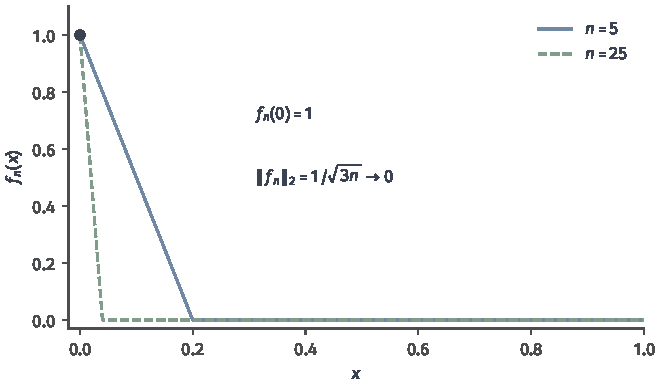
\includegraphics[width=112.0mm]{figures/01-mathematical-preliminaries-upper/02-linear-algebra-and-geometry/matplotlib/analysis-geometry/functional-point-evaluation.pdf}
 \functionalinlinefigurecaption{fig:functional-point-evaluation}
   {连续尖峰$f_n(x)=\max\{1-nx,0\}$在$L^2$范数下趋于零，原点函数值却始终为$1$。峰宽分别为$1/5$和$1/25$；蓝、绿线均由解析式生成。整体能量控制不等于稳定的点值控制。}
\end{minipage}
\end{center}


无限维还使一些有限维中自动成立的性质需要单独检查。有限维子空间仍然总是闭集，
但一般无限维子空间未必闭；有限维中的有界序列有收敛子列、线性映射自动连续，
在一般无限维空间中也可能失效。例如
$\ell^2$中的标准单位向量$(\bm{e}_j)_{j\geq1}$都位于单位球内，但$j\neq k$时
\[
  \lVert\bm{e}_j-\bm{e}_k\rVert_2=\sqrt{2}.
\]
这个序列没有柯西子列，因而也没有收敛子列。无限维闭单位球由此给出“闭且有界未必紧”
的具体反例；这里具体指$\ell^2$的闭单位球。


第\ref{sec:functional-decomposition-projection}节的完备性只在序列已是柯西列时保证空间内极限。
范数变化也可能改变极限是否存在：连续函数以积分误差趋近阶跃函数，
并不说明它们在一致范数下形成柯西列。有限维的任意范数等价与闭有界紧性，
在无限维函数范围内须重新验证。

\subsection{求解和优化下的迭代序列收敛}
\label{sec:functional-iteration-convergence}

有限读取拟合化为有限系数目标后，可回用第~\ref{chap:linear-algebra-and-matrix-analysis}章的线性求解与梯度迭代结论。
若$f^{(k)}=\sum_i a_i^{(k)}h_i$且目标函数解由$a^*$表示，则
\[
 \lVert f^{(k)}-f^*\rVert_{\mathcal H}^2
 =(\bm a^{(k)}-\bm a^*)^\top\bm G(\bm a^{(k)}-\bm a^*).
\]
系数趋近一个最优代表因而使函数误差的范数趋零；有界读取又保证预测趋近。
反方向不一定成立：$\ker\bm G$中的系数变化不改变函数。
若用$\bm G+n\lambda\bm I$的正定方程生成迭代，
其谱与步长条件依第~\ref{chap:linear-algebra-and-matrix-analysis}章判断；若直接迭代原冗余系数目标，
则要区分可见方向的收敛与零方向保留的初始分量。
一般损失还需验证实际目标的光滑、凸性或其他算法假设，
有限表示定理没有额外提供收敛保证。

\subsection{展开截断下的函数序列收敛}
\label{sec:functional-truncation-convergence}

固定完备正交系后，前$m$项的投影是一个明确的序列。
由式~\eqref{eq:functional-projection-error-decomposition}与Parseval等式，
\[
 \lVert f-P_mf\rVert_{\mathcal H}^2
 =\sum_{j>m}|\langle f,e_j\rangle|^2\to0.
\]
它比较同一个目标与嵌套的方向集合；若正交系不完备，
极限只是目标在其闭张成上的投影，仍留下不可表示余项。
每个截断在当前方向集合中最佳，却未必在所有同规模非线性表示中最佳。

Mercer条件下，$f=\sum_j b_j\psi_j$的RKHS截断尾误差为
$\sum_{j>m}b_j^2/\mu_j$，$L^2$尾误差为$\sum_{j>m}b_j^2$。
RKHS范数误差还通过统一有界的核对角控制一致误差；
仅有$L^2$截断收敛不能作同样推断。定义域、范数和所选方向决定每一项误差的含义。

\subsection{有限表示约束下的函数逼近}
\label{sec:functional-approximation-capacity-representation}

固定定义域、目标集合和误差尺度之后，有限表示可以采取全局多项式、局部片段、
非线性单元或可分离因子的形式。下面分别说明怎样构造、误差怎样控制，以及哪些条件
不能由“存在一个表示”推出。

先用同一个目标比较这些有限表示。取
\[
  f_\star(x)=\left|x-\frac12\right|,
  \qquad x\in[0,1],
\]
可以看清表示选择的差异。全局多项式用一组遍及整个区间的基函数逼近折点；分段线性样条
只需把$1/2$设为结点，就能精确表示$f_\star$。使用宽度$\sigma>0$的高斯核
\[
  K_\sigma(x,z)
  =
  \exp\left(-\frac{(x-z)^2}{2\sigma^2}\right)
\]
时，可以由若干主要作用于中心附近的核截面$K_\sigma(\,\cdot\,,x_i)$组合出平滑逼近。
高斯核离开中心后衰减，却没有紧支撑；“局部”不表示中心以外恰好为零。有限组合仍是
光滑函数，不能在有限核宽度下精确产生折点。

令$\operatorname{ReLU}(t)=\max\{t,0\}$。带ReLU激活的单隐藏层网络则可直接写成
\[
  f_\star(x)
  =
  \operatorname{ReLU}\left(x-\frac12\right)
  +
  \operatorname{ReLU}\left(\frac12-x\right).
\]
当$x>1/2$时，第一项为$x-1/2$、第二项为零；当$x<1/2$时，第二项为$1/2-x$、第一项为零。
$x=1/2$时两项都为零。
两个单元恰好接成所需的折线。

多项式、样条、高斯截面和ReLU对折点的表达不同，区别来自各自允许的函数形状。
选择表示时，应核对它与目标规则性的匹配，而不能只比较哪一类更通用。
相比之下，正定核$1+xz$始终只产生仿射函数，不能任意精度逼近折点目标。

\begin{fullwidth}
\begin{minipage}{\linewidth}
 \centering\small
 \begin{tabularx}{\linewidth}{@{}lXX@{}}
 \toprule
 表示 & 对$f_\star(x)=|x-1/2|$的有限表示 & 调整的范围\\
 \midrule
 全局多项式 & 可逼近，有限次数不能精确产生折点 & 一个系数通常影响整个区间\\
 分段线性样条 & 将$1/2$设为结点即可精确表示 & 结点邻域内的分段变化\\
 固定正宽度的高斯核有限和 & 保持光滑，可逼近但不能精确产生折点 & 核中心附近的变化，宽度决定影响范围\\
 两个ReLU单元 & 上式直接给出精确表示 & 隐藏单元的位置和方向决定折点\\
 \bottomrule
 \end{tabularx}
 \functionalinlinetablecaption{tab:functional-representation-comparison}
   {同一个连续目标的不同表示。有限表示的结构与整个表示族的稠密性是不同问题。}
\end{minipage}
\end{fullwidth}


\subsubsection{基于多项式的函数逼近}
\label{sec:functional-polynomial-approximation}

沿用定义~\ref{def:functional-density}的稠密性，下面不再只判断极限是否存在，
而是寻找能随目标与精度构造出的具体表示。稠密性是一项表示存在性结论：它允许逼近器依赖目标和精度，却
没有说明需要多少参数、怎样找到逼近器，或从有限观测能否识别它。

多项式提供一个基本例子。对$f\in C([0,1])$及正整数$m$，定义Bernstein多项式
\begin{equation}
  (B_mf)(x)
  =
  \sum_{j=0}^{m}
  f\left(\frac{j}{m}\right)
\binom{m}{j}x^j(1-x)^{m-j}.
  \label{eq:functional-bernstein-polynomial}
\end{equation}
权重非负且由二项式定理知其和为$1$，所以$B_mf(x)$是网格函数值的加权平均。
这里的“平均”只是有限非负权重之和；下面只用第~\ref{chap:combinatorics}章的
二项式恒等式和第~\ref{chap:mathematical-analysis}章的一致连续性，不预先调用概率论。

\begin{theorem}[Bernstein逼近定理]
\label{thm:functional-weierstrass-bernstein}
对每个$f\in C([0,1])$，
\[
  \lVert B_mf-f\rVert_{\infty}\longrightarrow0.
\]
因此，多项式在$C([0,1])$的一致范数下稠密。
\end{theorem}

\begin{proof}
连续函数在紧区间上一致连续且有界。记
$M=\lVert f\rVert_{\infty}$。给定$\varepsilon>0$，可取$\delta>0$使
$|u-x|<\delta$时$|f(u)-f(x)|<\varepsilon/2$。

对固定$x$，把式\eqref{eq:functional-bernstein-polynomial}中的权重记为
$w_{m,j}(x)$。由$j\binom mj=m\binom{m-1}{j-1}$和
$j(j-1)\binom mj=m(m-1)\binom{m-2}{j-2}$，有
$\sum_jj w_{m,j}=mx$及$\sum_jj(j-1)w_{m,j}=m(m-1)x^2$。
这些组合关系分别对$j\geq1$和$j\geq2$使用；$m=1$时第二个求和直接为零。
将$j^2=j(j-1)+j$代入并展开平方，便得
\[
  \sum_{j=0}^{m}
  \left(\frac{j}{m}-x\right)^2w_{m,j}(x)
  =
  \frac{x(1-x)}{m}
  \leq\frac{1}{4m}.
\]
将网格点分为
$|j/m-x|<\delta$与$|j/m-x|\geq\delta$两组。近处一组的函数值差小于
$\varepsilon/2$。远处一组的总权重满足
\[
  \sum_{|j/m-x|\geq\delta}w_{m,j}(x)
  \leq
  \frac{1}{\delta^2}
  \sum_{j=0}^{m}
  \left(\frac{j}{m}-x\right)^2w_{m,j}(x)
  \leq\frac{1}{4m\delta^2}.
\]
因此对所有$x\in[0,1]$，
\[
  |B_mf(x)-f(x)|
  \leq
  \frac{\varepsilon}{2}
  +
  2M\frac{1}{4m\delta^2}.
\]
取$m$足够大使第二项不超过$\varepsilon/2$，便得到一致误差不超过
$\varepsilon$。界对所有$x$使用同一个$m$，所以结论是一致收敛。
\end{proof}

证明展示了规则性怎样影响逼近：目标的一致连续性控制近处网格值的变化，二项式权重的二阶
离散矩控制远处权重。如果已知更强的光滑性，可以得到更具体的误差速率；只有连续性时，
定理仍给出存在性，但不承诺对所有连续函数共享一个与目标无关的快速速率。

这个构造还可以验证第\ref{sec:functional-scalar-readouts}节高斯核截面族的逼近能力。
固定宽度的核截面族可以一致逼近$[0,1]$上的连续函数，这还需超出正定性的理由。
记$w(x)=e^{-x^2/(2\sigma^2)}$。对中心$z$求导并在$z=0$取值，前三项为
\[
 K_\sigma(x,0)=w(x),\quad
 \partial_zK_\sigma(x,0)=w(x)\frac{x}{\sigma^2},\quad
 \partial_z^2K_\sigma(x,0)=w(x)\left(\frac{x^2}{\sigma^4}-\frac1{\sigma^2}\right).
\]
一般第$k$阶导数为$w(x)p_k(x)$，其中$p_k$的次数为$k$、最高次系数为$\sigma^{-2k}$。
这可由$K_\sigma(x,z)=w(x)e^{xz/\sigma^2}e^{-z^2/(2\sigma^2)}$逐次求导看出：
全部导数落在第一个含$z$的指数上时产生最高次项，其余项的次数更低。
因此先用$p_0$表示常数，再逐次消去最高次项，$p_0,\ldots,p_k$就能张成所有至多$k$次多项式。

这些导数也属于核截面有限线性组合的一致闭包。固定$k\geq1$后，取$h>0$且$kh\leq1$，
差分
\[
 h^{-k}\sum_{j=0}^k(-1)^{k-j}\binom kj K_\sigma(x,jh)
\]
只使用域内中心$0,h,\ldots,kh$。反复使用微积分基本定理，这个差分等于
$\partial_z^kK_\sigma(x,\cdot)$在$z=h(t_1+\cdots+t_k)$、$t_i\in[0,1]$上的平均。
该导数在紧矩形上连续，故这个平均随$h\downarrow0$一致于$x\in[0,1]$地趋于
$\partial_z^kK_\sigma(x,0)$。于是核截面张成的闭包包含每个$w(x)p(x)$。
最后，对连续函数$f/w$使用Bernstein逼近；由于$0<w\leq1$，
$\lVert wp-f\rVert_\infty\leq\lVert p-f/w\rVert_\infty$，所需误差也能任意小。
这里中心数可以增长；有限个固定中心本身不构成稠密族。

\subsubsection{基于样条的函数逼近}
\label{sec:functional-spline-approximation}

多项式同时调整全域系数，分段线性样条则把改动限制在少数相邻区间。
样条是在每段使用低次多项式、并在结点满足指定衔接条件的函数；这里使用连续的分段直线。
设
$a=x_0<x_1<\cdots<x_m=b$，最大网格宽度为
$h=\max_{0\leq j<m}(x_{j+1}-x_j)$。令$S_hf$在结点处等于$f$，
在每个小区间上线性插值，即对$x\in[x_j,x_{j+1}]$定义
\[
 (S_hf)(x)=
 \frac{x_{j+1}-x}{x_{j+1}-x_j}f(x_j)
 +\frac{x-x_j}{x_{j+1}-x_j}f(x_{j+1}).
\]
两个系数非负且和为一，这就是由端点值计算区间内近似值的具体规则。

若$\omega_f(h)=\sup_{|x-z|\leq h}|f(x)-f(z)|$是$f$的连续模，则
\[
  \lVert f-S_hf\rVert_\infty\leq\omega_f(h).
\]
这是因为区间内的插值值是两个端点函数值的凸组合，每个端点距当前点都不超过$h$。

当$f$二阶连续可微时，插值余项进一步给出
\[
  \lVert f-S_hf\rVert_\infty
  \leq
  \frac{h^2}{8}\lVert f''\rVert_\infty.
\]
常数$1/8$来自每段的几何关系。固定区间内部一点$x$，令$e=f-S_hf$，
选择$c$使$q(t)=e(t)-c(t-x_j)(t-x_{j+1})$在$x$处也为零。
$q$在两个端点及$x$处有三个零点，两次Rolle定理给出某个$\xi$满足
$q''(\xi)=f''(\xi)-2c=0$。因此
$e(x)=f''(\xi)(x-x_j)(x-x_{j+1})/2$。
两距离的乘积至多为$(x_{j+1}-x_j)^2/4$，便得到上述上界；
端点的插值误差本来就是零。
前一个界只依赖连续性，后一个界用更强规则性换取二阶误差。

误差以外，单个系数的影响范围也值得比较。在固定结点位置时，改变一个样条结点的函数值只改变相邻
片段，而改变一个全局多项式系数通常会影响整个区间；这是局部表示与全局表示的结构差别，
不是两种误差范数之间的优劣结论。
为看清“一个局部改动”的范围，图~\ref{fig:functional-basis-locality}固定同一个中心，
只增加一个单位系数。样条帽函数在相邻结点外严格为零；Bernstein基在整个开区间内非零；
高斯基$\phi_c(x)=\exp(-(x-c)^2/(2\sigma^2))$虽快速衰减，仍在所有位置非零。
此处它只是显式给定的普通基函数，不需要再生核理论。
局部性需要由基函数的支撑或衰减式判断，不能由参数个数判断。
\begin{center}
\begin{minipage}{\linewidth}
 \centering
 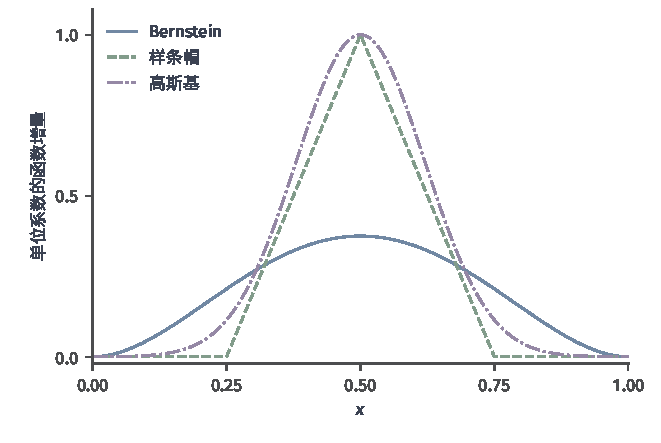
\includegraphics[width=112.0mm]{figures/01-mathematical-preliminaries-upper/02-linear-algebra-and-geometry/matplotlib/teaching-analysis/functional-basis-locality.pdf}
 \functionalinlinefigurecaption{fig:functional-basis-locality}
   {单个系数改变对函数的影响。蓝线为$6x^2(1-x)^2$，即四阶Bernstein多项式的中心基；绿线为中心$1/2$、相邻结点$1/4,3/4$的线性样条帽；紫线为中心$1/2$、宽度$0.12$的高斯基。系数增量均为$1$，不另行缩放峰高；图比较作用范围，未比较三种方法的最优逼近误差。}
\end{minipage}
\end{center}

例如$f(x)=x^2$在$[0,1]$只取结点$0,1$时，插值为$x$，最大误差
$\max_x(x-x^2)=1/4$，恰好等于$h^2\lVert f''\rVert_\infty/8$。
再加入结点$1/2$，最大网格宽度减半，最大误差成为$1/16$。
这里目标固定、网格加密，二阶误差界明确说明了精度怎样随网格变化。

\subsubsection{基于神经网络的函数逼近}
\label{sec:functional-neural-approximation}

前面的折点目标$f_\star(x)=|x-1/2|$已用两个ReLU单元精确表示。
再次写出这个表示，是为了检查每个单元的输入权重与偏置怎样确定折点：
\[
 f_\star(x)=\operatorname{ReLU}(x-1/2)+\operatorname{ReLU}(1/2-x).
\]
两个单元的偏置将折点放在$1/2$，输入系数的正负决定折点哪一侧激活。
更一般的单隐藏层网络把有限个$\sigma(\bm w_j^\top\bm x+b_j)$相加，
$\sigma$称为激活函数，$b_j$为偏置，单元数$m$称为宽度。
网络表示的逼近能力也需要写清激活条件。仅仅“含非线性”还不够：若
$\sigma(t)=t^2$，所有单隐层有限和仍是次数至多为$2$的多项式，无论增加多少单元都不能
得到任意高次目标。下面的结论允许增加宽度，并要求隐藏单元具有偏置。

\begin{theorem}[单隐藏层的通用逼近]
\label{thm:functional-universal-approximation}
设$\mathcal X\subseteq\mathbb R^d$为非空紧集，$f:\mathcal X\to\mathbb R$连续，
$\sigma:\mathbb R\to\mathbb R$连续且不是多项式。对任意$\varepsilon>0$，存在有限
宽度$m$、实数$a_j,b_j,c$以及$\bm w_j\in\mathbb R^d$，使
\begin{equation}
 \begin{aligned}
 g(\bm x)&=c+\sum_{j=1}^m a_j\sigma(\bm w_j^{\top}\bm x+b_j),\\
 \sup_{\bm x\in\mathcal X}|g(\bm x)-f(\bm x)|&<\varepsilon.
 \end{aligned}
 \label{eq:functional-universal-approximation}
\end{equation}
\end{theorem}

这是Leshno等结果在连续激活情形下的表述\scite{leshno1993approximation}。
Sigmoid、Tanh与ReLU都满足激活条件；定理不要求处处可微。连续S形激活在两端分别趋于
$0$与$1$，是非多项式条件的一个常见特例。特别地，紧立方体上的有限和
\begin{equation}
 g(\bm x)=\sum_{j=1}^m a_j\sigma(\bm w_j^{\top}\bm x+b_j)
 \label{eq:functional-sigmoidal-network}
\end{equation}
已能一致逼近连续目标。定理证明涉及更一般的函数空间分离与激活的非多项式性质；本章
前面的Bernstein证明提供稠密性的完整构造，折线与ReLU的对应则给出一维网络版本的直接
构造直觉。

宽度$m$是在给定$f$和$\varepsilon$之后选择的。存在某个表示不保证固定宽度足够，
也不保证训练算法找到参数、有限样本足够或紧集之外的外推准确。向量值目标可以逐坐标
使用结论，再合并有限个单元；目标含跳跃时则不能套用连续目标的一致逼近结论。

不同激活与误差空间还有其他普适逼近版本，但每个版本都必须重新写清定义域、目标集合和
激活条件。它们共同的量词形式是
\[
  \forall f\ \forall\varepsilon>0\
  \exists\text{网络规模与参数，使误差小于 }\varepsilon.
\]
这个陈述没有给出以下任何一项无条件保证：所需网络很小，参数能由可承受的计算找到，
训练算法会到达该参数，或者有限样本上的拟合会在新输入上保持准确。多项式的稠密性也有
同样边界。表示存在、参数规模、优化可计算性和统计泛化是四个不同问题。

误差范数同样决定结论。若只要求$L^2$误差小，逼近器可以在小测度区域出现较大尖峰；若
要求一致误差小，则必须同时控制所有输入。若目标定义在非紧域上，还需要指定加权范数、
局部一致收敛或尾部条件。若目标含不连续点，连续逼近器不可能在整个定义域上一致收敛到
目标，却仍可能在$L^p$意义下逼近。讨论“普适”时必须同时写清目标集合、定义域、逼近器
的并集和误差度量。

\subsubsection{基于分离表示的函数逼近}
\label{sec:functional-separated-approximation}

前面的基函数、局部片段与非线性单元都描述同一个目标函数。
若目标的自变量能够分成两组，还可以把每项写成两组变量各自函数的乘积，
以少量乘积项压缩二者的联合作用。这就是函数的分离表示与低秩结构。
这里沿用第~\ref{chap:linear-algebra}章已经建立的矩阵秩与因子分解。
设$p\in\mathcal{P}$表示一种预测或模型索引，
$q\in\mathcal{Q}$表示一种查询、条件或检验索引，量
$E(p,q)\in\mathbb{R}$记录二者组合后的函数值或误差。选取有限对象
$p_1,\ldots,p_m$与$q_1,\ldots,q_n$，可组成矩阵
\[
  \bm{E}_{i,j}=E(p_i,q_j).
\]
若存在映射$\bm{u}:\mathcal{P}\to\mathbb{R}^r$与
$\bm{v}:\mathcal{Q}\to\mathbb{R}^r$使
\begin{equation}
  E(p,q)
  =
  \langle\bm{u}(p),\bm{v}(q)\rangle,
  \label{eq:functional-bilinear-factorization}
\end{equation}
则任意有限矩阵$\bm{E}$的秩至多为$r$。低秩的含义是所有双索引变化都可由$r$个潜在
方向组合，而不是矩阵元素数目少。

Cauchy--Schwarz不等式还把因子尺度传到每个矩阵元素：
\[
  |E(p,q)|
  \leq
  \lVert\bm{u}(p)\rVert_2
  \lVert\bm{v}(q)\rVert_2.
\]
所以秩控制可用方向数，因子范数控制沿这些方向能够产生的幅度。
分离秩至多$r$的函数集合通常不凸：两个各含$r$个乘积方向的表示相加，
可能需要$2r$个独立方向。因此，将秩上限作为拟合约束时，不能直接套用凸可行集的一阶判据。

秩本身只计方向数，不控制数值尺度。若把因子同时变换为
$\bm{u}'(p)=c\bm{u}(p)$和
$\bm{v}'(q)=\bm{v}(q)/c$，其中$c\neq0$，则式
\eqref{eq:functional-bilinear-factorization}不变，单边因子范数却可以任意改变。
因此，用低秩结构控制误差或计算时，通常还要固定
\[
  \sup_{p\in\mathcal{P}}\lVert\bm{u}(p)\rVert_2\leq B_u,
  \qquad
  \sup_{q\in\mathcal{Q}}\lVert\bm{v}(q)\rVert_2\leq B_v,
\]
或采用对这种缩放更稳定的矩阵范数。方向数$r$与幅度$B_uB_v$承担不同作用。

严格低秩也可能过强。若存在
\[
  E(p,q)
  =
  \langle\bm{u}(p),\bm{v}(q)\rangle+\eta(p,q),
  \qquad
  \sup_{p,q}|\eta(p,q)|\leq\delta,
\]
则$r$描述结构化主项的方向数，$\delta$描述剩余表示误差。增大$r$可能减小$\delta$，
但不会自动给出怎样找到因子、怎样选择查询或怎样由有限观测估计矩阵。代数上的低秩、
因子范数、逼近误差、数据访问条件和计算过程仍须分别说明。

例如在$[-1,1]^2$上取$E(p,q)=\exp(pq)$，用Taylor有限和得到
\[
 E_r(p,q)=\sum_{k=0}^{r-1}\frac{p^kq^k}{k!}
 =\langle\bm u(p),\bm v(q)\rangle,\qquad
 u_{k+1}(p)=\frac{p^k}{\sqrt{k!}},\quad
 v_{k+1}(q)=\frac{q^k}{\sqrt{k!}}.
\]
因为$|pq|\leq1$，余项满足
$\sup_{p,q}|E-E_r|\leq e/r!$，且两侧因子范数平方都不超过
$\sum_{k=0}^{r-1}1/k!\leq e$。这里方向数、因子尺度和一致余项分别得到了控制；
并未声称$r$项是最佳低秩逼近，也没有从不完整观测中恢复因子。

强化学习中的某些复杂度概念会把模型与分布之间的Bellman残差组织成类似矩阵，再研究其
秩或因子化结构。那里的矩阵条目、可实现性、查询协议和样本保证依赖具体决策对象，必须在
相应章节重新定义。仅仅看到某个双线性表达，既不能直接称其为Bellman秩，也不能推出高效
学习。本节提供的是识别这类结构时所需的共同语言。

\subsection{有限采样下的能量逼近}
\label{sec:functional-sampled-energy-approximation}
\label{sec:geometry-sampled-geometric-operators}

只有点云时，常以近邻函数值差构造离散平滑代价
\[
 \mathcal E_n(\bm f)=\frac12\sum_{i,j}w_{i,j}(f_i-f_j)^2.
\]
这里约定求和遍历有序点对，取对称非负边权；同一无向边出现两次，
其他文献的$1/2$或$1/4$系数需连同边权归一化一起比较。
这个形式如何由图拉普拉斯得到，留给
第~\ref{part:discrete-mathematics-and-graph-theory}部分。
本节关注的是它究竟近似哪个连续能量。

先取正整数$n$，在$[0,1]$上取规则网格$x_i=ih$，$i=0,\ldots,n$，$h=1/n$，并固定$f\in C^1([0,1])$。
令$f_i=f(x_i)$，只连接相邻点，取$w_{i,i+1}=w_{i+1,i}=1/(2h)$，其余边权为零。
代入有序点对求和的约定，得到
\[
 \mathcal E_n(\bm f)=\frac12\sum_{i=0}^{n-1}h
 \left(\frac{f(x_{i+1})-f(x_i)}h\right)^2
 \longrightarrow\frac12\int_0^1|f'(x)|^2\,\mathrm dx.
\]
中值定理把第$i$个差商写为某个$\xi_i\in(x_i,x_{i+1})$处的$f'(\xi_i)$，
因此左式是连续函数$|f'|^2/2$的Riemann和，收敛结论随之成立。
这里边权中的$1/h$同时补偿差值里的长度因子与积分单元宽度。
若还要用离散内积逼近$L^2$内积，可给内部节点质量$h$、两端节点各$h/2$，
得到梯形求积。这个例子只证明固定光滑函数的能量值收敛，
没有把它扩大成离散最优解或梯度流收敛；不规则点云还需处理下面的采样差异。

若样本独立同分布于概率测度$q\,\mathrm dV_g$，且$\int|f|q\,\mathrm dV_g<\infty$，
样本平均在大数律条件下趋于$\int f q\,\mathrm dV_g$，而非几何体积积分。
双重样本求和还可能带入两个采样密度因子；邻域核宽、维数相关的尺度系数、
密度估计和权重归一化共同决定极限，不能只看二次型的外观。
例如目标若明确改为
$\mathcal E_q(f)=\frac12\int q\lVert\operatorname{grad}f\rVert_g^2\,\mathrm dV_g$，
在$q>0$光滑且边界项消失时，分部积分给出
\[
 \delta\mathcal E_q(f)[h]
 =-\int h\,\operatorname{div}_g(q\operatorname{grad}f)\,\mathrm dV_g.
\]
相对于$L^2(q\,\mathrm dV_g)$内积，这给出的形式负梯度为
$q^{-1}\operatorname{div}_g(q\operatorname{grad}f)$，一般不等于$\Delta_gf$。
要把它称为该Hilbert空间中的负梯度，还要求$f$满足所选边界条件，
且这个表达式属于$L^2(q\,\mathrm dV_g)$；其定义域可按前面的能量弱形式规定。
若仍采用$L^2(\mathrm dV_g)$内积，形式负梯度则为
$\operatorname{div}_g(q\operatorname{grad}f)$，同样要检验相应的平方可积性。
能量权重与求梯度的内积都要明确。

离散时，代表局部体积的质量权重也影响函数空间内积，
从而影响由同一离散能量得到的演化算子。
边权非负、矩阵对称只能证明某个离散二次型非负，
不能证明它逼近指定的Laplace--Beltrami算子。
至少还要核对流形正则性、采样覆盖与密度、邻域随样本量缩小的速率、
噪声相对尺度的大小，以及边界附近邻域被截断后的处理。
固定边界值与无通量条件并不由同一套未加说明的边规则自动实现。

向量场离散还要给出跨点比较。设$\bm V_i\in T_{\bm p_i}\mathcal M$，
对每条邻边选定$P_{i\leftarrow j}:T_{\bm p_j}\mathcal M\to T_{\bm p_i}\mathcal M$，
才可形成
\[
 \mathcal E_{n,\nabla}(\bm V)
 =\frac12\sum_{i,j}w_{i,j}
      \lVert\bm V_i-P_{i\leftarrow j}\bm V_j\rVert_{g_{\bm p_i}}^2.
\]
若取短测地路径的平行移动，需确保相应路径已选定；
处在凸正规邻域内时有唯一的局部选择。
若只估计了切平面，可用局部对齐近似，但须分析方向估计及搬运误差。
等距搬运且反向为逆映射时，两端的比较一致；
普通环境投影未必具备这些性质。
非负离散能量同样不自动保证连续联络拉普拉斯的一致近似。

\subsection{惩罚尺度变化下的函数逼近}
\label{sec:functional-penalty-scale-approximation}

固定目标$y\in L^2(\mu)$与核，考察第\ref{sec:functional-spectral-fitting-solvers}节
得到的函数解$f_\lambda$怎样随惩罚尺度变化。写
$y=y_0+y_+$，其中$y_0\in\ker T_K$、
$y_+=\sum_jc_j\psi_j$，则
\[
 \lVert f_\lambda-y\rVert_{L^2}^2
 =\lVert y_0\rVert_{L^2}^2+
   \sum_j\left(\frac{\lambda}{\mu_j+\lambda}\right)^2c_j^2.
\]
当$\lambda\downarrow0$时，每项正谱误差趋零且不超过$c_j^2$。
先控制可求和尾项，再控制有限个前项，便得$f_\lambda\to y_+$于$L^2$。
只有$y_0=0$时才逼近整个目标，零空间误差不会因减小惩罚消失。
若$y_+\in\mathcal H_K$，同样用可求和的$c_j^2/\mu_j$控制尾项，
得到RKHS范数收敛；若$\sum_jc_j^2/\mu_j=\infty$，
则$\lVert f_\lambda\rVert_{\mathcal H_K}\to\infty$：任意有限部分和都趋于对应的
$\sum_{j\leq m}c_j^2/\mu_j$，而这些和没有统一上界。
所以$L^2$逼近不保证目标或极限仍属于RKHS。
当$\lambda\to\infty$时，收缩系数趋零，$f_\lambda\to0$于$L^2$。
这些结论比较的是已经求出的最优函数族，不是某个数值算法的迭代序列。

矩阵迹汇总有限个方向的贡献；无限维空间中的方向可能有无穷多个，因此还要核对这份
总量是否有限。下面把算子条件与所选正则化尺度分开。
\begin{definition}[迹类条件与有效维度]
\label{def:functional-trace-effective-dimension}
设$A$为Hilbert空间上的紧线性算子。$A^*A$的正特征值开方后得到奇异值$s_j(A)$，
按重数排列；若只有有限个，可在其后补零。若$\sum_j s_j(A)<\infty$，称$A$为
\term{迹类算子}（trace-class operator）。对正算子，这等价于非负特征值之和有限，
它的迹就是这个和。

若紧正算子$T_K$的正特征值为$(\mu_j)$，给定$\lambda>0$，其
\term{有效维度}（effective dimension）定义为
\begin{equation}
  d_{\mathrm{eff}}(\lambda)
  =
  \sum_{j:\mu_j>0}\frac{\mu_j}{\mu_j+\lambda},
  \label{eq:functional-effective-dimension}
\end{equation}
这里要求右侧级数有限；等价地，
\[
  d_{\mathrm{eff}}(\lambda)
  =
  \operatorname{tr}\bigl(T_K(T_K+\lambda I)^{-1}\bigr)
\]
并要求$T_K(T_K+\lambda I)^{-1}$为迹类。
\end{definition}
这里$I$是恒等算子。$T_K+\lambda I$在正谱方向上乘以$\mu_j+\lambda$，
在零空间上乘以$\lambda$，故其逆存在且范数不超过$1/\lambda$；
复合算子在正谱方向上乘以$\mu_j/(\mu_j+\lambda)$，在零空间上为零，
所以迹表达与级数表达相同。
迹类要求有限的谱总量，有效维度则先按尺度收缩各方向，再汇总它们的贡献。
在上述Mercer条件下，$\sum_j\mu_j<\infty$，所以
$d_{\mathrm{eff}}(\lambda)\leq\lambda^{-1}\sum_j\mu_j<\infty$。
每个谱方向按其相对于
$\lambda$的大小贡献$0$到$1$之间的量。$\mu_j\gg\lambda$的方向近似贡献$1$，
$\mu_j\ll\lambda$的方向贡献很小。有限样本Gram矩阵也有对应量
\[
  \operatorname{tr}\left(
    \bm{K}(\bm{K}+n\lambda\bm{I}_n)^{-1}
  \right),
\]
但它依赖当前输入与归一化约定，不应和总体积分算子的
$d_{\mathrm{eff}}(\lambda)$混为同一数值。

以仿射核的两个正特征值$1,1/3$为例，
$d_{\mathrm{eff}}(\lambda)=1/(1+\lambda)+1/(1+3\lambda)$。
在$\lambda=1$时它等于$3/4$，虽然RKHS的代数维数仍是$2$。
对图中的无限谱$\mu_j=j^{-2}$，各项为$1/(1+\lambda j^2)$，
由收敛的$\sum_j j^{-2}$可知每个$\lambda>0$下总和有限。
只有紧性还不够：在$\ell^2$上定义$T\bm e_j=j^{-1}\bm e_j$，其有限截断按算子范数
收敛到$T$，故$T$紧且为正，但$\sum_j1/(1+\lambda j)$发散，不能给出有限有效维度。

有效维度不是代数维数。无限维空间在固定$\lambda$下可以有有限有效维度；反过来，一个
有限参数化若参数到函数的映射高度敏感，也可能形成很大的函数集合。参数数量、谱衰减、
导数规则性和范数半径从不同方面描述复杂度。后续核正则化会同时使用谱和范数；神经切线核
只在相应线性化条件下提供这种空间解释，深层网络本身的复杂度不能无条件等同于某个固定核
的有效维度。有效维度也不是覆盖数：前者由算子谱与$\lambda$汇总收缩比例，
后者还指定函数类的半径、误差距离和覆盖精度，计算需要多少代表。
有效维度不包含这些量词，不是另一种优化方法或单独的统计误差保证。

\subsection{统一误差约束下的函数类逼近}
\label{sec:functional-covering-metric-entropy}
\label{sec:functional-combinatorial-metric-complexity}

\label{sec:functional-sequential-classes-low-rank}

第~\ref{chap:combinatorics}章的第~\ref{sec:comb-families-counting}节已经建立
打散、生长函数与组合维度：它们考察有限输入上能独立实现哪些输出选择。本节转向
函数近似，问在指定误差范围内，需要多少个代表函数才能近似整个函数类。
模式是否可实现与近似误差有多大，是两个需要分别说明的问题。

对非空输入空间$\mathcal X$上的非空二值函数类$\mathcal F\subseteq\{0,1\}^{\mathcal X}$及输入组$S=(x_1,\ldots,x_n)$，
沿用第~\ref{chap:combinatorics}章“计数与计算”的限制类记号和定义~\ref{def:growth-function}：
\begin{equation}
 \mathcal F|_S=\{(f(x_1),\ldots,f(x_n)):f\in\mathcal F\},
 \qquad \Pi_{\mathcal F}(n)\text{表示该类的生长函数}.
 \label{eq:functional-growth-function}
\end{equation}
固定$S$只观察这组输入，生长函数还要在所有$n$个输入的选择之间取最坏情况。
定义~\ref{def:vc-dimension}与引理~\ref{lem:sauer-shelah}提供模式数的组合控制，
但没有为两个函数在整个定义域上的误差选择距离。

例如实线上由$a\in\mathbb R$索引的阈值函数类，
$f_a(x)=\mathbb{I}\{x\geq a\}$，在$n$个互异且有序的输入上只能产生$n+1$种模式，
而全部二值函数可以产生$2^n$种模式。但只要$a\neq b$，就有
$\sup_{x\in\mathbb R}|f_a(x)-f_b(x)|=1$：两个阈值之间总有输入使输出不同。
在固定$n$个输入上模式有限，并不说明另一个阈值函数能在所有输入上提供小于$1$的
最坏误差。前一种比较统计输出模式，后一种比较函数在指定位置上的差值。

有限函数类给出另一个直接的上界。若$\#\mathcal{F}=M<\infty$，每个函数在固定输入组上
至多贡献一种模式，因而
\[
  \Pi_{\mathcal{F}}(n)\leq\min\{M,2^n\}.
\]
例如只含两个常值函数$f_0(x)=0$与$f_1(x)=1$的函数类，在任意非空输入组上恰好产生
全零和全一两种模式，所以$\Pi_{\mathcal{F}}(n)=2$对所有$n\geq1$成立。有限类的函数数目
限制了模式总数，但不同函数在某组输入上可能给出相同限制，因此一般只能得到上界。

实值函数的伪维与胖打散维同样回用“计数与计算”章的第~\ref{sec:comb-real-valued-threshold-margins}节。
伪维检查能否跨过固定阈值，胖打散维还规定阈值两侧的间隔。函数近似则需要另行规定
比较哪些输入、怎样汇总误差：上确界误差关注最坏位置，平方积分误差关注测度加权的
整体差异。选定这种距离后，才能用代表函数的数量描述给定精度下的近似规模。


把候选函数逐个列出可能需要无穷多个对象。如果容许误差不超过$\varepsilon$，一组有限
代表却可能已经够用。覆盖数记录的是这组代表至少需要多少个，而不是原类有多少个函数。
\begin{definition}[函数类的覆盖数与度量熵]
\label{def:functional-covering-number}
设$\mathcal F$为非空函数类，$d$为定义~\ref{def:analysis-pseudometric}中的伪距离；
只看有限输入时，两个不同函数的样本距离可能为零。给定正半径$\varepsilon>0$，
若有限集合$\mathcal{C}\subseteq\mathcal{F}$满足：对每个$f\in\mathcal{F}$，存在
$g\in\mathcal{C}$使$d(f,g)\leq\varepsilon$，则$\mathcal{C}$称为
$\varepsilon$-覆盖。最小覆盖大小记为
\[
  N(\varepsilon,\mathcal{F},d),
\]
若不存在有限$\varepsilon$-覆盖，约定$N=+\infty$；其自然对数
$\log N(\varepsilon,\mathcal F,d)$称为度量熵，约定$\log(+\infty)=+\infty$。
零半径的覆盖也沿用上述约定，
用于下文$L=0$时的复合函数类。覆盖数回答的是：在指定误差尺度下，需要多少个代表函数才能近似整个
函数类。
\end{definition}
无穷函数类在正尺度下仍可能有有限覆盖；缩小容许误差时，覆盖数只能不减。
覆盖球可以互相重叠，也可以伸到函数类之外，但这里的球心必须属于$\mathcal F$。

稠密逼近与有限覆盖的量词次序不同。表示族$\mathcal A$在$\mathcal V$中稠密说的是
$\forall f\in\mathcal V\ \forall\varepsilon>0\ \exists g\in\mathcal A$满足误差要求；
类$\mathcal F$在每个正尺度有有限覆盖则说的是
\[
 \forall\varepsilon>0\ \exists\text{有限 }\mathcal C\subseteq\mathcal F\
 \forall f\in\mathcal F\ \exists g\in\mathcal C:\ d(f,g)\leq\varepsilon.
\]
后者必须在知道具体目标之前准备有限个代表，称为全有界性。
即使函数类的范数有统一上界，也未必做得到：$\ell^2$闭单位球含有两两相距
$\sqrt2$的$(\bm e_j)$，半径$\varepsilon<\sqrt2/2$的球最多包含其中一个，
所以没有有限覆盖。$c_{00}$的稠密性没有消除这个障碍。

距离的选择会改变覆盖对象。常见的$d_\infty$用于有界实函数类，
$d_{L^2(\mu)}$用于同一测度$\mu$下的平方可积函数类，而样本距离$d_S$取非空
输入组$S=(x_1,\ldots,x_n)$、$n\geq1$；这些条件保证下列距离有限：
\begin{align*}
  d_{\infty}(f,g)
  &=
  \sup_{x\in\mathcal{X}}|f(x)-g(x)|,\\
  d_{L^2(\mu)}(f,g)
  &=
  \left(
    \int_{\mathcal{X}}|f(x)-g(x)|^2\,\mathrm{d}\mu(x)
  \right)^{1/2},\\
  d_S(f,g)
  &=
  \left(
    \frac1n\sum_{i=1}^{n}|f(x_i)-g(x_i)|^2
  \right)^{1/2}.
\end{align*}
$d_\infty$同时控制所有输入，$d_{L^2(\mu)}$只控制测度$\mu$加权的整体差异，$d_S$
只看给定有限输入。一个样本距离下很小的覆盖未必控制样本外的函数差异；一个
$L^2(\mu)$覆盖也未必控制$\mu$几乎不赋质量的区域。
将确定性覆盖用于随机样本上的同时误差界，还需规定抽样机制，
并控制各个代表的误差概率及其合并。所需概率工具可参考
\BookChapterRef{chap:probability-theory}{卷2《数学准备：概率、因果与决策》第1章“随机变量”}。

有限输入上的量化给出一个可以直接核对的覆盖。给定$\varepsilon>0$，设每个$f\in\mathcal{F}$在
$S=(x_1,\ldots,x_n)$上都取值于$[-B,B]$。把该区间分成长度不超过
$\varepsilon$的小区间，并对每个被$\mathcal{F}|_S$占据的$n$维网格单元选取一个
代表函数。落在同一单元的两个函数在每个$x_i$处相差不超过$\varepsilon$，因而其
$d_S$距离也不超过$\varepsilon$。由此得到
\[
  N(\varepsilon,\mathcal{F},d_S)
  \leq
  \left(1+\left\lceil\frac{2B}{\varepsilon}\right\rceil\right)^n.
\]
这个界同时写出了值域$[-B,B]$、分辨率$\varepsilon$和输入数$n$。它只覆盖
$S$上可见的取值向量，不控制其他输入，也不声称该上界达到最小覆盖大小。

图~\ref{fig:functional-covering-centers}把量化的含义放到一个可精确计算的函数族中。
令$f_{a,b}(x)=a+bx$，$a,b\in[-1,1]$，并取$S=(-1,1)$，则
\[
 d_S(f_{a,b},f_{a',b'})^2
 =\tfrac12\bigl((\Delta a-\Delta b)^2+(\Delta a+\Delta b)^2\bigr)
 =(\Delta a)^2+(\Delta b)^2.
\]
因此样本距离恰是系数平面中的欧氏距离。把每个坐标分成三个等宽区间，取九个格心，
就得到半径$\sqrt2/3$的覆盖：任意函数与其格心代表的两项系数差均不超过$1/3$。
这证明$N(\sqrt2/3,\mathcal F,d_S)\leq9$，没有证明九个是最少数量。
\begin{center}
\begin{minipage}{\linewidth}
 \centering
 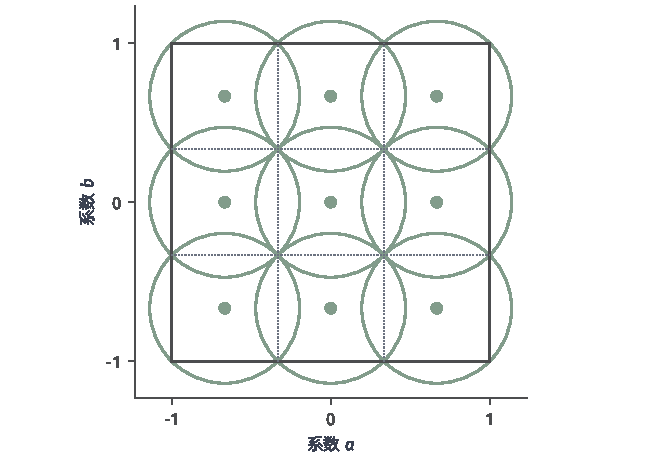
\includegraphics[width=112.0mm]{figures/01-mathematical-preliminaries-upper/02-linear-algebra-and-geometry/matplotlib/concepts-analysis-functional/covering-centers.pdf}
 \functionalinlinefigurecaption{fig:functional-covering-centers}
   {仿射函数族的有限覆盖。方形表示$a,b\in[-1,1]$，九个实心点是类内代表，圆的半径为$\sqrt2/3$。每个小方格都被对应格心的闭球覆盖；圆的重叠与越出方形的部分均不影响覆盖要求。}
\end{minipage}
\end{center}

覆盖结构还可以由函数类运算传播。若$\mathcal{F}$与$\mathcal{G}$在同一上确界距离下
分别有$\varepsilon_F$与$\varepsilon_G$覆盖，则
\[
  \mathcal{F}+\mathcal{G}
  =
  \{f+g:f\in\mathcal{F},\ g\in\mathcal{G}\}
\]
有半径$\varepsilon_F+\varepsilon_G$、大小至多为两个覆盖大小乘积的覆盖。若
$\varphi:\mathbb{R}\to\mathbb{R}$是$L$-Lipschitz函数，则把
$\mathcal{F}$的$\varepsilon$-覆盖逐点送入$\varphi$，得到
$\varphi\circ\mathcal{F}$的$L\varepsilon$-覆盖。
前一项由
$\lVert(f+g)-(\widetilde f+\widetilde g)\rVert_\infty
\leq\lVert f-\widetilde f\rVert_\infty+\lVert g-\widetilde g\rVert_\infty$
保证，后一项由
$\lVert\varphi\circ f-\varphi\circ\widetilde f\rVert_\infty
\leq L\lVert f-\widetilde f\rVert_\infty$保证；构造出的中心仍属于相应的新函数类。
当$L=0$时，复合类只含同一个常函数，一个中心就是零半径覆盖。
这些关系说明组合结构怎样累积
复杂度，却不自动给出有限样本泛化结论。

覆盖数随距离与误差半径改变，组合维度则随输出区分规则改变。二者都需要明确函数类
与输入对象；把计数界或覆盖界用于学习保证时，还要另加抽样和概率条件。


固定输入距离把$x_1,\ldots,x_n$预先固定。序贯问题允许第$t$个输入根据此前反馈变化，
单个输入序列因而不能列出所有可能路径。这里用二叉树表达分支，并以
$\epsilon_t\in\{-1,1\}$标记第$t$步选择的分支；$\epsilon_t$只是抽象路径标签，不必
等于实值函数输出$f(\bm{x}_t)$。若具体问题的反馈不是二元值，还需另行给出编码规则或
改用相应的分支集合。
\begin{definition}[二叉查询树]
\label{def:functional-query-tree}
设$\mathcal X$为非空输入集合，$T\geq1$为整数。深度为$T$的\term{查询树}（query tree）由映射
\[
  \bm{x}_t:\{-1,1\}^{t-1}\to\mathcal{X},
  \qquad t=1,\ldots,T,
\]
组成。这里$\{-1,1\}^0$只有空路径，根节点因而是一个固定输入$\bm{x}_1$；在路径
$\bm{\epsilon}=(\epsilon_1,\ldots,\epsilon_T)$上，第$t$步访问
$\bm{x}_t(\epsilon_1,\ldots,\epsilon_{t-1})$。同一个函数$f$沿该路径产生
\[
  \bigl(
    f(\bm{x}_1),
    f(\bm{x}_2(\epsilon_1)),
    \ldots,
    f(\bm{x}_T(\epsilon_1,\ldots,\epsilon_{T-1}))
  \bigr).
\]
\end{definition}
树同时编码所有按过去分支的输入选择规则，本身没有给路径指定概率。

图~\ref{fig:functional-query-tree}只展开两层，便能看见这一信息约束：查询$x_0$之后，
下一次查询取$x_-$还是$x_+$由已出现的分支决定。覆盖中心必须提前为两个可能的下一步
都指定值，不能在分支确定后临时增加一棵新的中心树。
\begin{center}
\begin{minipage}{\linewidth}
 \centering
 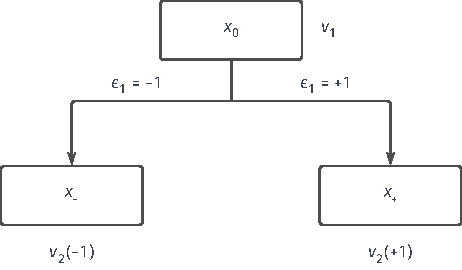
\includegraphics[width=78.281mm]{figures/01-mathematical-preliminaries-upper/02-linear-algebra-and-geometry/tikz/concepts-analysis-functional/query-tree.pdf}
 \functionalinlinefigurecaption{fig:functional-query-tree}
   {深度为$2$的固定查询树。根查询$x_0$，左右分支对应$\epsilon_1=-1$与$+1$；各节点旁的$v_1,v_2(\pm1)$是一棵覆盖中心预先指定的值，表示近似值而非真实反馈。固定一条路径只读取根节点与该分支的下一步输入，整棵树还保留另一种可能。}
\end{minipage}
\end{center}

在固定输入上，覆盖中心是一组函数值；在查询树上，它必须为每个可能访问的节点预先
指定一个实数。下面的覆盖条件沿每条路径比较误差，中心集合仍在路径出现之前确定。
\begin{definition}[序贯覆盖与序贯覆盖数]
\label{def:functional-sequential-cover}
给定深度为$T$的查询树$\bm x$、非空实值函数类$\mathcal F$和$\varepsilon>0$。
实数树$v=(v_t)$的每层映射为$v_t:\{-1,1\}^{t-1}\to\mathbb R$。若这些树组成的
有限集合$\mathcal C$满足：对每个$f\in\mathcal F$和每条路径$\bm\epsilon\in\{-1,1\}^T$，
都存在$v\in\mathcal C$使
\begin{equation}
  \left(
    \frac1T\sum_{t=1}^{T}
    \left|
      f\bigl(\bm{x}_t(\epsilon_{1:t-1})\bigr)
      -
      v_t(\epsilon_{1:t-1})
    \right|^2
  \right)^{1/2}
  \leq\varepsilon,
  \label{eq:functional-sequential-cover}
\end{equation}
则称$\mathcal C$为该查询树上的序贯$\varepsilon$-覆盖。其最小大小记为
$N_2^{\mathrm{seq}}(\varepsilon,\mathcal F,\bm x)$；不存在有限覆盖时取$+\infty$。
再定义
\[
 N_2^{\mathrm{seq}}(\varepsilon,\mathcal F,T)
 =\sup_{\bm x:\,\text{深度为 }T}
 N_2^{\mathrm{seq}}(\varepsilon,\mathcal F,\bm x),
\]
其中上确界遍历全部深度为$T$的查询树。这一最坏树量衡量同一函数类在该深度下
应对所有允许查询规则所需的覆盖规模。
\end{definition}
覆盖集合必须在选择具体函数与路径之前固定，
其中每个$v$都为整棵树的节点赋值，并且第$t$层的值只依赖此前分支
$\epsilon_{1:t-1}$。针对不同的$f$与路径可以从该固定集合中选择不同$v$；不能做的是在
看到完整未来后临时构造一个不属于预定覆盖集合的数值序列。正是这种树形、非前视的中心
保留了序贯信息约束。

序贯覆盖数对所有深度$T$查询树取最坏情形。比较固定输入与查询树之前，必须统一覆盖
中心的约定：上一小节要求中心属于$\mathcal F$，这里的实数树却不必由某个
$f\in\mathcal F$产生。因此在同一半径下，不能直接断言序贯覆盖数更大。例如
$T=1$、$\mathcal F=\{f_-,f_+\}$，其中$f_-\equiv-1$、$f_+\equiv1$，取
$\varepsilon=1$。内部中心的固定覆盖需要两个函数，外部中心$v_1=0$却能同时覆盖二者。

若固定输入的中心也允许是任意实值取值向量，则不分支查询树与这一外部中心覆盖一致，
对所有查询树取最坏情形才保证不小于对所有固定输入取最坏情形。对固定输入上的外部覆盖，若保留内部中心约定，
可在每个被函数类占据的外部$\varepsilon$球中选一个类内代表；三角不等式给出内部
$2\varepsilon$覆盖，数量不增加。这个两倍半径的换算不能省去。反向比较仍需额外规则性。
上述换算只对固定输入的取值向量逐球选代表；一般中心树可能在不同路径上分别
接近不同函数，不一定有同一个函数能在所有路径上接近它，因此不能把这个换算
不加证明地推广到任意外部中心树。
与胖打散维相似，还可以定义带间隔的序贯打散维；它衡量函数类能否沿树的每条分支持续作出可分辨选择。这里仅建立输入可适应变化时使用的结构对象。概率界、在线遗憾和自适应采样保证，
还需分别加入相应的随机或算法条件。

深度为$2$的树已经能展示固定覆盖与序贯覆盖的差别。设根节点查询$x_0$；沿标签
$\epsilon_1=-1$的分支查询$x_-$，沿标签$\epsilon_1=1$的分支查询$x_+$，并假设函数
在这三个点上的值都属于$[-B,B]$。把三个节点值分别量化到宽度不超过$\varepsilon$的
区间，并为
每个被函数类占据的三维网格单元保留一棵代表函数树，就得到序贯
$\varepsilon$-覆盖：左路径比较$(x_0,x_-)$上的两个值，右路径比较
$(x_0,x_+)$上的两个值，每条路径的均方根误差都不超过$\varepsilon$。固定两点覆盖
只需描述一条已经选定的路径；树覆盖必须在分支发生前同时准备$x_-$与$x_+$处的值。
因此，不能等路径进入某个分支后，再用一个未属于预定覆盖集合的新近似器补上所选分支。
若每个节点最多使用$Q=1+\lceil2B/\varepsilon\rceil$个量化区间，这个构造至多
保留$Q^3$棵中心树；它是一个可检验的上界，不是最小序贯覆盖数的公式。

回到$f_\star(x)=|x-1/2|$，Bernstein多项式在一致范数下随次数增加逼近它；
含结点$1/2$的线性样条与两个ReLU单元则能精确表示它。前者的每个基系数影响全域，
样条的结点值只影响相邻片段，ReLU单元决定折点及一侧的斜率变化。
这些是对同一个目标的表示结论，不是整个函数类共享一个有限覆盖的结论。
核截面与这些表示的差异见表~\ref{tab:functional-representation-comparison}；
概率误差和在线算法保证也不由本节的确定性计数自动产生。

\section{扰动与稳定性}
\label{sec:functional-stability}

预测值、拟合函数与平滑目标并不是同一种输出。
固定函数范数以后，读取和变换的有界性控制输出误差；
拟合解还受目标、观测与惩罚尺度影响，离散能量则受边权与搬运规则影响。
下面按这些输出分别分析扰动，保留各自的比较尺度。

\subsection{运算的误差传播}
\label{sec:functional-operation-stability}

固定有界算子$A$时，$\lVert A(f+h)-Af\rVert\leq\lVert A\rVert_{\mathrm{op}}\lVert h\rVert$。
算子再变为$\widetilde A$时，
\[
 \lVert\widetilde A(f+h)-Af\rVert
 \leq\lVert\widetilde A\rVert_{\mathrm{op}}\lVert h\rVert
       +\lVert\widetilde A-A\rVert_{\mathrm{op}}\lVert f\rVert.
\]
两种扰动分别改变输入函数和作用规则，比较前必须使定义域与输出尺度相容。

RKHS中固定位置的读取界为$\sqrt{K(x,x)}$；位置由$x$变为$z$，
还需$|f(x)-f(z)|\leq\lVert f\rVert\lVert K_x-K_z\rVert$。
连续核保证截面随位置连续，任意正定核却不自动有此性质。
尖峰例子则说明$L^2$误差小不控制点值，求导也可能放大高频误差：
在圆上取$f_n(\theta)=n^{-1}\sin(n\theta)$，
函数$L^2$范数趋零，一阶导数范数保持正值。
若改用同时控制导数的Sobolev范数，输入误差的含义已改变，不能仍称相同的稳定性结论。

\subsection{函数解的稳定性}
\label{sec:functional-solution-stability}

固定读取方向与$\lambda>0$，平方拟合的代表系数满足
$(\bm G+n\lambda\bm I)\bm a=\bm y$。
当目标读数改为$\bm y+\delta\bm y$时，
$\delta\bm a=(\bm G+n\lambda\bm I)^{-1}\delta\bm y$，故
$\lVert\delta\bm a\rVert_2\leq\lVert\delta\bm y\rVert_2/(n\lambda)$。
函数和读数分别满足
\[
 \lVert\delta f\rVert_{\mathcal H}^2
 =\delta\bm y^\top(\bm G+n\lambda\bm I)^{-1}
      \bm G(\bm G+n\lambda\bm I)^{-1}\delta\bm y
 \leq\frac{\lVert\delta\bm y\rVert_2^2}{4n\lambda},
 \qquad
 \lVert\bm G\delta\bm a\rVert_2\leq\lVert\delta\bm y\rVert_2.
\]
第一界使用$t/(t+n\lambda)^2\leq1/(4n\lambda)$，第二界使用$t/(t+n\lambda)\leq1$。
系数、函数与预测的放大率不同，不能用其中一个代替其余输出。

整体误差拟合中的谱收缩$t/(t+\lambda)$同样使$L^2$目标扰动的解响应不超过输入误差；
RKHS尺度则对小$t$方向另外计价。具体地，减小$\lambda$会减小
正谱解相对$y_+$的$L^2$收缩误差；零空间分量$y_0$留下的误差不变。
与此同时，由$t/(t+\lambda)^2\leq1/(4\lambda)$得到的
$L^2$目标扰动到RKHS解扰动的放大上界为$1/(2\sqrt\lambda)$，会随$\lambda$减小而增大。
这描述的是核范数响应的上界，不能据此声称$L^2$解响应超过输入误差。
若核改变，读取方向与候选空间也会改变，必须先选共同的点值或$L^2$输出尺度。
在有限矩阵层面，令$\bm B=\bm G+n\lambda\bm I$，
当$\lVert\bm B^{-1}\bm E\rVert<1$时，第~\ref{chap:linear-algebra-and-matrix-analysis}章的反演扰动界控制$(\bm B+\bm E)^{-1}$；
这只控制相应坐标计算，函数重构还要计入核截面本身的变化。

\subsection{离散目标的稳定性}
\label{sec:functional-discrete-objective-stability}

在已规定的离散标量能量上，固定函数记录$\bm f$，边权变化$\delta w_{i,j}$产生
\[
 |\widetilde{\mathcal E}_n(\bm f)-\mathcal E_n(\bm f)|
 \leq\tfrac12\sum_{i,j}|\delta w_{i,j}|(f_i-f_j)^2.
\]
这个界比较同一个记录在两个二次型中的目标值。位置扰动还可能改变读数、邻域与权重，
硬阈值跨越时边集合会突变，不能只用光滑权重的微小变化解释。
向量场能量另有搬运误差：固定一条边，若差向量由$\bm d$变为$\bm d+\bm e$，
则平方代价变化的绝对值不超过$2\lVert\bm d\rVert\lVert\bm e\rVert+\lVert\bm e\rVert^2$；
再计入度量和边权变化，才得到总目标响应。

采样密度、边界规则或能量中的体积权重变化可能改变所逼近的连续目标，
这需要回查第\ref{sec:functional-sampled-energy-approximation}节的一致性条件。
若只改变优化用的内积，目标函数并未改变，梯度及演化过程会改变；
若该权重同时进入目标二次型，最优任务也已变化。离散非负性不能替代这两种判断。

\section{本章小结}
\label{sec:functional-summary}
\label{sec:functional-analysis-approximation-summary}


函数空间沿用线性组合与几何输入域，却必须重新检查整体误差、极限归属和读取是否良定义。
Hilbert完备性与闭性让最近分量存在，Riesz表示把稳定读取变为方向，
核空间进一步使点值读取可由空间范数控制。积分变换、空间微分与目标微分分别改变函数、
读取局部变化和评价整个函数的扰动。

有限观测、整体误差与平滑能量定义不同的求解任务。
有限表示定理减少不可见方向，不单独保证存在、系数唯一或算法收敛；
展开截断、表示规模、采样与惩罚尺度又分别控制不同的逼近误差。
覆盖数进一步要求：给定精度后，预先准备有限个代表，以同一误差规则近似整个函数类；
这比逐个目标寻找逼近函数增加了统一要求。序贯覆盖的中心还要在未来分支出现前固定为树，
再对允许的查询树取最坏情形，才能保留输入依过去反馈改变的信息限制。
运算、解和离散目标的扰动分析必须固定输出尺度，才能解释可靠性。

\begin{table*}[htbp]
\centering
\begin{tabularx}{\linewidth}{@{}lXXX@{}}
\toprule
研究维度 & 线性空间 & 非线性空间与流形 & 函数空间\\
\midrule
元素与表示 & 全局基与有限坐标 & 局部图与坐标过渡 & 整函数、参数与读数\\
关系与结构 & 包含、位置、距离与等价 & 邻域、切向、距离与轨道 & 成员、整体距离与等价类\\
运算与映射 & 映射组合、分解与矩阵函数 & 微分、搬运、位置更新与体积 & 投影、读取、积分及两种微分\\
方程与优化 & 等式、残差与双侧矩阵方程 & 坐标、轨迹、最短路与点优化 & 最近函数、拟合与平滑能量\\
收敛与逼近 & 对象、幂、迭代与秩预算 & 点、迭代及采样几何 & 函数、截断及表示与采样条件\\
扰动与稳定性 & 运算、解、谱与矩阵函数 & 方向、坐标、拓扑与路径 & 运算、函数解与离散目标\\
\bottomrule
\end{tabularx}
\caption{三类空间在共同研究维度中的对照。有限维赋范空间是完备的，其线性子空间是闭的，以它为定义域且以赋范空间为陪域的
线性映射有界；进入无限维后，这些性质需要分别检验。流形的局部线性方向也不能替代
全局可行位置。}
\label{tab:spaces-six-dimension-comparison}
\end{table*}
